\input{setup}

\pagestyle{fancy}
% \renewcommand{\sectionmark}[1]{\markboth{ #1}{}}
% \renewcommand{\subsectionmark}[1]{\markboth{\thesection\ #1}{\thesubsection\ #1}}
\fancyhf{}
% \rhead{\fontfamily{\sfdefault}\selectfont \textbf{\rightmark}}
% \lhead{\fontfamily{\sfdefault}\selectfont \textbf{Thesis}}
% \rfoot{\fontfamily{\sfdefault}\selectfont \textbf{Page \thepage}}
% \lfoot{\fontfamily{\sfdefault}\selectfont \textbf{Cole Nielsen}} % \today
\fancyhead[LE,RO]{\fontfamily{\sfdefault}\selectfont \textbf{\rightmark}}
% \fancyhead[RE,LO]{Guides and tutorials}
% \fancyfoot[CE,CO]{\rightmark}
\fancyfoot[LE,RO]{\fontfamily{\sfdefault}\selectfont \textbf{Page \thepage}}
\title{\textbf{}}
\date{}

\sloppy\RaggedRight\raggedbottom
\begin{document}	
		% \maketitle 
	% \renewcommand{\familydefault}{\sfdefault}
	\thispagestyle{firstpage}
	\fontfamily{\sfdefault}\selectfont 
	\includegraphics[width=0.5\linewidth]{logo_ntnu_eng_black.png} \\
	\vspace{8em}
	\huge Ultra Low Power Frequency Synthesizer\\	
	\vspace{3em}
	\huge \textbf{Cole Nielsen}\\
	\vspace{12em}
	\large%
	%Electronic Systems Design, Master's Thesis\\
	Master's thesis in Electronic Systems Design\\
	\vspace{4pt}
	\FloatBarrier

	\def\arraystretch{1.3}
	\setlength{\tabcolsep}{1em}
	\begin{tabular}{@{} l  l}
	Submission date: & June 2020\\
	Supervisor: & Trond Ytterdal, IET\\
	Co-supervisor: & Carsten Wulff, IET\\
	\end{tabular} \\
	\FloatBarrier
	\vspace{3em}
	Norwegian University of Science and Technology \\ 
	\vspace{4pt}Department of Electronic Systems\\
	
	% \begin{center}
	% 	\large
	% 	\begin{tabular}{ l r }
	% 		\textbf{Name} & Cole Nielsen \\
	% 		\textbf{Assigned N$^\textbf{\textnormal{o}}$} & 13 \\
	% 		\textbf{Term} & Autumn 2018\\
	% 		\textbf{Instructor} & Guennadi Kouzaev\\
	% 	\end{tabular}
	% \end{center}
	% \vspace{2em}
	% \vhrulefill{\lineheight}
	\pagebreak
	\thispagestyle{blank}
	\null\pagebreak

	% % % % % % % % % % % % % % % % % % % % % % % % % % % % % % % % % % % % 
	% Abstract
	\justify
	\setcounter{page}{1}
	% \pagebreak
	\thispagestyle{nohdr}
	\large\fontfamily{\sfdefault}\selectfont \		
	\begin{abstract} \large\fontfamily{\rmdefault}\selectfont \
		
		\vspace{-2em}An integer-N all digital phase locked loop (ADPLL) frequency synthesizer implemented 22nm FD-SOI (22FDX) technology is presented in this paper, achieving a power consumption of \hl{X} $\mu$W at 2.448 GHz, a jitter FOM of \hl{X} dB, and an active area of \hl{X} mm$^2$. This design emphasizes power reducing architectural choices for application to low duty cyce wake up receivers (WURx), utiling low complexity, bias and reference free circuits. Included is a novel, pseudo-differential voltage controlled ring oscillator utilizing FD-SOI backgates to implement both frequency tuning and differential behavior. This oscillator achieves high oscillator tuning gain with rail-to-rail input range, whilst utilizing no current biasing. Capactive DACs are utilized to provide digital control to the oscillator with minimum power draw. A low complexity band-bang phase detector (BBPD) and all digital loop filter, with no divider in steady state implement the remaining portions of the PLL. Calibration of the PLL is implemented utilizing a synchronous counter-based frequency error detection scheme coupled with a coarse bank of tuning capacitors.
	\end{abstract}
	% \section*{Abstract}
	% fjdsfkajjlkf

	% % % % % % % % % % % % % % % % % % % % % % % % % % % % % % % % % % % % 
	% Preface
	\pagebreak
	\thispagestyle{nohdr}
	\null\pagebreak
	\thispagestyle{nohdr}
	\large\fontfamily{\sfdefault}\selectfont 
	\Huge\textbf{Preface.}\\
	\epigraph{Simplicity is the ultimate sophistication.}{\textit{Leonardo da Vinci}}
	\large\fontfamily{\rmdefault}\selectfont 
	\vspace{1em}
	I would like to thank my advisors Trond Ytterdal and Carsten Wulff for providing me the oppourtunities to futher my knowledge and experience in the dark arts of circuit design.

	\par I also thank my family for their continual open support of my life endeavors.


	% % % % % % % % % % % % % % % % % % % % % % % % % % % % % % % % % % % % 


	% % % % % % % % % % % % % % % % % % % % % % % % % % % % % % % % % % % % 
	% Project Description
	\pagebreak
	\thispagestyle{nohdr}
	\null\pagebreak
	\thispagestyle{nohdr}
	\large\fontfamily{\sfdefault}\selectfont 
	\Huge\textbf{Problem description.}\\
	% \vspace{1em}
	\large\fontfamily{\rmdefault}\selectfont 
	
	The intent of this project is to develop an ultra low power, integer-N ADPLL frequency synthesizer for applications to wake up receiver (WURX) radio circuits. The target technology is Global Foundaries 22FDX fully-depeleted silicon on insulator (FD-SOI), a 22nm process node. The implemented PLL is intended for use in duty cycled wake up receiver WURX circuits applications, with on the order of 1\% active time. Thus, the design must feature low power consumption in inactive (sleep) states, and rapid wake-up/resume. The required specifications for this PLL design are given in table \ref{reqs}\\
		\begin{table}[htb!]
			\centering
			\def\arraystretch{1.5}		
			\setlength\arrayrulewidth{1pt}
			\setlength{\tabcolsep}{1em} % for the horizontal padding
			\fontfamily{\sfdefault}\selectfont 
			\begin{tabular}{|l|r|l|}	
				\hline 
				\rule[-1ex]{0pt}{2.5ex} \cellcolor{gray!40}\textbf{Parameter} & \cellcolor{gray!40}\textbf{Specification} & \cellcolor{gray!40}\textbf{Unit}\\ 
				\hline 
				\rule[-1ex]{0pt}{2.5ex} Power & $\leq$ 100 &  $\mu$W  \\ 
				\hline 
				\rule[-1ex]{0pt}{2.5ex} CNR\tablefootnote{Carrier to noise ratio.} & $\geq$ 20 &  20 dBc  \\ 
				\hline 
				\rule[-1ex]{0pt}{2.5ex} Reference frequency\tablefootnote{Divided frequencies (powers of 2) are also acceptable.} &  32  &  MHz  \\ 
				\hline 
				\rule[-1ex]{0pt}{2.5ex} Synthesized frequency & 2.448 &  MHz  \\ 
				\hline 
				\rule[-1ex]{0pt}{2.5ex} Area & $\leq$ 0.01 &  mm$^2$  \\ 
				\hline 
				\rule[-1ex]{0pt}{2.5ex} Lock time (cold-start) & $\leq$ 20 & $\mu$s  \\ 
				\hline 
				\rule[-1ex]{0pt}{2.5ex} Re-lock time (sleep-resume) & $\leq$ 5 & $\mu$s  \\ 
				\hline 
				\rule[-1ex]{0pt}{2.5ex} FOM$_{\Phi n}$\tablefootnote{ FOM$_{\Phi n} = 10\log_{10}\left(\frac{\sigma_{t_j}^2}{(\textnormal{1 s})^2}\cdot\frac{\textnormal{Power}}{\textnormal{1 mW}}\right)$, where $\sigma_{t_j}$ is the measured RMS timing jitter of the PLL.} & $\leq$ -230 & dB  \\ 
				\hline 
			\end{tabular} 
			\caption{Design required specifications.}
			\label{reqs}
		\end{table} 
	\large\fontfamily{\rmdefault}\selectfont 
	\par This work is in part a continuation of the author's previous work \cite{Me} on the optimization and simulation of integer-N ADPLL, which focused on automation of loop filter design. The architectural proceeded with in this work are motivated through findings of this work, particularly the usage of bang-bang phase detector with proportional-integral (PI) controller based loop filter. This architecture was found to be advantageous in terms of complexity and optimizability, providing for a known good starting point on this project.

	% % % % % % % % % % % % % % % % % % % % % % % % % % % % % % % % % % % % 
	% % Preface
	% \pagebreak
	% \thispagestyle{nohdr}
	% \null\pagebreak
	% \thispagestyle{nohdr}
	% \large\fontfamily{\sfdefault}\selectfont 
	% \Huge\textbf{Preface.}\\
	% \vspace{1em}
	% \large\fontfamily{\rmdefault}\selectfont 
	% \lipsum[1]

	% % % % % % % % % % % % % % % % % % % % % % % % % % % % % % % % % % % % 
	% Contents, list of tables and figures
	\fontfamily{\sfdefault}\selectfont 
	\thispagestyle{nohdr}
	\null\pagebreak
	\thispagestyle{nohdr}
	\null\pagebreak
	\tableofcontents
	\pagebreak
	\listoffigures
	\listoftables

	% \vhrulefill{\lineheight}

	\fontfamily{\rmdefault}\selectfont 
	% % % % % % % % % % % % % % % % % % % % % % % % % % % % % % % % % % % % 
	% Abbreviations
	\pagebreak
	\FloatBarrier
	\section*{Abbreviations.}
	\begin{table}[htb!]
	\renewcommand*{\arraystretch}{1.30}\large
	\begin{tabular}{@{}ll}
		\textbf{\textsf{ADPLL}}	&	All digital phase locked loop \\
		\textbf{\textsf{BBPD}}	&	Bang-bang phase detector \\
		\textbf{\textsf{BOX}}	&	Burried-oxide \\
		\textbf{\textsf{BW}}	&	Bandwidth \\
		\textbf{\textsf{CDAC}}	&	Capacitive digital to analog converter \\
		\textbf{\textsf{CDF}}	&	Cumulative distribution function \\
		\textbf{\textsf{CI}}	&	Confidence interval \\
		\textbf{\textsf{CLK}}	&	Clock \\
		\textbf{\textsf{CM}}	&	Common mode \\
		\textbf{\textsf{CMOS}}	&	Complementary metal oxide semiconductor \\
		\textbf{\textsf{CMRR}}	&	Common mode rejection ratio \\
		\textbf{\textsf{CNR}}	&	Carrier to noise ratio \\
		\textbf{\textsf{DAC}}	&	Digital to analog converter \\
		\textbf{\textsf{DC}}	&	Direct current \\
		\textbf{\textsf{DCO}}	&	Digitally controlled oscillator \\
		\textbf{\textsf{DFF}}	&	D flip flop \\
		\textbf{\textsf{DIV}}	&	Divider \\
		\textbf{\textsf{DNL}}	&	Differential non-linearity \\
		\textbf{\textsf{FDSOI}}	&	Fully depleted silicon on insulator \\
		\textbf{\textsf{FET}}	&	Field effect transistor \\
		\textbf{\textsf{FOM}}	&	Figure of merit \\
		\textbf{\textsf{FSK}}	&	Frequency shift keying \\
		\textbf{\textsf{FSM}}	&	Finite state machine \\
		\textbf{\textsf{HVTPFET}}	&	High threshold voltage PFET \\
		\textbf{\textsf{IIR}}	&	Infinite impulse response \\
		\textbf{\textsf{INL}}	&	Integral nonlinearity \\
		\textbf{\textsf{ISF}}	&	Impulse sensitivity function \\
		\textbf{\textsf{KDCO}}	&	DCO Gain \\
		\textbf{\textsf{LC}}	&	Inductor-capacitor \\
		\textbf{\textsf{LF}}	&	Loop filter \\
		\textbf{\textsf{LO}}	&	Local oscillator \\
		\textbf{\textsf{LSB}}	&	Least significant bit \\
		\textbf{\textsf{LVTNFET}}	&	Low voltage threshold NFET \\
		\textbf{\textsf{MMSE}}	&	Minimum mean squared error \\
		\textbf{\textsf{MOSFET}}	&	Metal oxide semiconductor filed effect transistor \\
	\end{tabular}
	\end{table}
	\begin{table}[htb!]
	\renewcommand*{\arraystretch}{1.30}\large
	\begin{tabular}{@{}ll}
		\textbf{\textsf{MSE}}	&	Mean squared error \\
		\textbf{\textsf{NFET}}	&	N-channel field effect transistor \\
		\textbf{\textsf{NMOS}}	&	N-channel metal oxide semiconductor \\
		\textbf{\textsf{OOK}}	&	On-off keying \\
		\textbf{\textsf{OTW}}	&	Oscillator tuning word \\
		\textbf{\textsf{PD}}	&	Phase detector \\
		\textbf{\textsf{PDF}}	&	Probability distribution function \\
		\textbf{\textsf{PFET}}	&	P-channel FET \\
		\textbf{\textsf{PI}}	&	Proportional-integral \\
		\textbf{\textsf{PID}}	&	Proportional-integral-derivative \\
		\textbf{\textsf{PLL}}	&	Phase locked loop \\
		\textbf{\textsf{PMOS}}	&	P-channel metal oxide semiconductor \\
		\textbf{\textsf{PN}}	&	Phase noise \\
		\textbf{\textsf{PSD}}	&	Power spectral density \\
		\textbf{\textsf{PSK}}	&	Phase shift keying \\
		\textbf{\textsf{PVT}}	&	Process \\
		\textbf{\textsf{RC}}	&	Resistor-capacitor \\
		\textbf{\textsf{RMS}}	&	Root mean squared \\
		\textbf{\textsf{RO}}	&	Ring oscillator \\
		\textbf{\textsf{RST}}	&	Reset \\
		\textbf{\textsf{RVT}}	&	Regular voltage threshold \\
		\textbf{\textsf{SLVTNFET}}	&	Super-low voltage threshold NFET \\
		\textbf{\textsf{SNR}}	&	Signal to noise ratio \\
		\textbf{\textsf{SOI}}	&	Silicon on insulator \\
		\textbf{\textsf{SSB}}	&	Single side band \\
		\textbf{\textsf{TDC}}	&	Time to digital converter \\
		\textbf{\textsf{TF}}	&	Transfer function \\
		\textbf{\textsf{TSPC}}	&	True single phase circuit \\
		\textbf{\textsf{UTBB}}	&	Ultra-thin body BOX \\
		\textbf{\textsf{VCO}}	&	Voltage controlled oscillator \\
		\textbf{\textsf{WUC}}	&	Wake up call \\
		\textbf{\textsf{WUR}}	&	Wake up receiver \\
	\end{tabular}
	\end{table}

	\FloatBarrier\pagebreak
	\null

	% % % % % % % % % % % % % % % % % % % % % % % % % % % % % % % % % % % % 
	\pagebreak\FloatBarrier

	\section{Introduction}\label{intro}
	Phase locked loops (PLLs) are the fundamental building block to virtually all wired and wireless communication systems of today. To meet industrial demands of continual and uncompromising improvement of communication system performance, i.e. higher data rates, lower power, it is paramount that PLL performance is continually improved. Of perpetually growing importance is the application of PLLs to radios in battery powered mobile and IoT devices, for which reduction of power is highly sought after. A recent approach to reducing power consumption in such wireless applications is through usage of wake up receivers (WUR). These are ultra low power, low data rate radio receivers, which listen for requests (i.e. a "wake up call", or WUC) for activity from some external source. Upon a WUC, the device powers on and activates a higher powered radio supporting higher data rates for only the time required. In devices which are inactive for substantial periods of time, waiting for requests for activity (e.g. as with sensor networks or wireless headphones), such a scheme can enable great power reduction, for example achieving 4.5 nW in \cite{Jiang2017} and 365 nW in \cite{Sadagopan2017} for 2.4 GHz band WUC reception. When this is compared to utilizing a full data rate receiver to poll the radio spectrum for activity requests, which for a state of art Bluetooth design may draw on the order of 1.9 mW \cite{Tamura2020}, it is seen that upwards of $10^6$ improvement in power is obtainable, undoubtedly reducing power consumption.

Thus, in this work, the design of a low power PLL which enables WUR applications is considered. Ultra low power consumption has been achieved with PLL-less on-off keying receivers, for example achieving 4.5 nW with 0.3 kbps of data at 2.4 GHz \cite{Jiang2017}. However, this work will be catered to PLL-based designs that maintain backwards-compatibility with FSK and PSK modulation schemes supported by existing wireless standards such as 802.15.4, WiFi and Bluetooth. A review of current literature shows that state of art within ultra low power PLLs in the 2.4GHz band regime achieve power consumption on the order of hundreds of $\mu$W, for example 170 $\mu$W in \cite{Zhang2019}, 265 $\mu$W in \cite{Liu2019}. Therefore, to advance the boundary of current state of art, this work seeks to achieve a new record for PLL power consumption, namely $\leq$ 100 $\mu$W for use in 2.4 GHz band radio operation. Furthermore, an attempt will be made to minimize implemented area of the PLL. Current state of art for PLL area rests in the sub-0.01 mm$^2$ regime, with as small as 0.0036 mm$^2$ being achieved in 5nm process technology \cite{Liu2020}. It will be attempted to obtain a similar area to the current state of art.
% To meet these goals, a PLL design methodology is described in this work, favoring minimization of overall complexity,educing current braches and circuit area, whilst yielding high performance on a given power budget.


 A brief outline of the paper is as follows. An introduction to PLL and FD-SOI theory is in section \ref{theory}. The undertaken PLL Design is discussed in sections \ref{pll_arch}-\ref{behav_sim}. Simulation results of the implemented design are in section \ref{results}. Comparison to the state of art and general discussion regarding this work is in section \ref{disco}. Finally, section \ref{conclusion} concludes. 
%
%
% Phase locked loops are extraordinarily useful frequency synthesizers that are vital to the operation of virtually all wThe trend towards increasingly lower power wireless devices poses an acute need to reduce PLL power consumption. This is a challenge as PLLs typically rank among the highest power consuming components of a radio, and are necessarily so to limit oscillator phase noise. A sampling of literature on ultra-low power 2.4GHz radios finds oscillator power consumption as a portion of total radio consumption to be 53\% for the receiver in \cite{regulagadda_2018}, 88\% of the transmitter in \cite{shi_2019}, 52\% of the transmitter in \cite{chen_2019}, and 50\% of the receiver in \cite{pengg_2013}. Reducing analog PLL power consumption can be a prohibitive challenge as the performance of analog loop filters degrade as a result of unavoidably lower charge pump current. However, recent CMOS process nodes with minimum gate lengths as small as 7nm allow for all-digital loop filters and PLLs to be a possible alternative to analog designs due to increasingly low power consumption associated with their implementation. Digital loop-filters have the unique advantage where they can be scaled indefinitely as process nodes advance, suffering no loss in performance, while also having greatly reduced sensitivities to process, voltage, temperature (PVT) variations compared to analog implementations.
%
%
% Thus, in this paper, a new framework, \texttt{pllsim}, written in Python\footnote{Python Software Foundation \url{https://www.python.org/}.} is introduced (this framework is available on GitHub\footnote{\texttt{pllsim} codebase: \url{https://github.com/nielscol/pllsim}.}), which uniquely addresses issues of ultra-low power ADPLL design. Specifically, design of integer-N type PLLs is focused on, as the impetus of this work is an integer-N PLL design project. Topics presented are (a) automatic design and optimization of ADPLL loop filters given target system and component level specifications for the PLL, and (b) behavioral time domain PLL simulation for accurate analysis and verification of loop filter and PLL performance, with an integrated Monte-Carlo sampling variation analysis engine. Due to high phase noise associated with low power design, the optimization approach introduced in this paper focuses on the minimization of total integrated phase noise power to allow for maximum PLL performance on a given power budget.
%

\vspace{1em}

\subsection{Main Contributions}
% \vspace{-0.8em}
\begin{enumerate}[itemsep=0pt,label=\protect\mycirc{\arabic*}]
	\setlength\itemsep{-0.8em}
	\item Implementation of a sub-100 $\mu$W ultra-low power, 0.00365 mm$^2$ area CMOS PLL in a 22nm FD-SOI process technology, with state of art FOM$_{jitter}$ within its power regime, and comparable area to current state of art.
	\item Presentation of a novel pseudodifferential ring oscillator circuit topology and theory of operation, utilizing FD-SOI backgates to implement both frequency tuning and differential coupling.
	\item Realization of linear gain voltage controlled oscillator with rail to rail input range. 
	\item Loop filter optimization theory for proportional-integral controller bang-bang phase detector PLLs with noisy phase detectors.
	\item Theoretical figure for FOM$_{jitter}$ performance limit of proportional-integral controller bang-bang phase detector PLLs.
	\item DAC resolution and oscillator frequency gain optimization theory.
	\item A novel pseudodifferential buffer presenting common mode rejection characteristics.
	\item Implementation of low power CDACs.
	\item Implementation of a low power bang-bang phase detector.
	\item Implementation of a low power digital loop filter.
	\item Demonstration of bias current and reference free PLL design.
\end{enumerate}

	\pagebreak\FloatBarrier

	\section{Theory}\label{theory}
		\subsection{Fully Depleted Silicon on Insulator (FD-SOI)}
	FD-SOI is a process technology that implements complementary metal oxide semiconductor (CMOS) transistors with an insulating layer of oxide, referred to as a burried oxide (BOX), between the channel of the transistors and the silicon substrate \cite{Planes2012}. The addition of such an oxide reduces capacitances of the fabricated transistors to the silicon substrate, resulting in lower overall capacitance than in bulk CMOS technologies. Thus higher frequency of operating is possible versus similar sized bulk process nodes. A further feature introduced by FD-SOI technology is the ability to form isolated wells beneath fabricated devices \cite{Wiatr2019}, which remain electrically isolated from the transistors via the BOX and from the substrate due to PN junctions inherent in well formation. This opens the possibility to achieve biasing across a wide voltage range of the regions below individual transistors (both for PMOS and NMOS devices), which enables tuning of individual transistor threshold voltages by exploitation of the MOS body effect. The well beneath a FD-SOI transistor is referred to as the "backgate". The implementation these features in the Global Foundaries 22FDX process is shown in figure \ref{fig:22fdx_wells}. 
	
			\begin{figure}[htb!]
			        \centering
			        \includegraphics[width=1\textwidth, angle=0]{./figs/theory/wiatr1-p4-wiatr-large}
			    \caption{22FDX cross-sectional construction of active devices \cite{Wiatr2019}.}
			    \label{fig:22fdx_wells}
			\end{figure}
	
	\subsection{MOSFET Models}

	\subsubsection{I-V relations}\label{sec:mos_iv}
	Basic models that describe the large signal current-voltage relations of a Metal Oxide Semiconductor Field Effect Transistor (MOSFET) are introduced here, based wholy from \cite{razavi_2017}. For the purposes of this work, a MOSFET is schematically represented in the manner of figure \ref{fig:mos_symbols}, with gate (G), drain (D), source (S) and backgate (B) terminals. Several operating regimes occur depending on the relation of the terminal voltages. Relevant to the scope of this work, are the linear, saturated and velocity saturated regions of MOSFET operation. Nominally, it is expected that when configured as in figure \ref{fig:vgs_sweep}, sweeping the gate-source voltage ($V_{GS}$), with the drain-source voltage ($V_{DS}$) set greater than 0 in the case of a NFET, that an increasing amount of current will enter the MOSFET drain after crossing a threshold voltage ($V_{TH}$). $V_{TH}$ is predominantly dependent of physical configuration of a FET (dimensions, doping, material), however is impacted by the backgate bias in what is termed "the body effect". A more detailed description of each operating regime will be given in the following discourse.

			\begin{figure}[htb!]
			        \centering
			        \includegraphics[width=0.5\textwidth, angle=0]{./figs/theory/fet_symbols}
			    \caption{MOSFET symbols.}
			    \label{fig:mos_symbols}
			\end{figure}

			\begin{figure}[htb!]
			        \centering
			        \includegraphics[width=0.8\textwidth, angle=0]{./figs/theory/vgs_sweep}
			    \caption{Drain current versus gate-source bias.}
			    \label{fig:vgs_sweep}
			\end{figure}


	% \textbf{Subthreshold Region}
	% $\xi$ is a factor of ideality, $V_T = k_B T/q$, where $k_B$ is the Boltzmann constant, T is the temperature in Kelvin, and $q$ represents the elementary charge.
	% \begin{equation}
	% 	I_D = I_0e^{\frac{V_{GS}}{\xi V_T}}
	% \end{equation}

	\textbf{Linear Region}
	Linear MOSFET operation occurs under the circumstances where  $|V_{GS}-V_{TH}| > |V_{DS}|$. The following equation is the I-V relation in this regime, where $\mu_n$ represents the electron mobility of the semiconductor in use (within the FET channel), $C_{ox}$ represents the MOS oxide capacitance. 
	\begin{equation}
		I_D = \mu_x C_{ox} \left(\frac{W}{L}\right)\left[(V_{GS}-V_{TH})V_{DS}-\frac{1}{2}V_{DS}^2\right]
	\end{equation}

	\textbf{Saturation Region}
	Saturation region occurs when $|V_{DS}| > |V_{GS}-V_{TH}|$. Notably, dependence of drain current on $V_{DS}$ is reduced, and in the case of the ideal models considered here, the effect of $V_{DS}$ are completely negated.
	\begin{equation}
		I_D = \frac{1}{2}\mu_n C_{ox} \left(\frac{W}{L}\right)(V_{GS}-V_{TH})^2
	\end{equation}


	\textbf{Velocity-saturation Region}
	In the scenario of high applied fields which arise in a short MOSFET channels, carrier velocity can saturate to a limited velocity, $v_{sat}$. The point at which this effect takes place is device dependent. For approximate consideration it can be understood to occur when $|V_{DS}/L > E_{crit}|$, where $E_{crit}$ is the electric field which the carrier velocity-electric field relation ($v = \mu E$) of the channel semiconductor becomes sub-linear. Below is the MOSFET model under such circumstances.
	\begin{equation}
		I_D = WC_{ox}(V_{GS}-V_{TH})v_{sat}
	\end{equation}

	\subsubsection{Body Effect}
	Application of a bias to the substrate below a bulk MOSFET, or to the well below a FD-SOI MOSFET, has a direct effect on the threshold voltage of a MOSFET. For a bulk MOSFET, change of body bias affects the width of source-drain and source-body depletions, which consequently can increase or decrease the magnitude of the channel depletion charge as seen by the gate terminal needed to achieve channel inversion. This corresponds to a differential in the threshold voltage. The below equation \cite{razavi_2017} quantifies this effect for bulk devices. $\gamma$ is the body effect coefficient, $2\Phi_F$ represents the MOS surface potential. $V_{TH}$ is non-linearly related to the source-body voltage $V_{SB}$.
	\begin{equation}
		V_{TH} = V_{TH0} + \gamma\left( \sqrt{2\Phi_F + V_{SB}} - \sqrt{|2\Phi_F|} \right)
	\end{equation}
	In the case of FD-SOI transistors, the nature of the body effect is modified due to the presence of the BOX. Thus, an approximate derivation for body effect will be provided here. In FD-SOI, the active channel region is thin, and under strong inversion, the entire channel region is depleted of charge. Supposing a channel height Z and channel doping $N_A$, the total charge to deplete the channel for inversion to occur is $Q_{d} = N_AZ$. With oxide capacitance $C_{ox,fg}$ associated with the front gate, the portion of the threshold voltage associated with total depletion of the channel is, from the front gate perspective:
	\begin{equation}
		V_{d,fg} = \frac{Q_d}{C_{ox,fg}} = \frac{N_AZ}{C_{ox,fg}} 
	\end{equation}
	Supposing that the back gate has capacitance of $C_{ox,bg}$, with bias applied $V_{BS}$, the back gate can be seen to "rob" the front gate of $Q_{bg} = C_{ox,bg}V_{BS}$ when in inversion. Thus results in a partial change of the front gate referred voltage required to obtain channel depletion:
	\begin{equation}
		V_{d,fg}^{'} = \frac{Q_d-Q_{bg}}{C_{ox,fg}} = \frac{Q_d}{C_{ox,fg}} - \frac{C_{ox,bg}}{C_{ox,fg}}V_{BS} = V_{d,fg}-\Delta V_{th,bg}
	\end{equation}
	It is noted that this can be writen as the nominal value of $V_{d,fg}$ minus a differential. This differential is the resulting change in threshold voltage due to back gate bias, $\Delta V_{th,bg}$:
	\begin{equation}
		\Delta V_{th,bg}= \frac{C_{ox,bg}}{C_{ox,fg}}V_{BS} 
	\end{equation}	
	This is linear with applied back gate bias, and that the strength of the coupling is tunable by the ratio of front gate and back gate capacitances. Typically this ratio is $<<1$. If we define the body effect coefficient $\gamma$ as:
	\begin{equation}
		\gamma = \frac{C_{ox,bg}}{C_{ox,fg}}
	\end{equation}
	Given a nominal threshold voltage of $V_{TH0}$, in FD-SOI, the threshold voltage can be represented as:
	\begin{equation}\label{eq:body_effect}
		V_{TH} = V_{TH0} - \gamma V_{BS}
	\end{equation}

	\subsubsection{Linearization of MOSFET models}
	Under conditions where a MOSFET is held at near constant bias levels, with only minor variations around the DC operating level, simpler linearized models of the transistors can be developed. For the different operating regions of the MOSFET, the I-V relations can be generalized in terms of the function $I_D(V_{GS}, V_{DS}, V_{BS})$. Linearization is then obtained by calculating the slope of $I_D$ with respect to the potentials $V_{GS}, V_{DS}, V_{BS}$. The resulting parameters (given as equations \ref{eq:gm} to \ref{eq:fet_out_r}) are the transconductance $g_m$, relating gate drive to drain current, transconductance $g_{mb}$, relating body drive to drain current, and resistance $r_o$, relating drain voltage to drain current. Due to linearization, the current contributions are superimposed to determine total drain current. The linearized circuit which replaces the four terminal MOSFET symbols of figure \ref{fig:mos_symbols} is given by the linearized circuit of figure \ref{fig:ss_model}.

	\begin{align}
		g_m & = \frac{\partial }{\partial V_{GS}}I_D(V_{GS}, V_{DS}, V_{BS}) \label{eq:gm}\\
		g_{mb} & = \frac{\partial }{\partial V_{BS}}I_D(V_{GS}, V_{DS}, V_{BS})\\
		r_o &= \left(\frac{\partial }{\partial V_{DS}}I_D(V_{GS}, V_{DS}, V_{BS})\right)^{-1}\label{eq:fet_out_r}
	\end{align}
		\begin{figure}[htb!]
		        \centering
		        \includegraphics[width=1\textwidth, angle=0]{./figs/theory/lin_oppoint}
		    \caption{Transconductances as slope localized at operating point of I-V curve.}
		    \label{fig:lin_oppoint}
		\end{figure}

		\begin{figure}[htb!]
		        \centering
		        \includegraphics[width=0.4\textwidth, angle=0]{./figs/theory/ss_model}
		    \caption{Linearized (small-signal) MOSFET model.}
		    \label{fig:ss_model}
		\end{figure}
		\FloatBarrier
	A useful relation based on this linearization can be determined, based on the FD-SOI body effect equation \ref{eq:body_effect}, and the I-V relations for the three MOSFET operation regions discussed in section \ref{sec:mos_iv}. Computation of $g_{m}$ and $g_{mb}$ for all three regions with the FD-SOI body effect yields the same result given in equation \ref{eq:gm_gmb_relation}. This is that $g_{mb}$ and $g_{m}$ are related by the body effect coefficient $\gamma$.
	\begin{equation}\label{eq:gm_gmb_relation}
	g_{mb} = \gamma g_{m}
	\end{equation}

		



	\subsection{Basic PLL}
	A phase locked loop (PLL) is a feedback system whose output tracks or maintains a fixed phase relationship to an input signal. PLLs are well suited for frequency synthesis, which is the process of generating derivative frequencies from some reference frequency. Given a reference signal with phase trajectory $\Phi_{ref}$ and output signal with phase $\Phi_{out}$, a PLL can be modeled as in figure \ref{fig:basic_fb} using an elementary feedback system, with feedforward and feedback networks A(s) and B(s). 
	\begin{figure}[htb!]
		\center\include{./figs/basic_feedback}
		\caption{Phase locked loop as elementary feedback system.}
		\label{fig:basic_fb}
	\end{figure}
	\FloatBarrier
	The closed loop phase response for $\Phi_{ref}$ to $\Phi_{out}$ is therefore:
	\begin{equation}
		\frac{\Phi_{out}(s)}{\Phi_{ref}(s)} = \frac{A(s)}{1+A(s)B(s)}
	\end{equation}
	A case of interest is when B(s) = 1/N, where N is a constant, and the loop gain L(s) = A(s)B(s) $>>$ 1. The closed loop response for this case is:
	\begin{equation}\label{mult_by_n}
		\frac{\Phi_{out}(s)}{\Phi_{ref}(s)} \approx \frac{A(s)}{A(s)B(s)} = \frac{1}{B(s)} = N
	\end{equation}
	We see that the phase through the PLL is multiplied by a factor of N. If the input phase signal is sinusoidal with frequency $\omega_{ref}$, and likewise the output with $\omega_{out}$, then $\phi_{ref}(t)=\omega_{ref}t$ and $\phi_{out}(t)=\omega_{out}t$. Accordingly:
	\begin{equation}
		\frac{\Phi_{out}(t)}{\Phi_{ref}(t)} = \frac{\omega_{out}t}{\omega_{ref}t} \approx N \hspace{1em} \rightarrow \hspace{1em} \omega_{out} \approx N\omega_{ref}
	\end{equation}
	Therefore, it is observed that a PLL allows for the generation of a new frequency from a reference frequency signal, which is termed as "frequency synthesis". With a feedback division ratio of 1/N, the PLL multiplies the reference frequency by a factor of N. Hereon, the B(s) portion of a PLL feedback network is referred to as a divider, with associated division raito N.

	\subsection{PLL Synthesizer Architecture}
		A typical architecture for implementing a physically realizable PLL frequency synthesizer \cite{Razavi1996DesignOM} is shown in figure \ref{fig:basic_pll}. This PLL is comprised of four components: (1) a phase detector, herein PD, (2) a loop filter, herein H$_{LF}$(s), (3) a voltage controlled oscillator, herein VCO, and (4) a divider, indicated as "$\div$ N" in figure \ref{fig:basic_pll}. In control systems parlance, the loop filter corresponds to a controller, the VCO an actuator, and the divider as feedback.
		\begin{figure}[htb!]
			\center\fontfamily{\sfdefault}\selectfont
% XCircuit output "basic_pll.tex" for LaTeX input from basic_pll.ps
\def\putbox#1#2#3#4{\makebox[0.00000in][l]{\makebox[#1][l]{}\raisebox{\baselineskip}[0.00000in][0.00000in]{\raisebox{#2}[0.00000in][0.00000in]{\scalebox{#3}{#4}}}}}
\def\rightbox#1{\makebox[0.00000in][r]{#1}}
\def\centbox#1{\makebox[0.00000in]{#1}}
\def\topbox#1{\raisebox{-0.60\baselineskip}[0.00000in][0.00000in]{#1}}
\def\midbox#1{\raisebox{-0.20\baselineskip}[0.00000in][0.00000in]{#1}}
   \scalebox{1}{
   \normalsize
   \parbox{4.66667in}{
   \includegraphics[scale=0.70000]{./figs/basic_pll.pdf}\\
   % translate x=344 y=640 scale 0.38
   \putbox{1.05700in}{1.37900in}{1.20}{PD}%
   \putbox{2.42900in}{0.56700in}{1.20}{$\div$ N}%
   \putbox{0.42000in}{1.52600in}{1.20}{$\Phi_{ref}$}%
   \putbox{3.80100in}{1.52600in}{1.20}{$\Phi_{out}$}%
   \putbox{1.99500in}{1.37900in}{1.20}{H$_{LF}$(s)}%
   \putbox{3.15700in}{1.37900in}{1.20}{VCO}%
   \putbox{1.58200in}{0.70700in}{1.20}{$\Phi_{div}$}%
   \putbox{1.56800in}{1.52600in}{1.20}{$\Phi_e$}%
   \putbox{2.63200in}{1.52600in}{1.20}{V$_{ctrl}$}%
   } % close 'parbox'
   } % close 'scalebox'
   \vspace{-\baselineskip} % this is not necessary, but looks better
\fontfamily{\rmdefault}\selectfont

			\caption{High-level PLL Synthesizer Architecture.}
			\label{fig:basic_pll}
		\end{figure}
		\FloatBarrier
		Further explaination of these components will be hereafter made.

		\subsubsection{Phase Detector}
		A phase detector acts as the summation point of figure \ref{fig:basic_fb}, which measures the phase error $\Phi_e$ between the reference signal and the output of the PLL. The phase error is then used by the controller, which is implemented as the loop filter, to adjust the PLL's state. Such a phase detector may also have intrinsic gain, given by $K_{PD}$.
		\begin{equation}
			\Phi_e(s) = K_{PD}(\Phi_{ref}(s) - \Phi_{div}(s))
		\end{equation}

		\subsubsection{Bang-bang phase detector}\label{bbpd_theory}
		% First reference : \cite{toifl_1998}

		\begin{figure}[htb!]
		    \centering
		    \begin{subfigure}{0.5\textwidth}
		        \centering
		        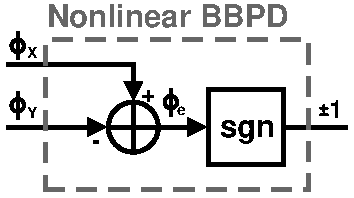
\includegraphics[width=0.75\textwidth, angle=0]{./figs/theory/bbpd_nonlinear}
		        \caption{ }
		        \label{fig:bbpd_nonlinear}
		    \end{subfigure}%
		    \begin{subfigure}{0.5\textwidth}
		        \centering
		        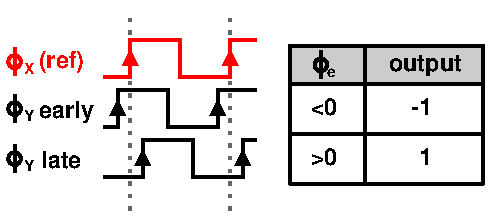
\includegraphics[width=1\textwidth, angle=0]{./figs/theory/bbpd_timing}
		        \caption{ }
		        \label{fig:bbpd_timing}
		    \end{subfigure}
		    % \caption{x.}

		    \caption{\textbf{(a)} BBPD schematic, \textbf{(b)} BBPD timing.}
		    \label{fig:bbpd_theory}
		\end{figure} 
			A simple implementation of a phase detector is a bang-bang phase detector (BBPD) \cite{zanuso_2009}. As exhibited in figure \ref{fig:bbpd_theory}, a BBPD outputs a value of 1 if the input $\Phi_Y$ is late relative to the reference $\Phi_X$ (representing a clock signal), and -1 if it is early. A BBPD shows abrupt nonlinearity in its transfer characteristics. If the error signal variance $\sigma_{\Phi_e}^2$ is constant, which is expected in steady-state PLL operation, a linearized model for phase detector gain can be established \cite{xu_abidi_2017}, given in equation \ref{eq:nom_bbpd_gain}.

			A linearized version of the BBPD is illustrated in figure \ref{fig:bbpd_linearized}. The output $\mathrm{z}$ valued as $\pm 1$ (its variance $\sigma_y^2$=1).
			\begin{equation}\label{eq:nom_bbpd_gain}
				K_{BBPD} = \frac{\mathbb{E}[\Phi_e(t)\cdot\mathrm{z}(t)]}{\mathbb{E}[\Phi_e^2(t)]} = \sqrt{\frac{2}{\pi}}\frac{1}{\sigma_{\Phi_e}}
			\end{equation}
			\begin{figure}[htb!]
				\center\includegraphics[width=0.4\textwidth, angle=0]{./figs/theory/bbpd_linearized}
				\caption{Linearized bang-bang phase detector.}
				\label{fig:bbpd_linearized}
			\end{figure}

			\subsubsection{BBPD Noise}\label{sec:bbpd_noise}
			Given the output of the BBPD is of fixed power $\sigma_z^2$ = 1, a linearized gain of $K_{BBPD}$, a phase error power of $\mathrm{Var}[\Phi_e(t)] = \sigma_{\Phi_e}^2$, and $\mathbb{E}[\Phi_e(t)]=0$, the noise power  $\sigma_{n_{BBPD}}^2$ out of the BBPD is in equation \ref{eq:bbpd_gain}. $K_{BBPD}^2\sigma_{\Phi_e}^2$ represents the power of the phase error signal component post-detector, and it is assumed that noise power and signal power are uncorrelated.
			\begin{equation}\label{eq:bbpd_gain}
				\sigma_{n_{BBPD}}^2 = \sigma_z^2 - K_{BBPD}^2\sigma_{\Phi_e}^2 = 1-\frac{2}{\pi}
			\end{equation}


			Observe that the BBPD noise power is constant. If the reference signal is a clock signal with frequency $f_{ref}$, the BBPD noise spectral density is in equation \ref{eq:bbpd_noise_psd}.
			\begin{equation}\label{eq:bbpd_noise_psd}
				S_{ n_{BBPD}(f)} = \frac{\sigma_{n_{BBPD}}^2}{\Delta f} = \frac{\left(1-\frac{2}{\pi}\right)}{f_{ref}}
			\end{equation}



		\subsubsection{Divider}
			A divider is used as the feedback path in the PLL, where the division ratio N controls the frequency multiplication of a PLL synthesizer. The transfer function of the divider is:
			\begin{equation}
				\mathrm{H}_{div}(s) = \frac{\Phi_{div}(s)}{\Phi_{out}(s)} = \frac{1}{\mathrm{N}}
			\end{equation}


			Dividers are commonly realized as digital modulo-N counters that count oscillation cycles \cite{weste_harris_2011}. With a division ratio of N, the output of the divider will have an active edge transition (considered to be rising edge as shown in figure \ref{fig:digital_div}) every N input cycles. Phase information is inferred from the output edge timing, which occurs with time interval N$/f_{osc}$, and is equal to the point at which output phase equals a multiple of $2\pi$. Thus a digital divider does not provider continuous phase information, but rather a sampled phase signal with rate $f_{osc}/$N. 
			\begin{figure}[htb!]
				\center\include{./figs/digital_div}
				\caption{Digital divider signals.}
				\label{fig:digital_div}
			\end{figure}


		\subsubsection{Loop Filter}
			A loop filter behaves as the controller of a PLL, namely controlling the phase-frequency response of PLL. The choice of loop filter transfer function significatly affects transient PLL behavior, as well as phase noise performance, as is later described. Here, a pole-zero based controller is defined for use in this work. This is designed to have P poles and Z zeros, and can be represented in the canonical form of equation \ref{eq:lf_general_form} as a rational function of polynomials of s with coefficients given with $\{a_0, ..., a_P\}$ and $\{b_0, ..., b_Z\}$.
			\begin{equation} \label{eq:lf_general_form}
				\textnormal{H}_{LF}(s) = \frac{\sum_{j=0}^Z b_js^j}{\sum_{k=0}^P a_ks^k}
			\end{equation}
			
		\subsubsection{Loop Filter Discretization and Digitization}\label{lf-discretization}
			In PLLs which sample on a fixed interval defined by a reference clock frequency $f_{ref}$, derivation of a discrete time controller model is necessary. This is derived from the general form continuous loop filter (equation \ref{eq:lf_general_form}) via application of a continous s-domain to discrete z-domain transformation. Strictly speaking, $z^{-1} = e^{-s\Delta T_s}$ for values on the unit circle, i.e. r=1 \cite{proakis_1993_z}. If the PLL sampling rate $f_s$=$f_{ref}$ is constrained to be sufficiently higher than the implemented filter bandwidth (i.e. PLL loop bandwidth, $BW_{loop}$), a simpler transformation using a truncated Taylor series approximation is applicable. Given the $1/\Delta T_s$=$f_{s}$ as the relation for sampling rate, then:
			\begin{align*}
				z^{-1} &= e^{-s\Delta T_s} && \text{(definition of z on unit circle)} \\
				&= \sum_{k=0}^\infty\frac{(-s\Delta T_s)^k}{k!} && \text{(exponential Taylor series)} \\
				&\approx 1-s\Delta T_s &&\text{(if $|s\Delta T_s| = 2\pi\mathrm{BW}_{loop}\cdot \Delta T_s << 1$)} \\
			\end{align*}
			Thus the s-to-z and z-to-s identities for the approximate transform are:
			\begin{align}
				z^{-1} &= 1-s\Delta T_s\\
				s &= \frac{1}{\Delta T_s}(1-z^{-1}) \label{eq:s_to_z_xfrm}
			\end{align}
			Applying equation \ref{eq:s_to_z_xfrm} to the general loop filter of equation \ref{eq:lf_general_form} yields the z-domain loop filter:
			\begin{align}
				\textnormal{H}_{LF}(z) &= \left.\textnormal{H}_{LF}(s)\right\vert_{s=\frac{1}{\Delta T_s}(1-z^{-1})} = \left.\frac{\sum_{j=0}^Z b_js^j}{\sum_{k=0}^P a_ks^k}\right\vert_{s=\frac{1}{\Delta T_s}(1-z^{-1})}\\
				&= \frac{\sum_{j=0}^Z \frac{b_j}{\Delta T_s^j}(1-z^{-1})^j}{\sum_{k=0}^P \frac{a_k}{\Delta T_k}(1-z^{-1})^k} \label{eq:z_general_lf}
			\end{align}
			Equation \ref{eq:z_general_lf} is transformed into a digitally implementable form by reorganizing into the canonical representation of equation \ref{eq:canonical_z_tf}, which then determines the tap coefficients for the sampled-time difference equation in equation \ref{eq:cananical_diff_eq}. 
			\begin{align}
				\textnormal{H}_{LF}(z) &= \frac{\sum_{j=0}^P b_j^{'}z^{-j}}{1+\sum_{k=1}^Z a_k^{'}z^{-k}}\label{eq:canonical_z_tf} \\
				y[n]&= -\sum_{k=1}^P a_k^{'}y[n-k] + \sum_{j=0}^Z b_j^{'}x[n-j] \label{eq:cananical_diff_eq}
			\end{align}
			The obtained difference equation is directly implementable in digital hardware with a direct form-I IIR filter \cite{proakis_1993} shown in figure \ref{fig:filt_implementation}. Such a design is a cantidate for automatic synthesis of digital logic. The filter coefficients $\{a_1^{'}, ..., a_P^{'}\}$ and $\{b_0^{'}, ..., b_Z^{'}\}$ must be quantized into finite resolution fixed point words for a complete digital implementation. The delay elements ($z^{-1}$ blocks) are implementable digitally as registers, the coefficient gains are implementable with array multipliers, and the adders are implementable with digital adders.
			\begin{figure}[htb!]
				\center\include{./figs/direct_type_1_primed}
				\caption{Direct form I implementation of IIR filter.}
				\label{fig:filt_implementation}
			\end{figure}


			
		\subsubsection{Voltage/Digitally Controlled Oscillator}
			A controlled oscillator is an oscillator with frequency controlled by an input signal. When this input signal takes the form of an analog voltage $\textnormal{V}_{ctrl}$, it is referred to as a voltage controlled oscillator (VCO). Otherwise, when controlled digitally with an oscillator tuning word (OTW) u[n], it is referred to as a digitally controlled oscillator (DCO). Nominally, a controlled oscillator is characterized by its gain, in the case of a VCO is $K_{VCO} = \partial f/\partial \textnormal{V}_{ctrl}$. With a DCO, the gain is $K_{DCO} = \Delta f/LSB$, that is the change in frequency per least significant bit. Analyzed in terms of phase (for the VCO case), an oscillator can be seen as a time-phase integrator, provided a nominal oscillator frequency of $f_0$:
			\begin{equation}\label{eq:vco_ph}
				\Phi_{VCO}(t) = \Phi_{out}(t) = \int2\pi(K_{VCO}\textnormal{V}_{ctrl}(t) + f_0)\mathrm{dt}
			\end{equation}
			In the s-domain, the transfer function for a VCO is in equation \ref{eq:vco_tf} and equation \ref{eq:dco_tf} for a DCO. 
			\begin{equation}\label{eq:vco_tf}
				\mathrm{H}_{VCO}(s) = \frac{\Phi_{VCO}(s)}{\textnormal{V}_{ctrl}(s)} = \frac{2\pi K_{VCO}}{s}
			\end{equation}
			\begin{equation}\label{eq:dco_tf}
				\mathrm{H}_{DCO}(s) = \frac{\Phi_{VCO}(s)}{\textnormal{u}(s)} =  \frac{2\pi K_{DCO}}{s}
			\end{equation}
			By application of discretization and conversion to difference equations, the sampled-time oscillator phase signals are equation \ref{eq:vco_ph_de} for a VCO and equation \ref{eq:dco_ph_de} for a DCO. 
			\begin{equation}\label{eq:vco_ph_de}
				\Phi_{out}[n] = \Phi_{out}[n-1] + 2\pi K_{VCO}\Delta T_s\textnormal{V}_{ctrl}[n]
			\end{equation}
			\begin{equation}\label{eq:dco_ph_de}
				\Phi_{out}[n] = \Phi_{out}[n-1] + 2\pi K_{DCO}\Delta T_su[n]
			\end{equation}

		\subsubsection{Closed Loop PLL Transfer Function}\label{cont_pll_tf}
			With a PLL described at the component level, the closed loop dynamics of the PLL can be computed. A PLL loop gain L(s) can be first determined (using BBPD definition for phase detector gain). 
			\begin{equation}
				\mathrm{L}(s) = K_{PD}\textnormal{H}_{LF}(s)\textnormal{H}_{DCO}(s)\textnormal{H}_{div}(s) = \frac{2\pi K_{PD}K_{DCO}}{\mathrm{N}}\frac{1}{s}\frac{\sum_{j=0}^Z b_js^j}{\sum_{k=0}^P a_ks^k}
			\end{equation}
			Closing the loop with the phase detector as the feedback summation point, the response of the PLL from reference to output is in equation \ref{eq:cont_pll_tf}.
			\begin{align} \label{eq:cont_pll_tf}
				\mathrm{T}(s) = \frac{\Phi_{out}(s)}{\Phi_{ref}(s)} = \frac{2\pi K_{PD}K_{DCO}\sum_{j=0}^Z b_js^j}{\sum_{k=0}^P a_ks^{k+1} + \frac{2\pi K_{PD}K_{DCO}}{\mathrm{N}}\sum_{j=0}^Z b_js^j} = \mathrm{N}\frac{\mathrm{L}(s)}{1 + \mathrm{L}(s)}
			\end{align}



	%%%%%%%%%%%%%%%%%%%%%%%%%%%%%%%%%%%%%%%%%%%%%%%%%%%%%%%%%%%%%%%%%%%%%%%%%%%%%%%%%%%%%
	\subsection{Phase noise}
		Phase noise can be described as undesired variation in an oscillator's phase trajectory from ideal. If an oscillator's frequency is $\omega_{osc}$, then with additive phase noise, the phase of an oscillator is in \ref{eq:osc_ph_traj}. 
		\begin{equation}\label{eq:osc_ph_traj}
			\Phi_{osc}(t) = \omega_{osc}t + \Phi_n(t)
		\end{equation}
		This is composed of a linear phase component $\omega_{osc}t$ and a noise component $\Phi_n(t)$. In the frequency domain, the effect of phase noise is that it broadens the tone of the oscillator, as shown in figure \ref{fig:phase_noise_psd}. Phase noise can be viewed as instability in terms of oscillator frequency.
		\begin{figure}[htb!]
	        \centering
	        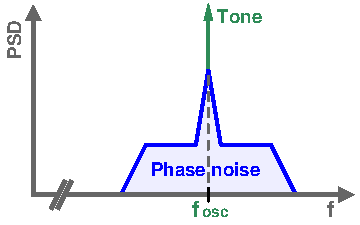
\includegraphics[width=0.5\textwidth, angle=0]{./figs/theory/phase_noise_psd}
		    \caption{Effect of phase noise on frequency tone.}
		    \label{fig:phase_noise_psd}
		\end{figure}

		\subsubsection{Relation to Power spectral density}\label{sec:pn_to_psd}
		An oscillator's voltage waveform can be described in terms of a phase trajectory function $\Phi_{osc}(t)$ and amplitude $A_0$ in the following manner (ignoring higher harmonics):
		\begin{equation}\label{eq:osc_wfm}
			V_{osc}(t) = \Re\left\{A_0e^{j\Phi_{osc}(t)}\right\}
		\end{equation}
		 In an oscillator, it is desirable for phase noise to be small, and zero mean ($\mathbb{E}[\Phi_{n}(t)]=0$). Using a constraint $\mathrm{Var}[\Phi_{n}(t)] << 1$ the following approximations can be applied to determine the oscillators spectral density in terms of the phase noise component $\Phi_n(t)$.
		\begin{align}
			V_{osc}(t) &= \Re\left\{A_0e^{j\omega_{osc}t}e^{j\Phi_{n}(t)}\right\} && \text{(oscillator waveform)} \\
			&= \Re\left\{A_0e^{j\omega_{osc}t}\sum_{k=0}^\infty\frac{(j\Phi_{n}(t))^k}{k!}\right\} && \text{(apply exponential Taylor series)} \\
			&\approx  \Re\left\{A_0e^{j\omega_{osc}t} +j\Phi_{n}(t)A_0e^{j\omega_{osc}t}\right\} && \text{(truncate series at k=1 given $\mathrm{Var}[\Phi_{n}(t)] << 1$)} \\
			&= A_0\cos(\omega_{osc}t) - \Phi_{n}(t)A_0\sin(\omega_{osc}t) &&\text{(taking real component)}\label{eq:pll_out_approx}\\
		\end{align}
		The result is a carrier cosine signal, and an orthogonal sine signal modulated by the phase noise $\Phi_{n}$. From this, the spectral density of the phase noise relative to the carrier can be estimated. The power spectral density $S_{V_{osc}}$ is computed in equations \ref{eq:psd_vout}-\ref{eq:psd_noise}. Due to orthogonality of the sine/cosine components of equation \ref{eq:pll_out_approx}, the cross terms that appear in the PSD computation are zero. 
		\begin{align}
			S_{V_{out}}(f) =& \lim_{\Delta T\rightarrow\infty}\frac{1}{\Delta T}|\mathcal{F}\{V_{out}(t)\cdot\mathrm{rect}(t/\Delta T)\}|^2 \label{eq:psd_vout}\\
			=&\lim_{\Delta T\rightarrow\infty}\frac{A_0^2}{\Delta T}|\mathcal{F}\{\cos(\omega_{osc}t)\cdot\mathrm{rect}(t/\Delta T)\}|^2 \label{eq:psd_carrier}\\ 
			&+ \lim_{\Delta T\rightarrow\infty}\frac{A_0^2}{\Delta T}|\mathcal{F}\{\Phi_{n}(t)\cdot\mathrm{rect}(t/\Delta T)\}*\mathcal{F}\{\sin(\omega_{osc}t)\cdot\mathrm{rect}(t/\Delta T)\}|^2 \label{eq:psd_noise}\\
		\end{align}
		 The noise power spectral density function of the output waveform $\mathcal{L}(\Delta f)$ is defined as the noise PSD at offset $\Delta f$ from the carrier frequency $f_{osc}$, normalized to the carrier power. Here the PSD of the carrier component is given by equation \ref{eq:psd_carrier}, and the noise component by equation \ref{eq:psd_noise}. Shifting equation \ref{eq:psd_noise} by $-\omega_{osc}$ and performing normalization for carrier power results in:
		\begin{equation}\label{eq:pn_psd_relation}
			\mathcal{L}(\Delta f) = \left.\lim_{\Delta T\rightarrow\infty}\frac{1}{\Delta T}|\mathcal{F}\{\Phi_{n}(t)\cdot\mathrm{rect}(t/\Delta T)\}|^2 \right|_{f=\Delta f}= S_{\Phi_{n}}(\Delta f)
		\end{equation}

		Thus, the noise PSD $\mathcal{L}(\Delta f)$ of the PLL output waveform relative to the carrier is equal to the PSD of the phase noise signal $\Phi_{n}(t)$, provided $\text{Var}[\Phi_{n}(t)] << 1$. The PSD of $\Phi_{n}(t)$ is notated as $S_{\Phi_{n}}(\Delta f)$.


	\subsubsection{Leeson's model}\label{dco_noise}
		Oscillator noise from thermal and stochastic sources is typical represented mathematically using Leeson's model for oscillator phase noise \cite{leeson_1966}. Leeson's model considers noise power density at an offset $\Delta f$ from the oscillator tone (carrier). Noise power density is represented with the function $\mathcal{L}(\Delta f)$, which is the noise power density normalized to the power of the oscillator carrier tone, in other words in units of dBc/Hz. Leeson's model divides phase noise into three regions, illustrated in figure \ref{fig:leeson_pn}: (1) flicker-noise dominated, with a slope of -30 dB/decade, (2) white frequency-noise dominated, with -20 dB per decade, and (3) a flat region, limited by the thermal noise floor or amplitude noise. It is noted that phase noise components are at frequencies different than the carrier, hence are orthogonal, and can be treated as independent components that are added to the main oscillator tone signal for analysis. 

			\begin{figure}[htb!]
		        \centering
		        \include{./figs/leeson_pn}
			    \caption{Phase noise regions of Leeson's model.}
			    \label{fig:leeson_pn}
			\end{figure}

		The equation for $\mathcal{L}(\Delta f)$ (from \cite{lee_hajimiri_2000}) is in equation \ref{eq:leesons}, and is dependent on temperature T, excess noise factor F, DC oscillator power $P_{DC}$, oscillator Q factor, and the transition frequencies $f_1$ and $f_2$ that separate the different noise regions. It is of interest to note that the phase noise relative to the carrier will increase as power decreases, which provides challenge for creating low power oscillators with acceptable phase noise characteristics. 
		\begin{equation}\label{eq:leesons}
		\mathcal{L}(\Delta f) = 10\log_{10}\left[\frac{2\text{F}k_B\text{T}}{P_{DC}}\left(1+\left(\frac{f_2}{2Q\Delta f}\right)^2\right)\left(1+\frac{f_1}{|\Delta f|}\right)\right] = S_{\Phi n_{DCO}}(\Delta f)
		\end{equation}
		For notational consistency, the following redefinition is used in the remainder of this paper: $S_{\Phi n_{DCO}}(f) = \mathcal{L}(\Delta f)|_{\Delta f = f}$

	\subsubsection{Phase Noise Figures of Merit}
	A common method to assign a figure of merit (FOM) to oscillator phase noise performance is to utilize the below relation \cite{Kinget1999}. Such a model assumes linear tradeoffs between power, frequency, and phase noise, and assumes that the rolloff of phase noise will occur with -20 dB/decade. A Lower FOM here is better.
	\begin{equation}\label{eq:fom_pn}
		\textnormal{FOM}_{\textnormal{pn}} = 10\log_{10}\left(\frac{P_{DC}}{\textnormal{1 mW}}\cdot\left(\frac{\Delta f}{f_0}\right)^2\right) + \mathcal{L}(\Delta f)
	\end{equation}
	Another FOM applied to PLLs is provided below, based on the RMS jitter of the PLL \cite{XiangGao2009}. Here, RMS jitter is used as the phase spectrum of a PLL is often more complicated than a simple oscillator, containing spurs, in-band phase noise supression, and peaking resulting from the PLL loop filter. It should be noted that RMS jitter (in time) is tied directly to total phase noise power, as expected by Parseval's theorem \cite{parseval_1799}.  Lower is better again with this FOM. 
	\begin{equation}\label{eq:fom_jitter}
		\textnormal{FOM}_{\textnormal{jitter}} = 10\log_{10}\left(\frac{\sigma_{t_j}^2}{(\textnormal{1 s})^2}\cdot\frac{P_{DC}}{\textnormal{1 mW}}\right)
	\end{equation}
	\begin{equation}
		\sigma_{t_j}^2 = \frac{\mathrm{Var}[\Phi_{n}(t)]}{\omega_0^2}
	\end{equation}
	In general, a good figure of merit is arrived to be decreasing power and/or minimizing total phase noise power. 
	
	\subsubsection{Ring Oscillator Phase Noise}\label{sec:ro_pn_limit}
	Oscillator phase noise for ring oscillators has a well defined limit as determined by analysis of noise of ideal RC circuits \cite{Navid2005}, which is provided in equation \ref{eq:ro_pn}. Note that this model is limited to analyzing the -20 dB/decade part of an oscillator's spectrum as seen by Leeson's model. 
	\begin{equation}\label{eq:ro_pn}
		\mathcal{L}_{min}(\Delta f)= 10\log 10\left(\frac{7.33k_BT}{P_{DC}}\left(\frac{f_0}{\Delta f}\right)^2\right)
	\end{equation}
	Applying this to the phase noise FOM equation \ref{eq:fom_pn}, a limit for ring oscillator phase noise FOM is determined in equation \ref{eq:ro_fom_limit}.
	\begin{equation}\label{eq:ro_fom_limit}
		\textnormal{FOM}_{\textnormal{pn,min}} = 10\log 10\left(7330k_BT\right)
	\end{equation}
	At 300K, it is expected that the jitter FOM for a ring oscillator should approach -165.2 dB. An example state of art comparison figure in \ref{fig:lc_ro_fom} shows clustering by oscillator type of jitter FOM calculated in various published works in \cite{Tohidian2015}. It is seen the FOM value calculated from theory is close to that seen implemented hardware.
	\begin{figure}[htb!]
		\center\includegraphics[width=1\textwidth, angle=0]{./figs/lc_ro_fom_comparison}
		\caption{FOM$_{jitter}$ of various LC and ring oscillators \cite{Tohidian2015}.}
		\label{fig:lc_ro_fom}
	\end{figure}

	\FloatBarrier



\subsection{PLL Phase Noise}\label{ntfs}
	Having an understanding of PLL theory, individual PLL component characteristics, and phase noise, a model for PLL phase noise can be constructed. To begin, noise sensitivity transfer functions are defined to refer each noise source to the PLL output. Here, all noise sources have been defined as additive signal components to each PLL component output. The full system noise model is in figure \ref{fig:full_pll_noise}.
	\begin{figure}[htb!]
		\center\fontfamily{\sfdefault}\selectfont
% XCircuit output "discrete_pll_full_noise.tex" for LaTeX input from discrete_pll_full_noise.ps
\def\putbox#1#2#3#4{\makebox[0.00000in][l]{\makebox[#1][l]{}\raisebox{\baselineskip}[0.00000in][0.00000in]{\raisebox{#2}[0.00000in][0.00000in]{\scalebox{#3}{#4}}}}}
\def\rightbox#1{\makebox[0.00000in][r]{#1}}
\def\centbox#1{\makebox[0.00000in]{#1}}
\def\topbox#1{\raisebox{-0.60\baselineskip}[0.00000in][0.00000in]{#1}}
\def\midbox#1{\raisebox{-0.20\baselineskip}[0.00000in][0.00000in]{#1}}
   \scalebox{1}{
   \normalsize
   \parbox{6.30000in}{
   \includegraphics[scale=0.60000]{./figs/discrete_pll_full_noise.pdf}\\
   % translate x=416 y=544 scale 0.38
   \putbox{0.33600in}{1.00800in}{0.84}{$\Phi_{ref}$(t)}%
   \putbox{1.56000in}{0.51000in}{0.84}{$\Phi_{div}$(t)}%
   \putbox{2.27400in}{1.03200in}{0.84}{e$_\Phi$(t)}%
   \putbox{1.42200in}{1.08600in}{0.84}{\rotatebox{-360}{$K_{PD}$}}%
   \putbox{1.20600in}{1.00800in}{0.84}{$\Phi_e$}%
   \putbox{0.83400in}{1.28400in}{0.84}{PD}%
   \putbox{2.77200in}{0.89400in}{0.84}{H$_{LF}$(s)}%
   \putbox{3.79800in}{1.02000in}{0.84}{u(t)}%
   \putbox{4.26000in}{0.90600in}{0.84}{$\frac{2\pi K_{DCO}}{s}$}%
   \putbox{5.22000in}{0.99600in}{0.84}{$\Phi_{out}$(t)}%
   \putbox{3.22200in}{0.39600in}{0.84}{$\div$ N}%
   \putbox{4.13400in}{1.17000in}{0.84}{DCO}%
   \putbox{1.93200in}{1.30800in}{0.84}{q$_{n_{PD}}$(t)}%
   \putbox{3.57000in}{1.30800in}{0.84}{\rotatebox{-360}{q$_{n_{LF}}$(t)}}%
   \putbox{2.82000in}{0.09600in}{0.84}{$\Phi_{n_{div}}$(t)}%
   \putbox{5.12400in}{1.30800in}{0.84}{$\Phi_{n_{DCO}}$(t)}%
   } % close 'parbox'
   } % close 'scalebox'
   \vspace{-\baselineskip} % this is not necessary, but looks better
\fontfamily{\rmdefault}\selectfont

		\caption{Full PLL additive noise model.}
		\label{fig:full_pll_noise}
	\end{figure}
	\FloatBarrier
	\subsubsection{PLL Noise Transfer Functions}
	Following the approach of \cite{perrott_2002}, a transfer function $\hat{\mathrm{T}}(s)$ is defined in equation \ref{eq:parameterizing_tf} which characterizes the normalized closed loop phase response from reference input to output of the PLL. $L(s)$ is the PLL loop gain and $T(s)$ is the PLL closed loop transfer function. 
	\begin{equation}\label{eq:parameterizing_tf}
	\hat{\mathrm{T}}(s) = \frac{\mathrm{L}(s)}{1+\mathrm{L}(s)}\hspace{1em} \text{s.t.} \hspace{1em} \mathrm{T}(s) = \frac{\Phi_{out}}{\Phi_{ref}} = \mathrm{N}\hat{\mathrm{T}}(s) 
	\end{equation}
	Solving for the closed transfer functions between each noise source ($q_{n_{BBPD}}$, $q_{n_{LF}}$, $\Phi_{n_{DCO}}$ and $\Phi_{n_{div}}$) to the output $\Phi_{out}$ in the s-domain yields equations \ref{eq:noise_tf_tdc}-\ref{eq:noise_tf_div}.
	\begin{align}
		\frac{\Phi_{out}(s)}{q_{n_{PD}}(s)} & = \frac{2\pi\frac{K_{DCO}}{s}\mathrm{H}_{LF}(s)}{1+\mathrm{L}(s)}= \frac{\mathrm{N}}{\mathrm{K_{PD}}}\frac{\mathrm{L}(s)}{1+\mathrm{L}(s)} = \frac{\mathrm{N}}{\mathrm{K_{PD}}}\hat{\mathrm{T}}(s)\label{eq:noise_tf_tdc}\\
		\frac{\Phi_{out}(s)}{\Phi_{n_{DCO}}(s)} & = \frac{1}{1+\mathrm{L}(s)}= 1-\hat{\mathrm{T}}(s)\\
		\frac{\Phi_{out}(s)}{q_{n_{LF}}(s)} & = \frac{2\pi\frac{K_{DCO}}{s}}{1+\mathrm{L}(s)} = 2\pi\frac{K_{DCO}}{s}(1-\hat{\mathrm{T}}(s))\\
		\frac{\Phi_{out}(s)}{\Phi_{n_{div}}(s)} & =\frac{K_{BBPD} 2\pi \frac{K_{DCO}}{s}\mathrm{H}_{LF}(s)}{1+\mathrm{L}(s)}= \mathrm{N}\frac{\mathrm{L}(s)}{1+\mathrm{L}(s)} = \mathrm{N}\hat{\mathrm{T}}(s)\label{eq:noise_tf_div}
	\end{align}

	\subsubsection{PLL Output-referred Noise}\label{sec:pll_output_noise}
		Using the noise transfer functions, the expressions for noise power spectrum of the BBPD (equation \ref{eq:bbpd_noise_psd}) and the noise spectrum of a ring oscillator (equation \ref{eq:ro_pn}), the PLL output phase noise spectrum of each component is determined by multiplying the magnitude squared of each noise transfer function with the respective noise spectral density. Here it is found that the BBPD noise component out of the PLL is given in equation \ref{eq:out_psd_bbpd_pll}, and the oscillator component is given in equation \ref{eq:out_psd_dco_pll}. The loop filter and divider components are here ignored, as they will be shown not be relevant in this work. 

		% \begin{equation}\label{eq:bbpd_noise_psd}
		% 	S_{ n_{BBPD}(f)} = \frac{\sigma_{n_{BBPD}}^2}{\Delta f} = \frac{\left(1-\frac{2}{\pi}\right)}{f_{ref}}
		% \end{equation}
			% \begin{align}\label{eq:cl_bbpd_pll}
			% 	\mathrm{T}(s)=\frac{\Phi_{out}(s)}{\Phi_{ref}(s)} = \frac{2\pi \sqrt{\frac{2}{\pi}}\frac{1}{\sigma_{\Phi_e}}K_{DCO}\sum_{j=0}^Z b_js^j}{\sum_{k=0}^P a_ks^{k+1} + 2\pi \sqrt{\frac{2}{\pi}}\frac{\mathrm{1}}{\sigma_{\Phi_e}\mathrm{N}}K_{DCO}\sum_{j=0}^Z b_js^j} = \mathrm{N}\frac{\mathrm{L}(s)}{1+\mathrm{L}(s)}
			% \end{align}
		% \begin{align}\label{eq:ntf_bbpd_pll}
		% 	\frac{\Phi_{out}(f)}{q_{n_{{BBPD}}}(f)} = \sqrt{\frac{\pi}{2}}\sigma_{\Phi_e}\mathrm{N}\frac{\mathrm{L}(f)}{1+\mathrm{L}(f)} = \sqrt{\frac{\pi}{2}}\sigma_{\Phi_e}\mathrm{N}\hat{\mathrm{T}}(f)
		% \end{align}
		\begin{align}\label{eq:out_psd_bbpd_pll}
			S_{\Phi n_{BBPD,out}}(f) &= S_{n_{BBPD}}(f)\left|\frac{\Phi_{out}(f)}{q_{n_{BBPD}}(f)}\right|^2 = \frac{\left(\frac{\pi}{2}-1\right)}{f_{ref}}\left|\sigma_{\Phi_e}\mathrm{N}\hat{\mathrm{T}}(f)\right|^2
		\end{align}
		\begin{align}\label{eq:out_psd_dco_pll}
			S_{\Phi n_{DCO,out}}(f) &= \mathcal{L}_{min}(f)\left|\frac{\Phi_{out}(f)}{q_{n_{DCO}}(f)}\right|^2 = \frac{7.33k_BT}{P}\left(\frac{f_0}{f}\right)^2|1-\hat{\textnormal{T}}(f)|^2 
		\end{align}
		The total output noise power spectral density is given as the sum of the components, presuming independence of all noise sources. Following the results of section \ref{sec:pn_to_psd}, which determined that oscillator power spectrum is equivalent to the phase noise power spectrum for zero mean phase noise with low power, the final oscillator power spectrum at $\Delta f$ from the carrier is in equation \ref{eq:pll_noise_psd}.
		\begin{align}
			S_{n_{PLL}}(f_{osc} + \Delta f) &= S_{\Phi n_{BBPD,out}}(\Delta f) + S_{\Phi n_{DCO,out}}(\Delta f)\label{eq:pll_noise_psd}\\
			&= \frac{\left(\frac{\pi}{2}-1\right)}{f_{ref}}\left|\sigma_{\Phi_e}\mathrm{N}\hat{\mathrm{T}}(\Delta f)\right|^2 + \frac{7.33k_BT}{P}\left(\frac{f_0}{\Delta f}\right)^2|1-\hat{\textnormal{T}}({\Delta f})|^2
		\end{align}
		A complexity arises in equation \ref{eq:pll_noise_psd} due to the fact that the power spectum is a function of the root mean squared (RMS) phase error, $\sigma_{\Phi_e}$. $\sigma_{\Phi_e}$ may be calculated as equation \ref{eq:rpm}. It is seen that the spectrum and $\sigma_{\Phi_e}$ are cyclically defined, so a system of equations formed by the two must be solved to determine the final noise spectrum.

		\begin{equation}\label{eq:rpm}
			\sigma_{\Phi_e} = \sqrt{2\int_0^\infty S_{n_{PLL}}(f_{osc} + \Delta f)d\Delta f}
		\end{equation}

	% \subsubsection{Phase Noise Optimization}\label{bbpd_theory}
	% 	From this author's previous work \cite{Me}, it has been shown that total phase noise power (equivalently jitter) is optimizable with in a BBPD-based PLL, specifically when using a proportional-integral (PI) filter based controller. It is observed that as the loop filter bandwidth is varied, the phase noise contributions will be varied also in accordance to the transfer functions determined in section \ref{sec:pll_output_noise}. Specifically, it is seen the TDC noise power contribution grows monotonically with bandwidth, while the oscillator contribution decreases with increasing bandwidth. This effect is exhibited in figure \ref{fig:bw_vs_pn2}. Thus, a point of optimality exists for loop bandwidth where the total noise power is at a minimum. Figure \ref{fig:pll_pn_opt_ex} shows the result of a simulated BBPD PLL with PI-loop filter controller, whose bandwidth is varied. It is seen that there is infact a convex optimal point for phase noise in terms of PLL bandwidth.
	% 	\begin{figure}[htb!]
	% 		\center\includegraphics[width=1\textwidth, angle=0]{figs/theory/loop_bandwidth}
	% 		\caption{Bandwidth versus total integrated phase noise of PLL.}
	% 		\label{fig:bw_vs_pn2}
	% 	\end{figure}
	% 	\begin{figure}[htb!]
	%         \centering
	%         \includegraphics[width=0.6\textwidth, angle=0]{figs/bandwidth_vs_pn.pdf}
	% 	    \caption{Integrated phase noise power versus bandwidth for the same PLL.}
	% 	    \label{fig:pll_pn_opt_ex}
	% 	\end{figure}
\FloatBarrier{\color{white}.}


\pagebreak
\section{Redefining Requirements}
\hl{I've decided to have problem description state radio requirements of intended system, and then here I will derive the requirement for CNR of the PLL to meet those radio requirements from a BER vs CNR simulation. }
The requirements imposed on this PLL are defined in terms of a radio system for which it will be a component of. First, the modulation scheme of this system is described. Gaussian frequency shift keying with bandwidth-time (BT) product of 0.3 is utilized as the basic scheme, With a nominal bit rate of 1 Mbps. Under such circumstances, 1 and 0 are respectively encoded as $\pm$250 kHz of frequency deviation from the carrier. In order to improve bit error rate, while mantaining compatability with 1 Mbps tramsitters, a modified data rate of 250 ksymbols/s is used where one data symbol \hl{WIP... skip this for now.}
	% \input{theory2.tex}
	% \section{Methods}\label{methods}
	\FloatBarrier\newpage
	\section{Design}\label{design}
	% The methods for implementation of a behavioral, discrete-time PLL simulator and for the PLL loop filter automation and optimization will be covered here.

% \hl{Talk about how simulator is implemented:}
% \hl{Discrete simulation models of phase noise, dco etc}
% \hl{Filter optimization}
% \hl{-phase noise and lock time estimate in frequency domain}
The primary objective in this work is to obtain a very low $100\mu$W power consumption for a 2.448 GHz PLL frequency synthesizer, while achieving a carrier-to-noise ratio for the synthesized signal of $>$20 dB. Consequently, the design philosophy adhered to in this work is pursue simplicity wherever possible, in order to reduce number of sources of power draw and noise. Furthermore, this design is targeted to allow duty cycled operation to further reduce power. Thus, an all-digital architecture has been selected to enable the possibility to save the PLL state, enter an ultra-low-power sleep state, and then resume from the stored state rapidly, without requiring relocking of the PLL. 

\subsection{Proposed Architecture - ADPLL}\label{pll_arch}
			\begin{figure}[htb!]
		        \centering
		        \includegraphics[width=1\textwidth, angle=0]{./figs/design/pll_master_arch_final}
			    \caption{ADPLL Architecture.}
			    \label{fig:pll_arch}
			\end{figure}
	The undertaken PLL architecture is in figure \ref{fig:pll_arch}. It comprises primarily of five components: (1) counter-based phase detector for initial start up, (2) bang-bang phase detector for steady state feedback, (3) proportional-integral controller loop filter, (4) DCO implemented as a VCO plus capacitive DACs, and (5) a control and calibration engine, consisting of digital logic. This design was achieved via minimization of complexity. First, the need of a divider is removed from the design by the usage of both the counter phase detector and BBPD. For initial cold start up of the PLL from an unknown state, the counter-based phase detector functions as a low-resolution replacement for a divider and linear phase detector. When near steady state, the counter-PD is disabled and replaced by BBPD feedback, which will maintain the PLL at steady state. The removal of a divider results in lower power consumption, and less noise added in-loop. The usage of only a BBPD in steady state further reduces power, as it is a minimum complexity phase detector. This is expected without significant performance degredation, as with proper optimization, BBPD PLLs can obtain comparable perform to linear charge-pump style PLLs \cite{xu_abidi_2017}. Additional power improvements are obtained in the usage of digital logic to implement the loop filter, using a simple PI-controller architecture. The final power saving move is implemented in a DCO based on the combination of several CDACs with a voltage controlled ring oscillator. This reduces to near zero the static curent draw associated with control of the VCO. The overall design is implemented with no static current paths, other than that associated with leakage, achieved by favoring static logic derived components throughout the PLL.


	A further feature gained in the proposed all-digital architecture is the ability to abruptly save the state of the PLL digitally and place it into an ultra low power sleep mode, and then later resume the PLL from the saved state. Figure \ref{fig:pll_sleep} demonstrate such operation, where $t_{l1}$ is the lock time from cold start, and $t_{l2}$ is the time to relock from a resume. This functionality enables the ability to rapidly duty cycle the PLL between active and sleep states, with minimal time to relock. Power consumption of the PLL is reduced by a factor that is the duty cycle which it is operated, and in this design can enable as low as 1$\mu$W power consumption as 1\% duty cycle. 

			\begin{figure}[htb!]
			        \centering
			        \includegraphics[width=0.6\textwidth, angle=0]{./figs/design/pll_sleep}
			    \caption{PLL sleep and resume operation.}
			    \label{fig:pll_sleep}
			\end{figure}


% \vspace{-2em}
% \begin{figure}[htb!]
% 	\center\include{./figs/tdc_bbpll}
% 	\caption{PLL with parallel bang-bang phase detector and TDC.}
% 	\label{fig:tdc_bbpll}
% \end{figure}

The proposed digital architecture also enables a form of fast-locking via gear switching of the loop filter \cite{staszewski_balsara_2007}. In this work, the counter-based TDC is initially used for large frequency and phase errors with a loop filter optimized for speed, which after locking can be changed (gear-switched) to a BBPD optimized loop filter chosen to minimize total phase-noise. Design of optimal filters will be discused later on.

	
	\subsubsection{Power budget}
	The below power budget was used in the design process to divide up the 100 $\mu$W allotment between the different PLL components. In order to minimize oscillator phase noise, as large of a portion was allotted to the oscillator, being 80\%. 
		\begin{table}[htb!]
			\centering
			\def\arraystretch{1.5}		
			\setlength\arrayrulewidth{0.75pt}
			\setlength{\tabcolsep}{1em} % for the horizontal padding
			\begin{tabular}{|c|c|c|c|c|}
				\hline 
				\rule[-1ex]{0pt}{2.5ex} \cellcolor{gray!40}\textbf{DCO} & \cellcolor{gray!40}\textbf{Phase detector} & \cellcolor{gray!40}\textbf{Digital (LF)}& \cellcolor{gray!40}\textbf{Other} & \cellcolor{gray!40}\textbf{SUM} \\ 
				\hline 
				\rule[-1ex]{0pt}{2.5ex} 80 $\mu$W& 10 $\mu$W &  10 $\mu$W  & 0 $ \mu$W & $\leq$ 100  $\mu$W\\ 
				\hline 
			\end{tabular} 
			% \caption{Assigned specifications for branch line hybrid design.}
			% \label{asgn_specs}
		\end{table}   



	\subsubsection{Floorplan}
	The below floor plan (dimensions in microns) has been devised to meet the area requirement of $<$ 0.01 mm$^2$.
		\begin{figure}[htb!]
	        \centering
	        \includegraphics[width=0.6\textwidth, angle=0]{./figs/pll_floorplan2}
		    \caption{PLL floorplan.}
		\end{figure}

\subsubsection{Dividerless PLL}
\vspace{-2em}
\begin{figure}[htb!]
	\center\fontfamily{\sfdefault}\selectfont
% XCircuit output "bbpll_full_noise.tex" for LaTeX input from bbpll_full_noise.ps
\def\putbox#1#2#3#4{\makebox[0.00000in][l]{\makebox[#1][l]{}\raisebox{\baselineskip}[0.00000in][0.00000in]{\raisebox{#2}[0.00000in][0.00000in]{\scalebox{#3}{#4}}}}}
\def\rightbox#1{\makebox[0.00000in][r]{#1}}
\def\centbox#1{\makebox[0.00000in]{#1}}
\def\topbox#1{\raisebox{-0.60\baselineskip}[0.00000in][0.00000in]{#1}}
\def\midbox#1{\raisebox{-0.20\baselineskip}[0.00000in][0.00000in]{#1}}
   \scalebox{1}{
   \normalsize
   \parbox{5.50000in}{
   \includegraphics[scale=0.60000]{./figs/bbpll_full_noise.pdf}\\
   % translate x=416 y=448 scale 0.38
   \putbox{0.33600in}{0.70800in}{0.84}{$\Phi_{ref}$(t)}%
   \putbox{2.27400in}{0.73200in}{0.84}{e$_\Phi$(t)}%
   \putbox{1.42200in}{0.78600in}{0.84}{\rotatebox{-360}{$K_{BBPD}$}}%
   \putbox{1.20600in}{0.70800in}{0.84}{$\Phi_e$}%
   \putbox{0.83400in}{0.98400in}{0.84}{BBPD}%
   \putbox{2.77200in}{0.59400in}{0.84}{H$_{LF}$(s)}%
   \putbox{3.39600in}{0.72000in}{0.84}{u(t)}%
   \putbox{3.85800in}{0.60600in}{0.84}{$\frac{2\pi K_{DCO}}{s}$}%
   \putbox{4.82400in}{0.69600in}{0.84}{$\Phi_{out}$(t)}%
   \putbox{3.73200in}{0.87000in}{0.84}{DCO}%
   \putbox{1.93200in}{1.00800in}{0.84}{q$_{n_{BBPD}}$(t)}%
   \putbox{4.72200in}{1.00800in}{0.84}{$\Phi_{n_{DCO}}$(t)}%
   } % close 'parbox'
   } % close 'scalebox'
   \vspace{-\baselineskip} % this is not necessary, but looks better
\fontfamily{\rmdefault}\selectfont

	\caption{BBPD-PLL full noise model.}
	\label{fig:bbpll_full_noise}
\end{figure}

In the PLL theory (section \ref{sec:pll_output_noise}), the derived PLL detector phase noise component (equation \ref{eq:out_psd_bbpd_pll}) contains a term proportional to $N^2$, that is the detector noise will grow with the square of the PLL divider ratio. It is, however, possible to remove this $N^2$ dependency by usage of oscillator sub-sampling within the PLL \cite{Gao2015}. This is achieved by directly sampling the PLL output at a rate equivalent to the reference frequency. This is equivalent to removing the divider from the PLL loop and directly connecting the PLL output to the phase detector, which has been employed in this work (see figure \ref{fig:pll_arch}). To lock to the desired frequency, though, it must be guaranteed that the PLL frequency at the start of sub-sampling operation be within $f_{ref}/2$ of the target frequency (the PLL will lock to the nearest multiple of the reference frequency). In this work, this is achieved through sequencing at startup through two phase detectors. A synchronous counter phase detector (which emulates both a divider and phase detector) initially locks the PLL within $f_{ref}/2$ of the target frequency, after which the PLL is operated in sub-sampling bang-bang phase detector.

  In accordance to the change to a dividerless operation, the PLL closed loop transfer function has been rederived in equation \ref{eq:cont_pll_tf2}. Furthermore, new expressions for PLL output phase noise with a BBPD is given in equation \ref{eq:out_psd_bbpd_pll2}, and PLL output oscillator noise with a ring oscillator is given in equation \ref{eq:out_psd_dco_pll2}, for the noise model in figure \ref{fig:bbpll_full_noise}. Noise due to the loop filter here is ignored, as it will be possible to adjust the loop filter datapath resolution to make digital quantizaiton noise effects negligible.
		\begin{align} \label{eq:cont_pll_tf2}
			\mathrm{T}(s) = \frac{\Phi_{out}(s)}{\Phi_{ref}(s)} = \frac{2\pi K_{BBPD}K_{DCO}\sum_{j=0}^Z b_js^j}{\sum_{k=0}^P a_ks^{k+1} + 2\pi K_{BBPD}K_{DCO}\sum_{j=0}^Z b_js^j} = \frac{\mathrm{L}(s)}{1 + \mathrm{L}(s)}
		\end{align}
		\begin{align}\label{eq:out_psd_bbpd_pll2}
			S_{\Phi n_{BBPD,out}}(f) &= S_{n_{BBPD}}(f)\left|\frac{\Phi_{out}(f)}{q_{n_{BBPD}}(f)}\right|^2 = \frac{\left(\frac{\pi}{2}-1\right)}{f_{ref}}\left|\sigma_{\Phi_e}\mathrm{T}(f)\right|^2
		\end{align}
		\begin{align}\label{eq:out_psd_dco_pll2}
			S_{\Phi n_{DCO,out}}(f) &= \mathcal{L}_{min}(f)\left|\frac{\Phi_{out}(f)}{q_{n_{DCO}}(f)}\right|^2 = \frac{7.33k_BT}{P}\left(\frac{f_0}{f}\right)^2|1-\textnormal{T}(f)|^2 
		\end{align}

% ################################################################################################
% ################################################################################################
	\subsection{Bang-Bang Phase Detector}
		A bang-bang phase detector, as introduced in section \ref{bbpd_theory}, can be implemented physically with a D flip-flop \cite{Razavi2020} and logic to map the logical state to a signed $\pm$1 value that may be passed into a digital loop filter. This is shown in figure \ref{fig:bbpd_dff}. 

		\begin{figure}[htb!]
			\center\includegraphics[width=0.4\textwidth, angle=0]{./figs/design/bbpd_}
			\caption{Bang-bang phase detector with D flip-flop.}
			\label{fig:bbpd_dff}
		\end{figure}
		The realization of a BBPD using a digital flip flop introduces additional noise to the system in the form of jitter. Jitter arises as an artifact of circuit and supply noise. For small time differentials between the BBPD inputs X and Y, the output can be stochatically corrupted due to the presence of noise. Furthermore, physical D flip flop implementations exhibit set-up and hold time requirements for data to be stable (to allow internal nodes to settle), so deterministic corruption of phase detection can be imparted if the inputs violate physical timing requirements. These sources of corruption cause BB-PD transfer characteristics in terms of output expectation, $\mathbb{E}[Z]$, with respect to input timing difference $\Delta t_{XY}$ to deviate from an ideal step response, demonstrated in figure \ref{fig:bbpd_jit_pdf}. Analytically, the corruption of the transfer characteristic can be viewed as being caused by an additive phase noise component before the signum operation in the BBPD, as shown in figure \ref{fig:bbpd_noise_nonlinear}. The expectation $\mathbb{E}[Z(\Delta t_{XY})]$ acts as a cumulative distribution function (CDF) for this phase noise component. Thus, differentiation of $\mathbb{E}[Z(\Delta t_{XY})]$ results in a probability distribution function (PDF) P(T=$\Delta t_{xy}$) of this phase noise signal. Statistical analysis of variance of the PDF provides an RMS value for timing jitter of this additive noise source, $\sqrt{\mathrm{Var}[T]} = \sigma_{t,j}$. The RMS timing jitter may be converted to RMS phase error of the noise source as $\sigma_{\Phi_j} = 2\pi f_{osc}\sigma_{t_j}$. This analysis approach is applied in this work to evaluate BBPD performance.
 
		\begin{figure}[htb!]
		    \centering
			\includegraphics[width=0.6\textwidth, angle=0]{./figs/bbpd_jitter.pdf}
			\caption{BBPD output expectation and jitter PDF versus input time differential.}
			\label{fig:bbpd_jit_pdf}
		\end{figure}

	\begin{figure}[htb!]
	    \centering
	    \begin{subfigure}{0.5\textwidth}
	        \centering
	        \includegraphics[width=0.8\textwidth, angle=0]{figs/design/bbpd_noise_nonlinear}
	        \caption{ }
	        \label{fig:bbpd_noise_nonlinear}
	    \end{subfigure}%
	    \begin{subfigure}{0.5\textwidth}
	        \centering
	        \includegraphics[width=0.9\textwidth, angle=0]{figs/design/bbpd_noise_linear}
	        \caption{ }
	        \label{fig:bbpd_noise_linear}
	    \end{subfigure}
	    % \caption{x.}
	    \caption{\textbf{(a)} Noisy BBPD nonlinear model \textbf{(b)} Noisy BBPD linearized model}
	     \label{fig:bbpd_noisy}
	\end{figure} 

	With a model for BBPD noise due to implementation non-idealities, a modified linearized model for the BBPD will be established here. This model will reconcile the ideal BBPD noise introduced in section \ref{sec:bbpd_noise} with the noise due to the new additive jitter component just described. First, a component representing the non-ideal jitter component, $\Phi_j$, is added into noise model from figure \ref{fig:bbpll_full_noise}. The result is the linearized model of figure \ref{fig:bbpd_noise_linear}. We then define a modified phase error, $\hat{\Phi}_e$, which includes the nominal $\Phi_e$ and the jitter corruption:
	\begin{equation}
	\hat{\Phi}_e = \Phi_e + \Phi_j.
	\end{equation}
	$\hat{\Phi}_e$ has a variance defined as $\sigma_{\hat{\Phi}_e}^2 = \sigma_{\Phi_e}^2 + \sigma_{\Phi_j}^2$, assuming $\Phi_e$ and $\Phi_j$ are uncorrelated. Defining BBPD gain in terms of $\sigma_{\hat{\Phi}_e}$:
	\begin{equation}
		K_{BBPD} = \sqrt{\frac{2}{\pi}}\cdot\frac{1}{\sigma_{\hat{\Phi}_e}} = \sqrt{\frac{2}{\pi}}\cdot\frac{1}{\sqrt{\sigma_{\Phi_e}^2 + \sigma_{\Phi_j}^2}}
	\end{equation}

	 It is then observed that the output Z is valued $\pm$1, thus its power is always $\sigma_Z^2$=1. Furthermore:
	\begin{equation}
	 	\sigma^2_{Z} = 1 = K_{BBPD}^2(\sigma^2_{\phi_e} +\sigma^2_{\phi_j})  + \sigma^2_{q_{n,BBPD}}
	\end{equation}
	 As determined in section \ref{sec:bbpd_noise}, it is inherent that $\sigma^2_{q_{n,BBPD}} = 1 - \frac{2}{\pi}$. If the total output noise
			\begin{equation}
				\sigma^2_{\phi_{n,BBPD}} =  \sigma^2_{q_{n,BBPD}} + K_{BBPD}^2\sigma^2_{\phi_j} =  1 - \frac{2}{\pi}\frac{\sigma^2_{\phi_e}}{\sigma^2_{\phi_j} + \sigma^2_{\phi_e}}
			\end{equation}
	If the BB-PD is connected directly to oscillator output, $\sigma^2_{\phi_e}$ = $\sigma^2_{\phi_n}$, i.e. the PLL output phase noise. The spectral density of the BB-PD phase noise is then:
		\begin{equation}
			S_{\phi_{n,BBPD}} = \frac{\sigma^2_{\phi_{n,BBPD}}}{f_{ref}} =  \frac{1 - \frac{2}{\pi}\frac{\sigma^2_{\phi_n}}{\sigma^2_{\phi_j} + \sigma^2_{\phi_n}}}{f_{ref}}
		\end{equation}

		\begin{align}\label{eq:out_psd_bbpd_pll3}
			S_{\Phi n_{BBPD,out}}(f) &= S_{n_{BBPD}}(f)\left|\frac{\Phi_{out}(f)}{q_{n_{BBPD}}(f)}\right|^2 = \frac{\frac{\pi}{2}(\sigma^2_{\phi_j} + \sigma^2_{\phi_n})-\sigma^2_{\phi_n}}{f_{ref}}\left|\mathrm{T}(f)\right|^2
		\end{align}

	% \begin{itemize}[itemsep=4pt,label=\protect---]
	% 	\item It is observed that PLL phase noise spectrum is approximately Lorentzian (except for peaking and flicker noise components). Given BB-PD noise PSD of $S_{\phi_{n,BBPD}}$, and an oscillator with noise PSD $S_{\phi_{n,osc}}(\Delta f)$, the optimal bandwidth for minimum noise power is:

	% 	\begin{equation}
	% 		BW_{opt} =  \sqrt{\frac{S_{\phi_{n,osc}}(\Delta f)}{S_{\phi_{n,BBPD}}}}\Delta f
	% 	\end{equation}
	% 	\item The total PLL output phase noise with optimal bandwidth is then:

	% 	\begin{equation}
	% 		\sigma^2_{\phi_{n,opt}} =   \pi\sqrt{\phi_{n,osc}(\Delta f)S_{\phi_{n,BBPD}}}\Delta f
	% 	\end{equation}
	% \end{itemize}
	% \vspace{-3em}
	% \begin{figure}[htb!]
	%     \centering
	%     \begin{subfigure}{0.33\textwidth}
	%         \centering
	%         \includegraphics[width=1\textwidth, angle=0]{./figs/pll_spectrum_lorentzian.pdf}
	%     \end{subfigure}%
	%     \begin{subfigure}{0.33\textwidth}
	%         \centering
	%         \center\includegraphics[width=1.0\textwidth, angle=0]{./figs/bandwidth_vs_pn.pdf}
	%     \end{subfigure}
	%     % \caption{Approximate model for ring oscillator inverter delay cell.}
	% \end{figure}




	% \begin{itemize}[itemsep=4pt,label=\protect---]
	% 	\item Using the findings for BB-PD noise PSD, assumption of Lorentzian spectrum, and constraint that BW = $\alpha f_{ref}$ (recommended $\alpha$$<$0.1 [2], rule of thumb since ancient PLL days). Given oscillator center frequency $f_c$, BB-PD jitter is constrained:

	% 	\begin{equation}
	% 		\sigma_{t_j} \leq \frac{\sigma_{\Phi_n}}{2\pi f_c}\sqrt{\frac{2}{\pi}\left(\frac{1}{\pi\alpha} - \frac{\pi}{2} + 1\right)} = \frac{\sigma_{\Phi_n}}{2\pi f_c}\beta(\alpha)
	% 	\end{equation}
	% 	\item $\beta(\alpha=0.1)$ = 1.28, $\beta(\alpha=0.05)$ = 1.92.
	% 	\item Using my PLL specifications ($f_c$ = 2.448 GHz, CNR = -$\sigma_{\Phi_n}$ = 17 dB, $\alpha=0.1$), {\color{red}\textbf{$\sigma_{t,j}\leq 11.8 $ ps}}
	% \end{itemize}



	% \begin{itemize}[itemsep=4pt,label=\protect---]
	% 	\item With an unconstrained relationship for BW and $f_{ref}$, and the optimal bandwidth finding, it is determined that the optimal value of $\sigma_{t,j}$ for minimum phase noise is:

	% 	\begin{equation}
	% 		\sigma_{t_j,opt} = \frac{\sigma_{\Phi_n}}{2\pi f_c}\sqrt{\frac{2}{\pi}\left[\frac{\sigma^4_{\Phi_n} f_{ref}}{\pi^2 S_{\phi_{n,osc}}(\Delta f) \Delta f^2} - \left(\frac{\pi}{2} - 1\right)\sigma^2_{\Phi_n}\right]}
	% 	\end{equation}

	% \end{itemize}

	% \begin{itemize}[itemsep=4pt,label=\protect---]
	% 	\item Setting the two jitter equations of the last side equal, it is found that optimal phase noise power is:

	% 	\begin{equation}
	% 		\sigma^2_{\Phi_n, opt} = \frac{\pi S_{\phi_{n,osc}}(\Delta f) \Delta f^2}{\alpha f_{ref}}
	% 	\end{equation}
	% 	\item The optimal reference frequency ($\sigma_{\Phi_n}=2\pi f_c \sigma_{t_n}$ = CNR):
	% 	\begin{equation}
	% 		f_{ref} = \frac{\pi S_{\phi_{n,osc}}(\Delta f) \Delta f^2}{\alpha \sigma^2_{\Phi_n}}
	% 	\end{equation}
	% 	\item The optimal oscillator phase noise at offset $\Delta f$:
	% 	\begin{equation}
	% 		S_{\phi_{n,osc}}(\Delta f) = \frac{\alpha f_{ref}\sigma^2_{\Phi_n}}{\pi \Delta f^2} 
	% 	\end{equation}
	% 	\item For CNR = 17 dB, $S_{\phi_{n,osc}}(\Delta f = 1 MHz)$ = -80 dBc/Hz, $\alpha$ = 0.1, {\color{red}the optimal $f_{ref}$ = 15.7 MHz.}
	% 	\item For CNR = 20 dB, $S_{\phi_{n,osc}}(\Delta f = 1 MHz)$ = -80 dBc/Hz, $\alpha$ = 0.1, {\color{red}the optimal $f_{ref}$ = 31.4 MHz.}
	% \end{itemize}


		\FloatBarrier






		\subsubsection{Circuit}
		The physcial implementation of the bang-bang phase detector has been selected to utilize a true single phase clock (TSPC) D-flip flop \cite{Yuan1989}. The positive-edge triggered variant of this circuit has been implemented as shown in figure \ref{fig:tspc_dff}. Selection of this topology was based on the desire for the usage of a single ended clock as a reference signal.

			\begin{figure}[htb!]
			        \centering
			        \includegraphics[width=0.6\textwidth, angle=0]{./figs/design/tspc_}
			    \caption{True single-phase clock (TSPC) D flip-flop, positive edge triggered.}
			    \label{fig:tspc_dff}
			\end{figure}

		This TSPC design was validated in simulation with RVT devices with all devices set with (W/L) = \{100n/20n, 200n/20n\}, and with supply voltages of 0.5 and 0.8 volts. Results for jitter PDF are in figure \ref{fig:tspc_dff_sim}, and the RMS jitter and power consumption are in table \ref{tab:dff}. For implementation (W/L) = 100n/20n was selected for all devices, as to ensure that the budgeted power of 10 $\mu$W is met with layout parasitics. 


		% \end{itemize}
		% % \vspace{-3em}
		% \begin{figure}[htb!]
		%     \centering
		%     \begin{subfigure}{0.5\textwidth}
		%         \centering
		%         \includegraphics[width=0.8\textwidth, angle=0]{./figs/tspc_dff.pdf}
		%         \caption{TSPC DFF}
		%     \end{subfigure}%
		%     \begin{subfigure}{0.5\textwidth}
		%         \centering
		%         \center\includegraphics[width=0.8\textwidth, angle=0]{./figs/etspc_dff.pdf}
		%         \caption{e-TSPC DFF}
		%     \end{subfigure}
		%     % \caption{Approximate model for ring oscillator inverter delay cell.}
		% \end{figure}


	% \begin{itemize}[itemsep=4pt,label=\protect---]
	% 	\item Utilized TSPC DFF, with inverter buffers (FETs sized 200n/20n) for clock and data buffers.
	% 	\item Sweep delay between inputs, calculating the expect value of the output for 100 bits. Transient noise simulated (up to 100 GHz), and the inital state of the FF is set to be high 50x and low 50x to include hysteresis effects. 
	% 	\item V$_{DD} \in$ \{0.5, 0.8\} V and (W/L) $\in$ \{100n/20n, 200n/20n\} tested. 100 aF added to every node.
	% 	\item \textbf{Resulting CDFs of the input time delta versus output expectation are below.}
	% \end{itemize}
	% \vspace{-2em}
	% \begin{figure}[htb!]
	%     \centering
	% 	\includegraphics[width=1\textwidth, angle=0]{./figs/cdfs.pdf}
	% \end{figure}

	% \begin{itemize}[itemsep=4pt,label=\protect---]
	% 	\item Jitter PDFs are bimodal from hysteresis of DFF. 
	% 	\item Increasing (W/L) or $V_{DD}$ both impact jitter favorably.
	% 	\item \textbf{The jitter PDF (computed from the CDFs) of the input time delta versus output expectation are below. (Delays are removed)}
	% \end{itemize}
	% \vspace{-2em}
	\begin{figure}[htb!]
	    \centering
		\includegraphics[width=0.7\textwidth, angle=0]{./figs/jitter_pdfs.pdf}
		\caption{Jitter PDF from simulated TSPC DFFs.}
		\label{fig:tspc_dff_sim}
	\end{figure}


		\begin{table}[h!]
			\centering
			\def\arraystretch{1.5}		
			\setlength\arrayrulewidth{0.75pt}
			\setlength{\tabcolsep}{1em} % for the horizontal padding
			\begin{tabular}{|c|c|c|c|}
				\hline 
				\rule[-1ex]{0pt}{2.5ex} \cellcolor{gray!40}\textbf{(W/L)} & \cellcolor{gray!40}\textbf{Supply [V]} & \cellcolor{gray!40}\textbf{RMS jitter [ps]}& \cellcolor{gray!40}\textbf{Power [$\mu$W]}\\ 
				\hline 
				\rule[-1ex]{0pt}{2.5ex} 100n/20n  & 0.5 & 6.01 & 1.64\\ 
				\hline 
				\rule[-1ex]{0pt}{2.5ex} 100n/20n  & 0.8 & 0.832  & 3.942\\ 
				\hline 
				\rule[-1ex]{0pt}{2.5ex} 200n/20n  & 0.5 & 1.776 & 2.215 \\ 
				\hline 
				\rule[-1ex]{0pt}{2.5ex} 200n/20n  & 0.8 & 0.496  & 4.591 \\ 
				\hline 
			\end{tabular} 
			\caption{Schematic simulation of TSPC DFF.}
			\label{tab:dff}
		\end{table}   







		\FloatBarrier
		\subsubsection{Layout}
			\hl{Area?}
			\begin{figure}[htb!]
			        \centering
			        \includegraphics[width=\textwidth, angle=0]{./figs/layout/layout_bbpd}
			    \caption{Single ended bang-bang phase detector.}
			\end{figure}

% ################################################################################################
% ################################################################################################


% ################################################################################################
% ################################################################################################
	\FloatBarrier
	\subsection{Loop Filter}
	For selection of a loop filter, some basic criteria have been selected:
	\begin{enumerate}[itemsep=0pt,label=\protect\mycirc{\arabic*}]
		\setlength\itemsep{-0.8em}
		\item Zero steady state phase error, to ensure accuracy of synthesized frequency.
		\item Minimize complexity of implemented logic, i.e. minimize the number of poles and zeros.
		\item Low pass response of PLL in closed-loop.
	\end{enumerate}
	From this author's previous work \cite{Me}, it was established that the pole-zero filter satisfying these requirements is a proportional-integral controller.

\subsubsection{Proportional-integral Loop Filter}
 A proportional-integral controller \cite{ogata_2010_pid} is given in equation \ref{eq:pi_pll_tf}, containing an proportional gain term $K_p$, and an integral gain term $K_p$. This can be optionally represented using a pole at zero and a zero with $\omega_z = K_i/K_p$:
			\begin{equation} \label{eq:pi_pll_tf}
				\textnormal{H}_{LF}(s) = K_p + \frac{K_i}{s}  = \frac{K_i}{s}\left(\frac{s}{\omega_z} + 1\right) 
			\end{equation}
			Substitution of this controller into the PLL closed loop transfer function (equation \ref{eq:cont_pll_tf2}) results in:
			\begin{equation}\label{eq:pi_bbpdpll_tf}
				T(s) = \frac{\Phi_{out}(s)}{\Phi_{ref}(s)} =  \frac{ 2\pi K_{BBPD}K_{DCO}K_{i} \left(\frac{s}{\omega_z} + 1\right) }{s^2 + 2\pi K_{BBPD}K_{DCO}K_{i}\left(\frac{s}{\omega_z} + 1\right) }
			\end{equation}
\subsubsection{Optimal Filter Selection}
			Optimization of loop filter will be attempted to minimizing the total integrated phase noise power out of the PLL, while keeping the filter bandwidth low enough to acheive satisfactory oversampling for acceptable performance. A limit of loop bandwidth $BW_{loop}$ = 0.1$f_{ref}$ is employed here, which is a figure commonly cited in PLL literature from \cite{gardner_1980}. Higher degrees of oversampling lead to deviations between continuous PLL models and real sampled-PLL performance. 

			First, some mathematical simplifications of the PLL model are introduced. Rewriting equation \ref{eq:pi_bbpdpll_tf} with substitutions $\omega_z = K_i/K_p$ and $\mathrm{K} = 2\pi K_{BBPD}K_{DCO}K_{i}$:
			\begin{equation} \label{eq:simp_pi_pll_tf}
				T(s) = \frac{\Phi_{out}(s)}{\Phi_{ref}(s)} = \frac{s\frac{K}{\omega_z} + K }{s^2 + s\frac{K}{\omega_z} + K}
			\end{equation}
			The denominator can be redefined in terms of a natural frequency $\omega_n$ and damping ratio $\zeta$:
			\begin{equation}
				s^2 + s\frac{K}{\omega_z} + K = s^2 + s2\zeta\omega_n + \omega_n^2
			\end{equation}
			Thus, $\omega_n = \sqrt{K}$, and $\omega_z = \sqrt{K}/2\zeta$. The poles of equation \ref{eq:simp_pi_pll_tf} are then located at s = $\zeta\sqrt{K} \pm j\sqrt{K}\sqrt{1-\zeta^2}$. The settling time constant of the PLL is determined by the real portion of dominant pole of equation \ref{eq:simp_pi_pll_tf}:
			\begin{equation}
				\tau = \frac{1}{|\min(\Re(\{s_{p1}, s_{p2}\}))|}
			\end{equation}
			 It is decidedly of interest to minimize settling time of the PLL (i.e. time constant), thus maximizing the frequency of the dominant pole of the PLL is of interest. Based on the pole-zero plot of figure \ref{fig:pi_pll_pz}, it is seen the dominant pole of equation \ref{eq:simp_pi_pll_tf} is maximized with $\zeta=1$. The shown pole and zero loci are oriented based on increasing $\zeta$ values. According to Razavi \cite{razavi_2017}, $\zeta$ is usually 
			"chosen to be $>\sqrt{2}/2$ or even 1 to avoid excessive ringing." It has according been chosen to fix $\zeta=1$ for the PI-controller. 
			\begin{figure}[htb!]
				\center\include{./figs/pi_pz_plot}
				\caption{PI-controller PLL pole-zero locations.}
				\label{fig:pi_pll_pz}
			\end{figure}
			\FloatBarrier
			To illustrate the effect of the damping ratio $\zeta$, figure \ref{fig:pi_pll_response} illustratesexample frequency and step responses of a PI-controlled PLL. It is observed that increasing ringing and peaking is obtained with increasing values of $\zeta$. This is undesirable from a stability standpoint, and increased peaking in the PLL transfer function will increase output phase noise contributions, also undesirable. Therefore, the selection of $\zeta=1$ is solidified.
			\begin{figure}[htb!]
				\center\includegraphics[width=1.0\textwidth, angle=0]{figs/pi_pll_response.pdf}
				\caption{Example PI-PLL responses with varied $\zeta$.}
				\label{fig:pi_pll_response}
			\end{figure}
			\FloatBarrier
			With $\zeta$ is constrained to 1, the final simplified PLL closed loop transfer function is in equation \ref{eq:simp_pi_pll_tf_z1}. The form of this equation is favorable for integration, due to the selection of $\zeta$=1.
			\begin{equation} \label{eq:simp_pi_pll_tf_z1}
				T(s) = \frac{2\sqrt{K}s + K }{s^2 + 2\sqrt{K}s + K}
			\end{equation}
			
			Now, the PLL output referred noise power of the oscillator and BBPD may be calculated. First, if the PLL-less oscillator is defined as equation \ref{eq:osc_spectrum}, where $S_{0_{osc}}$ is defined as the oscillator spectral density at 1 Hz frequency offset from the carrier. 
			\begin{equation}\label{eq:osc_spectrum} 
				\mathcal{L}(f) = \frac{S_{0_{osc}}}{f^2} 
			\end{equation} 
			The PLL output spectum is then computed as: 
			\begin{align}\label{eq:out_psd_dco_pll3} 
				S_{\Phi n_{DCO,out}}(f) &= \frac{S_{0_{osc}}}{f^2}|1-\textnormal{T}(f)|^2  
			\end{align} Now, $|1-\textnormal{T}(f)|^2$ is found to be after much simplification:
			\begin{equation} |1-\textnormal{T}(f)|^2 =
				\frac{f^4}{\left(f^2+\frac{K}{(2\pi)^2}\right)^2} 
			\end{equation} 

			Thus, re-evaluating equation \ref{eq:out_psd_dco_pll3} yields:
			\begin{align}\label{eq:out_psd_dco_pll4} 
				S_{\Phi n_{DCO,out}}(f) &= S_{0_{osc}}\frac{f^2}{\left(f^2+\frac{K}{(2\pi)^2}\right)^2} 
			\end{align} 

			The total PLL phase noise power associated with the oscillator, $\sigma_{\Phi_{n,DCO}}^2$ is achieved by integrating equation \ref{eq:out_psd_dco_pll4} with respect to frequency.
			\begin{align}\label{eq:out_psd_dco_pll4} \sigma_{\Phi_{n,DCO}}^2 =
				\int_{-\infty}^{\infty} S_{\Phi n_{DCO,out}}(f)df &=
				S_{0_{osc}}\int_{-\infty}^{\infty}\frac{f^2}{\left(f^2+\frac{K}{(2\pi)^2}\right)^2}df
				\\ &= S_{0_{osc}}\frac{\pi^2}{\sqrt{K}} 
			\end{align} 

			Next, the total BBPD noise at the PLL output is computed. The expression for BBPD noise density in equation \ref{eq:out_psd_bbpd_pll3} will be used, and for which $|\textnormal{T}(f)|^2$ must be computed. This is: 
			\begin{equation} 
				|\textnormal{T}(f)|^2 =
				\frac{4\frac{K}{(2\pi)^2}f^2 +
				\frac{K^2}{(2\pi)^4}}{\left(f^2+\frac{K}{(2\pi)^2}\right)^2} 
			\end{equation}

			The resulting BBPD spectral density equation is:
			\begin{align}\label{eq:out_psd_bbpd_pll4} 
				S_{\Phi n_{BBPD,out}}(f) & =
				\frac{\frac{\pi}{2}(\sigma^2_{\phi_j} +
				\sigma^2_{\phi_n})-\sigma^2_{\phi_n}}{f_{ref}}\left|\mathrm{T}(f)\right|^2
				\\&= \frac{\frac{\pi}{2}(\sigma^2_{\phi_j} +
				\sigma^2_{\phi_n})-\sigma^2_{\phi_n}}{f_{ref}}\cdot\frac{4\frac{K}{(2\pi)^2}f^2
				+ \frac{K^2}{(2\pi)^4}}{\left(f^2+\frac{K}{(2\pi)^2}\right)^2} 
			\end{align} 

			The total PLL phase noise power associated with the BBPD, $\sigma_{\Phi_{n,BBPD}}^2$ is achieved by integrating equation \ref{eq:out_psd_bbpd_pll4} with respect to frequency:
			\begin{align}\label{eq:out_psd_bbpd_pll4} 
				\sigma_{\Phi_{n,BBPD}}^2 & =
				\frac{\frac{\pi}{2}(\sigma^2_{\phi_j} +
				\sigma^2_{\phi_n})-\sigma^2_{\phi_n}}{f_{ref}}\int_{-\infty}^{\infty}\frac{4\frac{K}{(2\pi)^2}f^2
				+ \frac{K^2}{(2\pi)^4}}{\left(f^2+\frac{K}{(2\pi)^2}\right)^2}df\\ &= 
				\frac{5\sqrt{K}}{4f_{ref}}\cdot\left[\frac{\pi}{2}(\sigma^2_{\phi_j} +
			\sigma^2_{\phi_n})-\sigma^2_{\phi_n}\right] \end{align} 

			The total noise out of the PLL is therefore the sum of $\sigma_{\Phi_{n,BBPD}}^2$ and $\sigma_{\Phi_{n,DCO}}^2$ : 
			\begin{align} \label{eq:total_pll_pn_pow}
				\sigma^2_{\phi_n}  = \sigma_{\Phi_{n,DCO}}^2 + \sigma_{\Phi_{n,BBPD}}^2 =
				S_{0_{osc}}\frac{\pi^2}{\sqrt{K}} +
				\frac{5\sqrt{K}}{4f_{ref}}\cdot\left[\frac{\pi}{2}(\sigma^2_{\phi_j} +
				\sigma^2_{\phi_n})-\sigma^2_{\phi_n}\right] 
			\end{align} 
			Reorganization of equation \ref{eq:total_pll_pn_pow} in terms of $\sigma^2_{\phi_n}$ yields:
			\begin{align} \label{eq:total_pll_pn_pow2} \sigma^2_{\phi_n}  =
				\frac{S_{0_{osc}}\frac{\pi^2}{\sqrt{K}} +
				\frac{5\pi\sqrt{K}}{8f_{ref}}\sigma^2_{\phi_j}}{1-\frac{5\sqrt{K}}{4f_{ref}}(\frac{\pi}{2}-1)}
			\end{align}			 

			In the special case of an ideal BBPD where $\sigma^2_{\phi_j}$ = 0, the optimal value of $K$ that minimizes total phase noise can be determined by solving for $d\sigma^2_{\phi_n}/dK = 0$, yielding:
			\begin{align} \label{eq:k_opt} K_{opt} =
				\left(\frac{4}{5}\cdot\frac{f_{ref}}{\pi-2}\right)^2 
			\end{align}	 

			The corresponding optimal value of $\sigma^2_{\phi_n} $ is in equation \ref{eq:total_pll_pn_pow_opt}. This should be the absolute best case achievable with a BBPD PLL with a PI-controller. For this design, with 80$\mu$W oscillator power at 2.448 GHz, 16 MHz reference, and 300K ambient temperature, the theoretical best attainable phase noise is $\sigma^2_{\phi_{n,opt}}=0.004$, or a CNR of 24 dB, above the desired 20 dB. Therefore, the current design targets are feasible. 
			\begin{align} \label{eq:total_pll_pn_pow_opt} 
				\sigma^2_{\phi_{n,opt}}  =
				\frac{5\pi^2S_{0_{osc}}}{f_{ref}}\left(\frac{\pi}{2}-1\right) 
			\end{align}	 

			In the presence of a non-ideal phase detector having phase noise power $\sigma^2_{\phi_j} = (2\pi f_{osc})^2\sigma^2_{t_j}$, the optimal value K that minimizes phase noise is obtained as the root of $d\sigma^2_{\phi_n}/dK = 0$ in equation \ref{eq:noisy_opt_k}. The obtained result for $K_{opt}$ may be substitued into equation \ref{eq:total_pll_pn_pow2} to determine the total noise power $\sigma^2_{\phi_n}$. 
			\begin{equation}\label{eq:noisy_opt_k}
				K_{opt} = \left[\frac{S_{0_{osc}}\pi(\pi-2)}{\sigma^2_{\phi_j}} -
				\sqrt{\frac{S_{0_{osc}}^2\pi^2(\pi-2)^2}{\sigma^4_{\phi_j}} +
				\frac{S_{0_{osc}}8\pi f_{ref}}{5\sigma^2_{\phi_j}}} \right]^2 
			\end{equation}

			The parameter of K has a direct relationship to the closed loop bandwidth $BW_{loop}$ of the PLL, which is determined by solving $|T(f)|^2 = 0.5$. The result is given in equation \ref{eq:loop_bw}. 
			\begin{equation}\label{eq:loop_bw} 
				BW_{loop} = \frac{1}{2\pi}\sqrt{K}\sqrt{3+
				\sqrt{10}} 
			\end{equation} 

			As mentioned before, it is advisable to observe a limit of loop bandwidth $BW_{loop}$ = 0.1$f_{ref}$. The coefficient $\alpha$ is defined here now to describe the loop bandwidth-reference frequency ratio, where $BW_{loop} = \alpha f_{ref}$. Interestingly, solving the system of equations given by equation \ref{eq:k_opt} and equation \ref{eq:loop_bw} provides an ideal ratio of $BW_{loop}$ and $f_{ref}$, being $\alpha$=0.28, which exceeds the rule of thumb $\alpha$=0.1. Thus, in the case that $\alpha$ must be constrained for sampling reasons, equation \ref{eq:k_alpha} is found to determine K. Thus with a 16 MHz referece, and $\alpha$=1, $K=1.64\times10^{13}$. 
			\begin{equation}\label{eq:k_alpha} 
				K_\alpha = \frac{(2\pi\alpha f_{ref})^2}{3
				+ \sqrt{10}} 
			\end{equation}

			It is best to be as near to the optimal value of $\alpha$ as possible. Figure \ref{fig:alpha_v_pn} demonstrates the effect of $\alpha$ on the phase noise power (normalized to the optimal value). It is seen that the total phase noise asymptotically grows to infinity as $\alpha$ approaches 0 and 0.55. In the case of $\alpha$=0.1, the phase noise is expected to be 1.69 times the optimal value, resulting in a 2.3 dB degredation from optimal, implying that the best case CNR is 21.7 dB with 80$\mu$W oscillator power at 2.448 GHz, 16 MHz reference, and 300K ambient temperature.

			\begin{figure}[htb!]
				\center\includegraphics[width=0.6\textwidth, angle=0]{./figs/design/alpha_v_pn}
				\caption{Phase noise power (normalized) versus $\alpha$.}
				\label{fig:alpha_v_pn}
			\end{figure}

			It is possible to derive a constraint for BBPD jitter $\sigma^2_{\phi_j}$ in terms of $\alpha$ and a target $\sigma^2_{\phi_n}$ (i.e. CNR value), which allows for the performance specification for the physical BBPD to be set. Equation \ref{eq:bbpd_jit_pn} defines the maximum allowable phase noise power due to BBPD jitter, and equation \ref{eq:bbpd_t_jit_rms} defines the maximum RMS timing jitter of the same detector. In the case of 2.448 GHz operation, with 20 dB of CNR, and $\alpha$ = 0.1, the maximum allowable RMS BBPD jitter is $\sigma_{t_j}$ = 4.75 ps.
			\begin{equation}\label{eq:bbpd_jit_pn}
				\sigma^2_{\phi_j} \leq \sigma^2_{\phi_n}\left[\frac{4\sqrt{3+\sqrt{10}}}{5\pi^2\alpha} +\frac{2}{\pi} - 1 \right] - \frac{2S_{0_{osc}}(3 + \sqrt{10})}{5\pi\alpha^2f_{ref}}
			\end{equation}
			\begin{equation}\label{eq:bbpd_t_jit_rms}
				\sigma_{t_j} \leq \frac{1}{2\pi f_{osc}}\sqrt{\sigma^2_{\phi_n}\left[\frac{4\sqrt{3+\sqrt{10}}}{5\pi^2\alpha} +\frac{2}{\pi} - 1 \right] - \frac{2S_{0_{osc}}(3 + \sqrt{10})}{5\pi\alpha^2f_{ref}}}
			\end{equation}

			Now with theory in place to optimize PLL performance, mapping of the optimal parameter $K$ onto the loop filter of equation \ref{eq:pi_pll_tf} will be considered. Recall that $\omega_z = K_i/K_p = \sqrt{K}/2\zeta$ and $K = 2\pi K_{BBPD}K_{DCO}K_{i}$. The parameters $K_i$, $K_p$, and $\omega_z$ are thus provided in equations \ref{eq:wz_}-\ref{eq:ki_}.
			\begin{align}
				\omega_z &= \frac{\sqrt{K}}{2}\label{eq:wz_}\\
				K_p &= \frac{\sqrt{K}}{\pi K_{BBPD}K_{DCO}} = \frac{\sqrt{K}\sqrt{\sigma^2_{\phi_j} + \sigma^2_{\phi_n}}}{\sqrt{2\pi}K_{DCO}}\\
				K_i &= \frac{K}{2\pi K_{BBPD}K_{DCO}} = \frac{K\sqrt{\sigma^2_{\phi_j} + \sigma^2_{\phi_n}}}{2\sqrt{2\pi}K_{DCO}}\label{eq:ki_}
			\end{align}
	
	\FloatBarrier
	\subsubsection{Settling Time}
		If $\zeta$ is constrained to $\leq 1$:
		\begin{equation}
			\tau = \frac{1}{|\min(\Re(\{s_{p1}, s_{p2}\}))|} = \frac{1}{\zeta\sqrt{K}}
		\end{equation}
		Thus settling time is:
		\begin{equation}
			t_s = \frac{-\ln(\delta)}{\zeta\sqrt{K}} = \frac{-\ln\left(\frac{f_{tol}}{|f_i - Nf_{ref}|}\right)}{\zeta\sqrt{K}} 
		\end{equation}

		\subsubsection{Filter Design for Synchronous counter}
			\hl{WIP}
			Use fixed damping=1, maximize loop bandwidth, use Kpd of synchronous counter. Estimate settling time. 

		\subsubsection{PI-controller phase margin}\label{pi_phase_margin}
			The PI-PLL architecture of this work has a phase margin determined by the damping ratio $\zeta$, given by equation \ref{eq:pm_pi_pll}. Figure \ref{fig:phase_margin} shows phase margin versus $0 \geq \zeta \geq 1$ of the PI-controller PLL. It is recommended to use at least 30-60 degrees in phase margin to achieve stability \cite{ogata_2010_stability}. In this work, $\zeta$ = 1 has been used, so a phase margin of 76 degrees is expected, and accordingly stability should be expected.
			\begin{equation}\label{eq:pm_pi_pll}
				\angle \text{L}(\omega_{ug}) = \frac{180}{2\pi}\arctan\left(2\zeta\sqrt{2\zeta^2 + \sqrt{4\zeta^4+1}}\right)\hspace{1em}[\text{degrees}]
			\end{equation}
			\begin{figure}[htb!]
				\center\includegraphics[width=0.5\textwidth, angle=0]{figs/damping_vs_pm.pdf}
				\caption{PI-controller PLL phase margin versus damping ratio.}
				\label{fig:phase_margin}
			\end{figure}



	\subsubsection{Discretization of Loop Filter}\label{disc_lf_comp_pi}
		Using the continuous filter discretization approach described in section \ref{lf-discretization} on the loop filter of equation \ref{eq:pi_pll_tf} results in equation \ref{eq:z_lf}.
		\begin{align}
			\textnormal{H}_{LF}(z) & = \left.\frac{K_i}{s}\left(\frac{s}{\omega_z} + 1\right)\right\vert_{s=\frac{1}{\Delta T_s}(1-z^{-1})}
			&= K_p\frac{(1+\omega_z\Delta T_s)-z^{-1}}{1- z^{-2}}\label{eq:z_lf}
		\end{align}

		The transformation of equation \ref{eq:z_lf} into a digitally implementable design as a direct form 1 IIR filter shown in figure \ref{fig:filt_imple}. Its filter coefficients given by equations \ref{eq:b0} and \ref{eq:b1}.
		\begin{figure}[htb!]
			\center\include{./figs/filter_arch_pi}
			\caption{Implementation of filter.}
			\label{fig:filt_imple}
		\end{figure}
					% y[n] = x[n]\frac{K_i\omega_pT}{\omega_z}\frac{1+\omega_zT}{1+\omega_pT} - x[n-1]\frac{K_i\omega_pT}{\omega_z}\frac{1}{1+\omega_pT} + y[n-1]\frac{2+\omega_pT}{1+\omega_pT} - y[n-2]\frac{1}{1+\omega_pT}\\
					% = a_0x[n] + a_1x[n-1] - b_1y[n-1] - b_2x[n-2] 
		\begin{align}
			b_0 &= K_p (1+\omega_z\Delta T_s)=\frac{\sqrt{K}\sqrt{\sigma^2_{\phi_j} + \sigma^2_{\phi_n}}}{\sqrt{2\pi}K_{DCO}}\left(1+\frac{\sqrt{K}}{2f_{ref}}\right)\label{eq:b0}\\
			 b_1 &= -K_p = - \frac{\sqrt{K}\sqrt{\sigma^2_{\phi_j} + \sigma^2_{\phi_n}}}{\sqrt{2\pi}K_{DCO}}\label{eq:b1}
		\end{align}
		If design of the PLL is with fixed target for $\sigma^2_{\phi_n}$ (CNR), has a known $\sigma^2_{\phi_j}$ for the BBPD, and $\alpha$ is selected to be constant (i.e. 0.1), the filter coefficients may be calculated as in equations \ref{eq:b0_} and \ref{eq:b1_}.

		\begin{align}
			b_0 &= \frac{\alpha f_{ref}\sqrt{2\pi}\sqrt{\sigma^2_{\phi_j} + \sigma^2_{\phi_n}}}{\sqrt{3+\sqrt{10}}K_{DCO}} \left(1+\frac{\pi\alpha}{\sqrt{3+\sqrt{10}}}\right)\label{eq:b0_}\\
			 b_1 &= - \frac{\alpha f_{ref}\sqrt{2\pi}\sqrt{\sigma^2_{\phi_j} + \sigma^2_{\phi_n}}}{\sqrt{3+\sqrt{10}}K_{DCO}}\label{eq:b1_}
		\end{align}
		%%%%




		\subsubsection{Implementation}
			The filter has been chosen to be implemented with separate parts to implement the feedforward parts for each phase detector of the PI-controller, but with a common integrator at the output, as shown in figure \ref{fig:pi_dig_imp}. This approach to reduce power in steady state operation (using the BBPD). The rationale is that the synchronous counter is a linear detector, thus requires multipliers in the datapath to implement the filter, whereas the BBPD only outputs two values, so the multipliers can be replaces with multiplexers that select between two products ($\pm b_0$ and $\pm b_1$) depending on the input. It is lower energy to operate a multiplexer than an array multiplier due to substantially lower complexity of logic, so the usage of two multiplexers in steady to implement the multipliers will result in substantial power savings. The usage of a common integrator used in both detector modes allows for continuity of output stage during transition between detector modes. 

			\begin{figure}[htb!]
			        \centering
			        \includegraphics[width=0.75\textwidth, angle=0]{./figs/mux_datapath}
			    \caption{PI-controller implementation for combination of BBPD and synchronous counter usage.}
			    \label{fig:pi_dig_imp}
			\end{figure}

%%%%%%%%%%%%%%%%%%%%%%%%%%%%%%%%%%%%%%%%%%%%%
% \pagebreak
% \section{phase noise components....}

% 	\begin{figure}[htb!]
% 	    \centering
% 	    \begin{subfigure}{0.5\textwidth}
% 	        \centering
% 	        \includegraphics[width=1\textwidth, angle=0]{figs/pn_comps.pdf}
% 	        \caption{ }
% 	        \label{fig:ex_pll_pn_comps}
% 	    \end{subfigure}%
% 	    \begin{subfigure}{0.5\textwidth}
% 	        \centering
% 	        \includegraphics[width=1\textwidth, angle=0]{figs/bandwidth_vs_pn.pdf}
% 	        \caption{ }
% 	        \label{fig:bw_pn_tradeoff}
% 	    \end{subfigure}
% 	    % \caption{Approximate model for ring oscillator inverter delay cell.}
% 	    \label{fig:pll_pn_examples}
% 	    \caption{\textbf{(a)} Example PLL phase noise from models in this work, \textbf{(b)} integrated phase noise power versus bandwidth for the same PLL.}
% 	\end{figure}

% \begin{figure}[htb!]
% 	\center\includegraphics[width=1\textwidth, angle=0]{figs/loop_bandwidth}
% 	\caption{Bandwidth versus total integrated phase noise of PLL.}
% 	\label{fig:bw_vs_pn2}
% \end{figure}



\subsubsection{Loop Filter Quantization Noise Optimization}\label{lf_quant_noise_opt}


	\begin{figure}[htb!]
	    \centering
	    \begin{subfigure}{0.5\textwidth}
	        \centering
	        \center\include{figs/lf_quant_noise_model}
	        \caption{ }
	        \label{fig:lf_quant_noise_model}
	    \end{subfigure}%
	    \begin{subfigure}{0.5\textwidth}
	        \centering
	       \center\includegraphics[width=1\textwidth, angle=0]{figs/lf_quant_noise.pdf}
	        \caption{ }
	        \label{fig:lf_quant_mse}
	    \end{subfigure}
	    % \caption{Approximate model for ring oscillator inverter delay cell.}
	    \label{fig:lf_quant_noise_opt}
	    \caption{\textbf{(a)} Model for determining quantization noise of loop filter, \textbf{(b)} Quantization noise power power out of an example loop filter versus data word resolution.}
	\end{figure}




% \begin{figure}[htb!]
% 	\center\includegraphics[width=0.5\textwidth, angle=0]{figs/lf_quant_noise.pdf}
% 	\caption{Quantization noise power power out of an example loop filter versus data word resolution.}
% 	\label{fig:lf_quant_mse}
% \end{figure}


\subsubsection{Loop Filter Transfer Function Error Optimization}

\begin{figure}[htb!]
    \centering
    \begin{subfigure}{0.5\textwidth}
        \centering
        \includegraphics[width=1\textwidth, angle=0]{figs/tf_quant_error.pdf}
        \caption{ }
        \label{fig:tf_curves_quant_error}
    \end{subfigure}%
    \begin{subfigure}{0.5\textwidth}
        \centering
        \includegraphics[width=1\textwidth, angle=0]{figs/tf_mse.pdf}
        \caption{ }
        \label{fig:tf_mse}
    \end{subfigure}
    % \caption{Approximate model for ring oscillator inverter delay cell.}
    \label{fig:tf_quant_error}
    \caption{\textbf{(a)} Example filter error due to coefficient quantization, \textbf{(b)} Example MSE error of filter design due to coefficient quantization.}
\end{figure}
\FloatBarrier






		\subsubsection{Approach 2: Results of Transient and Phase Noise Simulation}
		It is observed that the fast lock gear converges the PLL to steady state in approximately 6 $\mu$s as seen in the transient step simulation in figures \ref{fig:trans_lf_fast} and \ref{fig:trans_inst_freq_fast}, where an initial frequency error of 0.5\% {12 MHz} is used. Figure \ref{fig:trans_det_fast} shows the output of the TDC and BBPD, it is seen that BBPD feedback has a high density at approximately 11 $\mu$s, implicating steady state conditions. Finally, the computed phase noise spectrum of figure \ref{fig:trans_phase_noise_fast} demonstrates that there is some discrepancy between the ideal designed response and that simulated, albeit the bandwidth appears correct. The phase noise spectrum discrepancy is likely due to the model used in the optimization for the BBPD, which uses a linearized model of the BBPD with only idealized DCO and detector noise considered. This does not accurately account for all quantization and discretization emergent behaviors in the discrete time behavioral simulation possibly being manifested here. 

			\begin{figure}[htb!]
			    \centering
			    \begin{subfigure}{0.5\textwidth}
			        \centering
			        \center\includegraphics[width=1.0\textwidth, angle=0]{figs/trans_loop_filter_fast.pdf}
			        \caption{ }
			        \label{fig:trans_lf_fast}
			    \end{subfigure}%
			    \begin{subfigure}{0.5\textwidth}
			        \centering
			        \center\includegraphics[width=1.0\textwidth, angle=0]{figs/trans_inst_freq_fast.pdf}
			        \caption{ }
			        \label{fig:trans_inst_freq_fast}
			    \end{subfigure}
			    % \caption{Approximate model for ring oscillator inverter delay cell.}
			    \label{fig:trans_sim1_fast}
			    \caption{Simulation with 0.5\% initial frequency error: \textbf{(a)} Loop filter transient response, \textbf{(b)} PLL output instantaneous frequency.}
			\end{figure}

			\begin{figure}[htb!]
			    \centering
			    \begin{subfigure}{0.5\textwidth}
			        \centering
			        \center\includegraphics[width=1.0\textwidth, angle=0]{figs/trans_tdc_bbpd_fast.pdf}
			        \caption{ }
			        \label{fig:trans_det_fast}
			    \end{subfigure}%
			    \begin{subfigure}{0.5\textwidth}
			        \centering
			        \center\includegraphics[width=1.0\textwidth, angle=0]{figs/trans_phase_noise_fast.pdf}
			        \caption{ }
			        \label{fig:trans_phase_noise_fast}
			    \end{subfigure}
			    % \caption{Approximate model for ring oscillator inverter delay cell.}
			    \label{fig:trans_sim2_fast}
			    \caption{Simulation with 12 MHz (0.5\%) initial frequency error: \textbf{(a)} BBPD/TDC detector responses, \textbf{(b)} PLL output phase noise power spectrum.}
			\end{figure}
		\subsubsection{Approach 2: Results of Parameter Sweep and Variational Analysis}
		The same parameter sweeps for $K_{DCO}$ and initial frequency error of approach 1 were applied here. In figures \ref{fig:sweep_kdco_fast} and \ref{fig:sweep_finit_fast}, the results of these sweeps are shown. The loop filter gear switching mechanism as modeled in the simulation waits a fixed time interval before switching gears, in this case chosen to be 2.0 times the estimated lock time given in table \ref{filter_params_fast_lock}. This interval has provided sufficient settling within the simulated parameter range of $K_{DCO}$ and initial frequency error that lock time stability is observed under most conditions, except under high offset for $K_{DCO}$ and initial frequency error. It was established for this simulation results that tolerance range for $K_{DCO}$ is -6950/+9750 Hz/LSB from the nominal 10000 Hz/LSB value, and the capture range is 168 MHz. Figures \ref{fig:mc_trans_fast} and \ref{fig:mc_hist_fast} demonstrate a variational simulation of the PLL using Monte-Carlo sampling, with 1000 samples. The simulation was configured to vary $K_{DCO}$ with a standard deviation of 20 \% of the nominal value, and to vary the initial starting frequency with a standard deviation of 60 MHz (2.5 \% of the final frequency). It was observed that the PLL stably locked for all simulation instances, a mean lock time of 5.96 $\mu$s was achieved. This value correlates well with the estimate of 5.52 $\mu$s from the filter design process. The upper bound for a 99\% confidence interval of lock time is 11.625 $\mu$s, thus meeting the 25$\mu$s lock time specification with considerable margin. The extracted PLL performance parameters from these simulations of this gear-switching PLL is in table \ref{simulation_params_fast}. 
			\begin{figure}[htb!]
			    \centering
			    \begin{subfigure}{0.5\textwidth}
			        \centering
			        \center\includegraphics[width=1.0\textwidth, angle=0]{figs/_kdco_sweep_fast.pdf}
			        \caption{ }
			        \label{fig:sweep_kdco_fast}
			    \end{subfigure}%
			    \begin{subfigure}{0.5\textwidth}
			        \centering
			        \center\includegraphics[width=1.0\textwidth, angle=0]{figs/finit_sweep_fast.pdf}
			        \caption{ }
			        \label{fig:sweep_finit_fast}
			    \end{subfigure}
			    % \caption{Approximate model for ring oscillator inverter delay cell.}
			    \label{fig:sweep_sim_fast}
			    \caption{\textbf{(a)} PLL lock time simulation with KDCO swept, 12 MHz (0.5\%) initial frequency error, \textbf{(b)} PLL lock time simulation with initial frequency error swept.}
			\end{figure}

			\begin{figure}[htb!]
			    \centering
			    \begin{subfigure}{0.5\textwidth}
			        \centering
			        \center\includegraphics[width=1.0\textwidth, angle=0]{figs/mc_trans_2x.pdf}
			        \caption{ }
			        \label{fig:mc_trans_fast}
			    \end{subfigure}%
			    \begin{subfigure}{0.5\textwidth}
			        \centering
			        \center\includegraphics[width=1.0\textwidth, angle=0]{figs/mc_hist_fast_2x.pdf}
			        \caption{ }
			        \label{fig:mc_hist_fast}
			    \end{subfigure}
			    % \caption{Approximate model for ring oscillator inverter delay cell.}
			    \label{fig:mc_sim_fast}
			    \caption{Monte-Carlo simulation with 1000 samples, 20\% RMS deviation in KDCO, and 60 MHz (2.5\%) RMS deviation in initial frequency error \textbf{(a)} Frequency transient responses, \textbf{(b)} Lock time histogram.}
			\end{figure}

		\begin{table}[h!]
			\centering
			\def\arraystretch{1.5}		
			\setlength\arrayrulewidth{0.75pt}
			\setlength{\tabcolsep}{1em} % for the horizontal padding
			\begin{tabular}{|l|r|l|}
				\hline 
				\rule[-1ex]{0pt}{2.5ex} \cellcolor{gray!40}\textbf{Parameter} & \cellcolor{gray!40}\textbf{Value} & \cellcolor{gray!40}\textbf{Unit }\\ 
				\hline 
				\rule[-1ex]{0pt}{2.5ex} \textbf{$K_{DCO}$ Tolerance}  & -6950/+9750 & Hz/LSB \\
				\hline 
				\rule[-1ex]{0pt}{2.5ex} \textbf{Capture range}  & 168 ($\pm 84$)& MHz\\ 
				\hline 
				\rule[-1ex]{0pt}{2.5ex} \textbf{Mean lock time}  & 5.961688& $\mu$s \\
				\hline 
				\rule[-1ex]{0pt}{2.5ex} \textbf{Lock time $\sigma$} & 3.611130 & $\mu$s\\ 
				\hline 
				\rule[-1ex]{0pt}{2.5ex} \textbf{Lock time 99 \% CI upper bound} & 11.625  & $\mu$s\\
				\hline 
				\rule[-1ex]{0pt}{2.5ex} \textbf{Residual phase modulation} & $4.367535\times10^{-2}$ & rad$^2$\\ 
				\hline 
			\end{tabular} 

			% \caption{Assigned specifications for branch line hybrid design.}
			% \label{asgn_specs}
			\caption{PLL parameters extracted from variance and parameter sweep simulations.}
			\label{simulation_params_fast}
		\end{table}


		\subsubsection{Cyclostationary nonsense}


		\begin{figure}
			\includegraphics[width=0.8\textwidth, angle=0]{./figs/simplified_bbpll}
		\end{figure}
		\begin{itemize}[itemsep=4pt,label=\protect---]

			\item Output of BBPD is quantized $\pm$ 1. With PI loop filter architecture, there are only 4 possible values that the output {\color{teal}\textbf{w}} can increment by: $\lfloor b_0+b_1 \rfloor$, $\lfloor b_0-b_1 \rfloor$, $\lfloor -b_0+b_1 \rfloor$, $\lfloor -b_0-b_1 \rfloor$.
			\item In steady state, with the BBPD outputting a worst case sequence of +1/-1/+1/-1... , the output will toggle betwwen $\lfloor b_0-b_1 \rfloor$ and $\lfloor -b_0+b_1 \rfloor$.
			\begin{itemize}[itemsep=4pt,label=\protect$\bullet$]
				\item Current optimization yields $b_0$ = 8.899856, $b_1$ = -8.301153 
				\item Thus output {\color{teal}\textbf{w}} will increment by +17, -18, +17, -18 ...
				\item Essentially output will make large-ish jumps in frequency every reference cycle
			\end{itemize}
		\end{itemize}

	\begin{figure}[htb!]
	    \centering
	    \begin{subfigure}{0.5\textwidth}
	        \centering
	        \includegraphics[width=0.8\textwidth, angle=0]{./figs/bbpd_resolution_phase_walk}
	    \end{subfigure}%
	    \begin{subfigure}{0.5\textwidth}
	        \centering
	        \center\includegraphics[width=0.8\textwidth, angle=0]{./figs/spurs_dco}
	    \end{subfigure}
	    % \caption{Approximate model for ring oscillator inverter delay cell.}
	\end{figure}
		\begin{itemize}[itemsep=4pt,label=\protect---]

			\item Worst case input sequence results in square wave frequency modulation, which in the phase domain creates a cyclostationary triangle wave with period $f_{ref}$/2. This creates \textbf{SPURS} at $f_{ref}$/2.
			\item In general, $f_{ref}$ $>>$ $K_{DCO}|b_0-b_1|$ (frequency deviation), so spurs are not generated at the deviation frequencies.
			\item With 1 LSB deviation per ref. cycle, a -62 dBc spur (SSB) is expected $f_{ref}$/2.
			\begin{itemize}[itemsep=4pt,label=\protect$\bullet$]
			\item Under my current $b_0$, $b_1$, this spur will be -37 dBc.
		\end{itemize}
		\end{itemize}



			% \vspace{100em}
			\begin{itemize}[itemsep=4pt,label=\protect---]
				\item \textbf{Cyclostationary (+1, -1, +1, -1, ...):}
				\begin{itemize}[itemsep=4pt,label=\protect$\bullet$]
					\item Under my system parameters, the total phase noise power from resolution effects is -34 dBc, essentially all of which is in the first spur at $f_{ref}/2$.
					\begin{equation}
						\Delta \Phi  = \frac{2\pi|b_0-b_1|K_{DCO}}{f_{ref}}
					\end{equation}
					\begin{equation}
						\sigma_{\Phi rj}  = \frac{\pi|b_0-b_1|K_{DCO}}{\sqrt{3}f_{ref}}
					\end{equation}
				\end{itemize}
			\item \textbf{General note:} the phase noise from this source must $<<$ than target SNR for PLL application. Can use these relations to find limits for maximum $K_{DCO}$ before resolution jitter is dominant.			
		\end{itemize}


			% \vspace{100em}
			\begin{itemize}[itemsep=4pt,label=\protect---]

				\item \textbf{Average case:}
				\begin{itemize}[itemsep=4pt,label=\protect$\bullet$]
					\item All transitions equally likely out of BBPD.
					\item Under my system parameters, the total phase noise power from resolution effects is -29.4 dBc (simulated).
					\item Phase noise is bimodal. The total RMS phase noise power is approximately equal to the absolute value of the distribution means.
					\begin{equation}
						\mu = \pm\frac{\pi|b_0-b_1|K_{DCO}}{f_{ref}}, \hspace{2em}\sigma_{\Phi rj} \approx |\mu|
					\end{equation}
				\end{itemize}
			\end{itemize}
	\vspace{-3em}
	\begin{figure}[htb!]
	    \centering
	    \begin{subfigure}{0.5\textwidth}
	        \centering
	        \includegraphics[width=0.8\textwidth, angle=0]{./figs/bbpd_rw}
	    \end{subfigure}%
	    \begin{subfigure}{0.5\textwidth}
	        \centering
	        \center\includegraphics[width=0.8\textwidth, angle=0]{./figs/bbpd_rw_hist}
	    \end{subfigure}
	    % \caption{Approximate model for ring oscillator inverter delay cell.}
	\end{figure}



			% \vspace{100em}
			\begin{itemize}[itemsep=4pt,label=\protect---]
				\item Found an interesting dissertation on BBPD PLLs [3], which shows that the linearized BBPD gain model I have been using (K$_{BBPD}$ = $2/\sqrt{2\pi}\sigma_{\Phi_n}$) is not totally correct. 
				\begin{itemize}[itemsep=4pt,label=\protect$\bullet$]
						\item Due to BBPF-PLL resolution jitter, varies depending if resolution jitter or if random noise is the dominant component.
				\end{itemize}
				\item Need to account for this in my filter optimization code...
				\item An approximation, with random/uncorrelated noise with $\sigma_{\Phi uc}$, and resolution jitter $\sigma_{\Phi{rj}}$ (based on variable substitution of [3]'s theory):
				\begin{equation}
					K_{BBPD} = \frac{1}{\sqrt{2\pi}\sigma_{\Phi uc}}\left[1+ e^{-\frac{1}{2}\left(\frac{\sigma_{\Phi{rj}}}{\sigma_{\Phi uc}}\right)^2} \right]
				\end{equation}
					\begin{equation}
						\sigma_{\Phi rj} \approx \frac{\pi|b_0-b_1|K_{DCO}}{f_{ref}}
					\end{equation}
				\item Currently, I should be well into the random noise dominated regime.
			\end{itemize}

	
			\begin{figure}[htb!]
			        \centering
			        \includegraphics[width=1\textwidth, angle=0]{./figs/kbbpd}
			    % \caption{Approximate model for ring oscillator inverter delay cell.}
			\end{figure}

	\subsubsection{Filter Design}
		\begin{table}[h!]
			\centering
			\def\arraystretch{1.5}		
			\setlength\arrayrulewidth{0.75pt}
			\setlength{\tabcolsep}{1em} % for the horizontal padding
			\begin{tabular}{|l|r|l|}
				\hline 
				\rule[-1ex]{0pt}{2.5ex} \cellcolor{gray!40}\textbf{Parameter} & \cellcolor{gray!40}\textbf{Value} & \cellcolor{gray!40}\textbf{Unit }\\ 
				\hline 
				\rule[-1ex]{0pt}{2.5ex} \textbf{$K$}  & $2.982197\times10^{12}$ &  \\
				\hline 
				\rule[-1ex]{0pt}{2.5ex} \textbf{$K_i$}  & $2.982197\times10^{8}$ &  \\
				\hline 
				\rule[-1ex]{0pt}{2.5ex} \textbf{$K_p$}  & $2.115052\times10^{2}$ &  \\
				\hline 
				\rule[-1ex]{0pt}{2.5ex} \textbf{$f_z$} & $2.244064\times10^5$ & Hz\\
				\hline 
				\rule[-1ex]{0pt}{2.5ex} \textbf{$b_0$}  & $2.3014397180\times10^2$  &\\
				\hline 
				\rule[-1ex]{0pt}{2.5ex} \textbf{$b_1$}  & $-2.1150524223\times10^2$  & \\
				\hline 
				\rule[-1ex]{0pt}{2.5ex} \textbf{$a_0$}  & $1.0\times10^0$  &\\ 
				\hline 
				\rule[-1ex]{0pt}{2.5ex} \textbf{$a_1$}  & $-1.0\times10^0$  & \\
				\hline 
				\rule[-1ex]{0pt}{2.5ex} \textbf{$a_2$}  & $0.0\times10^0$  & \\
				\hline 
				\rule[-1ex]{0pt}{2.5ex} Estimated bandwidth & $5.333423\times10^5$ & Hz \\
				\hline 
				\rule[-1ex]{0pt}{2.5ex} Estimated lock time & $4.527067\times10^{-6}$ & seconds \\
				\hline 
			\end{tabular} 
			% \caption{Assigned specifications for branch line hybrid design.}
			% \label{asgn_specs}
			\caption{PLL parameters determined from filter design and optimization process for fast lock speed with TDC feedback.}
			\label{filter_params_fast_lock}
		\end{table}   

		\begin{table}[h!]
			\centering
			\def\arraystretch{1.5}		
			\setlength\arrayrulewidth{0.75pt}
			\setlength{\tabcolsep}{1em} % for the horizontal padding
			\begin{tabular}{|l|r|l|}
				\hline 
				\rule[-1ex]{0pt}{2.5ex} \cellcolor{gray!40}\textbf{Parameter} & \cellcolor{gray!40}\textbf{Value} & \cellcolor{gray!40}\textbf{Unit }\\ 
				\hline 
				\rule[-1ex]{0pt}{2.5ex} \textbf{$K$}  & $5.325862\times12^{12}$ &  \\
				\hline 
				\rule[-1ex]{0pt}{2.5ex} \textbf{$K_i$}  & $1.271456\times10^{10}$ &  \\
				\hline 
				\rule[-1ex]{0pt}{2.5ex} \textbf{$K_p$}  & $1.101813\times10^{4}$ &  \\
				\hline 
				\rule[-1ex]{0pt}{2.5ex} \textbf{$f_z$} & $1.836596\times10^5$ & Hz\\
				\hline 
				\rule[-1ex]{0pt}{2.5ex} \textbf{$b_0$}  & $1.1812790734\times10^4$  &\\
				\hline 
				\rule[-1ex]{0pt}{2.5ex} \textbf{$b_1$}  & $-1.1018130778\times10^4$  & \\
				\hline 
				\rule[-1ex]{0pt}{2.5ex} \textbf{$a_0$}  & $1.0\times10^0$  &\\ 
				\hline 
				\rule[-1ex]{0pt}{2.5ex} \textbf{$a_1$}  & $-1.0\times10^0$  & \\ 
				\hline 
				\rule[-1ex]{0pt}{2.5ex} \textbf{$a_2$}  & $0.0\times10^0$  & \\ 
				\hline 
				\rule[-1ex]{0pt}{2.5ex} \textbf{$K_{bb}$}  & $1.0\times10^0$  & \\ 
				\hline 
				\rule[-1ex]{0pt}{2.5ex} Estimated bandwidth & $9.117332\times10^5$ & Hz \\
				\hline 
				\rule[-1ex]{0pt}{2.5ex} Estimated lock time & $9.978130\times10^{-7}$ & seconds \\
				\hline 
			\end{tabular} 
			% \caption{Assigned specifications for branch line hybrid design.}
			% \label{asgn_specs}
			\caption{PLL parameters determined from filter design and optimization process for minimum phase noise with BBPD.}
			\label{filter_params_bbpd_low_noise}
		\end{table}   

		\begin{table}[h!]
			\centering
			\def\arraystretch{1.5}		
			\setlength\arrayrulewidth{0.75pt}
			\setlength{\tabcolsep}{1em} % for the horizontal padding
			\begin{tabular}{|l|r|r|l|}
				\hline 
				\rule[-1ex]{0pt}{2.5ex} \cellcolor{gray!40}\textbf{Parameter} & \cellcolor{gray!40}\textbf{Value} & \cellcolor{gray!40}\textbf{Value (digital) } & \cellcolor{gray!40}\textbf{Value Error}\\ 
				\hline 
				\rule[-1ex]{0pt}{2.5ex} Total dataword bits  & 20 & & \\ 
				\hline 
				\rule[-1ex]{0pt}{2.5ex} Sign bits  & 1 & & \\ 
				\hline 
				\rule[-1ex]{0pt}{2.5ex} Integer bits & 8 & & \\ 
				\hline 
				\rule[-1ex]{0pt}{2.5ex} Fractional bits  & 11 & & \\ 
				\hline 
				\rule[-1ex]{0pt}{2.5ex} \textbf{$b_0$} {\color{red} (gear 1)} & $2.301440\times10^2$ & \texttt{0b01110011000100100111}  & $+7.116930\times10^{-5}$\\
				\hline 
				\rule[-1ex]{0pt}{2.5ex} \textbf{$b_1$} {\color{red} (gear 1)} & $-2.115054\times10^2$ & \texttt{0b11110110001111110101}  & $-1.288619\times10^{-4}$\\
				\hline 
				\rule[-1ex]{0pt}{2.5ex} \textbf{$a_0$} {\color{red} (gear 1)} & $1.0\times10^0$ & \texttt{0b00000000100000000000} & $0.0\times10^0$ \\ 
				\hline 
				\rule[-1ex]{0pt}{2.5ex} \textbf{$a_1$} {\color{red} (gear 1)} & $-1.0\times10^0$ & \texttt{0b11111111100000000000} & $0.0\times10^0$ \\ 
				\hline 
				\rule[-1ex]{0pt}{2.5ex} \textbf{$a_2$} {\color{red} (gear 1)} & $0.0\times10^0$ & \texttt{0b00000000000000000000} & $0.0\times10^0$ \\ 
				\hline 
				\rule[-1ex]{0pt}{2.5ex} \textbf{$K_{bb}$} {\color{red} (gear 1)} & $0.0\times10^0$ & \texttt{0b00000000000000000000} & $0.0\times10^0$ \\ 
				\hline 
				\rule[-1ex]{0pt}{2.5ex} \textbf{$b_0$} {\color{blue} (gear 2)} & $8.899902\times10^0$ & \texttt{0b00000100011100110011}  & $+4.616306\times10^{-5}$\\
				\hline 
				\rule[-1ex]{0pt}{2.5ex} \textbf{$b_1$} {\color{blue} (gear 2)} & $-8.301270\times10^0$ & \texttt{0b11111011110110010111}  & $-1.168639\times10^{-4}$\\
				\hline 
				\rule[-1ex]{0pt}{2.5ex} \textbf{$a_0$} {\color{blue} (gear 2)} & $1.0\times10^0$ & \texttt{0b00000000100000000000} & $0.0\times10^0$ \\ 
				\hline 
				\rule[-1ex]{0pt}{2.5ex} \textbf{$a_1$} {\color{blue} (gear 2)} & $-1.0\times10^0$ & \texttt{0b11111111100000000000} & $0.0\times10^0$ \\ 
				\hline 
				\rule[-1ex]{0pt}{2.5ex} \textbf{$a_2$} {\color{blue} (gear 2)} & $0.0\times10^0$ & \texttt{0b00000000000000000000} & $0.0\times10^0$ \\ 
				\hline 
				\rule[-1ex]{0pt}{2.5ex} \textbf{$K_{bb}$} {\color{blue} (gear 2)} & $1.0\times10^0$ & \texttt{0b00000000100000000000} & $1\times10^0$ \\ 
				\hline 
			\end{tabular} 
			% \caption{Assigned specifications for branch line hybrid design.}
			% \label{asgn_specs}
			\caption{Loop filter parameters after digitization and optimization for data word length, gear 1 and gear 2.}
			\label{dig_filter_params_fast}
		\end{table}  

% ################################################################################################
% ################################################################################################
\FloatBarrier\pagebreak
\subsection{Ring oscillator}

	Selected due to instantaneous start up capabilities, and associated ability to therefore reset phase to a known possition instantly.

		Tuning of a FDSOI ring oscillator DCO through backgate terminal voltage and supply voltage will be considered. A general analysis of ring oscillator frequency will be made first to begin.

	Hajimiri's oscillator impulse sensitivity function (ISF) paper \cite{Hajimiri1998} suggests that it is favorable for an oscillator to have as symmetric rise and fall time. Higher symmetry of waveform results in a lower corner frequency for flicker noise, thus low frequency phase noise will be improved.


	\subsubsection{Channel length consideration}
	Based on the 22FDX process:
	Notes, from the derived theory, it is expected that power should be fixed for fixed w/l (true except for small channel length), frequency to decrease. Increased phase noise is seen near 20nm according to the 5nm PLL, explain+cite. Recommened to avoid min. channel length. 


		\begin{figure}[htb!]
		    \centering
		    \begin{subfigure}{0.5\textwidth}
		        \centering
		        \includegraphics[width=1\textwidth, angle=0]{./figs/design/22fdx_rosc_fom}
		        \caption{ }
		        \label{fig:rosc_fom}
		    \end{subfigure}%
		    \begin{subfigure}{0.5\textwidth}
		        \centering
		        \includegraphics[width=1\textwidth, angle=0]{./figs/design/22fdx_rosc_freq}
		        \caption{ }
		        \label{fig:rosc_freq}
		    \end{subfigure}
		    % \caption{x.}
		    \label{fig:rosc_groupa}
		    \caption{22FDX ring oscillator channel length sweep versus \textbf{(a)} FOM, \textbf{(b)} Oscillation frequency.}
		\end{figure} 	

		\begin{figure}[htb!]
		    \centering
		    \begin{subfigure}{0.5\textwidth}
		        \centering
		        \includegraphics[width=1\textwidth, angle=0]{./figs/design/22fdx_rosc_power}
		        \caption{ }
		        \label{fig:rosc_power}
		    \end{subfigure}%
		    \begin{subfigure}{0.5\textwidth}
		        \centering
		        \includegraphics[width=1\textwidth, angle=0]{./figs/design/22fdx_rosc_pn_1mhz}
		        \caption{ }
		        \label{fig:rosc_groupb}
		    \end{subfigure}
		    % \caption{x.}
		    \label{fig:rosc_pn}
		    \caption{2FDX ring oscillator channel length sweep versus \textbf{(a)} Power, \textbf{(b)} Phase noise at 1 MHz carrier offset (SSB).}
		\end{figure} 



			\FloatBarrier
	\subsubsection{22FDX considerations}
		Idea: use backgates of FDSOI to tune frequency..
		Vth is approximately linear with applied backgate bias, use approximate model $vth = vth0 + \gamma V_{BS}$
		Derive that gmbs = $\gamma$ gm with this assumption. Gmbs and gm are easily found with SPICE simulator, which results in the extracted data below. 

		Although the BSIM-IMG FD-SOI threshold voltage model is not perfectly linear, it is observed that the body-bias threshold is approximately linear, especially under semi-local conditions. Thus, for simplified analysis, a new model for body-effect coupled threshold voltage is introduced here. Body bias is here defined as the potential $V_{BS}$ applied between the backgate contact and the source contact. 
		\begin{equation}
		V_{th} = V_{th0} - \gamma V_{BS}
		\end{equation}

		Might be challenging to achieve proper frequency and sufficient FOM, unfortunately....

		\begin{figure}[htb!]
		    \centering
		    \begin{subfigure}{0.5\textwidth}
		        \centering
		        \includegraphics[width=1\textwidth, angle=0]{./figs/design/vth_vbs}
		        \caption{ }
		        \label{fig:vth_vs_vbs}
		    \end{subfigure}%
		    \begin{subfigure}{0.5\textwidth}
		        \centering
		        \includegraphics[width=1\textwidth, angle=0]{./figs/design/vth_slope_vbs}
		        \caption{ }
		        \label{fig:vth_slope_vs_vbs}
		    \end{subfigure}
		    % \caption{x.}
		    \label{fig:vth_groupa}
		    \caption{\textbf{(a)} 22 FDX threshold voltage versus body bias, \textbf{(b)} Rate of change of threshold voltage versus body bias.}
		\end{figure} 


		\begin{figure}[htb!]
		    \centering
		    \begin{subfigure}{0.5\textwidth}
		        \centering
		        \includegraphics[width=1\textwidth, angle=0]{./figs/design/vth}
		        \caption{ }
		        \label{fig:vth_vs_len}
		    \end{subfigure}%
		    \begin{subfigure}{0.5\textwidth}
		        \centering
		        \includegraphics[width=1\textwidth, angle=0]{./figs/design/gamma}
		        \caption{ }
		        \label{fig:gamma_vs_len}
		    \end{subfigure}
		    % \caption{x.}
		    \label{fig:vth_groupb}
		    \caption{\textbf{(a)} 22 FDX Extracted threshold voltage versus channel length, \textbf{(b)} Extracted body effect coefficient.}
		\end{figure} 


		Extracted vth and body effect coefficient ($\gamma$). Assuming gmbs = gamma*gm. Extracted for $V_{DD}=V_{GS}=0.4$. 

			\begin{table}[htb!]
				\centering
				\def\arraystretch{1.5}		
				\setlength\arrayrulewidth{1pt}
				\setlength{\tabcolsep}{1em} % for the horizontal padding
				\fontfamily{\sfdefault}\selectfont 
				\begin{tabular}{|l|l|l|l|l|}	
					\hline 
					\rule[-1ex]{0pt}{2.5ex} \cellcolor{gray!40}\textbf{Device} & \cellcolor{gray!40}\textbf{L [nm]} & \cellcolor{gray!40}\textbf{W [nm]} & \cellcolor{gray!40}\textbf{$V_{th}$ [mV]} & \cellcolor{gray!40}\textbf{$\gamma$ [mV/V]}\\ 
					\hline 
					\rule[-1ex]{0pt}{2.5ex} \textbf{nfet} & 20 & 100 & 306.3 & 59.14 \\ 
					\hline 
					\rule[-1ex]{0pt}{2.5ex} \textbf{nfet} & 100 & 500 & 376.4 & 65.4 \\ 
					\hline 
					\rule[-1ex]{0pt}{2.5ex} \textbf{slvtnfet} & 20n & 100 & 270.3 & 81.38 \\ 
					\hline 
					\rule[-1ex]{0pt}{2.5ex} \textbf{slvtnfet} & 100 & 500 & 326.7 & 83.23 \\ 
					\hline 
					\rule[-1ex]{0pt}{2.5ex} \textbf{hvtnfet} & 20n & 100 & 402.4 & 58.85 \\ 
					\hline 
					\rule[-1ex]{0pt}{2.5ex} \textbf{hvtnfet} & 100 & 500 & 513.5 & 61.96 \\ 
					\hline 
					\rule[-1ex]{0pt}{2.5ex} \textbf{lvtnfet} & 20 & 100 & 364.9 & 77.72 \\ 
					\hline 
					\rule[-1ex]{0pt}{2.5ex} \textbf{lvtnfet} & 100 & 500 & 466.3 & 74.85 \\ 
					\hline 
				\end{tabular} 
				\caption{22FDX core NFET threshold voltage and body effect coefficient extraction.}
				\label{nfet_vth_gamma}
			\end{table} 

			\begin{table}[htb!]
				\centering
				\def\arraystretch{1.5}		
				\setlength\arrayrulewidth{1pt}
				\setlength{\tabcolsep}{1em} % for the horizontal padding
				\fontfamily{\sfdefault}\selectfont 
				\begin{tabular}{|l|l|l|l|l|}	
					\hline 
					\rule[-1ex]{0pt}{2.5ex} \cellcolor{gray!40}\textbf{Device} & \cellcolor{gray!40}\textbf{L [nm]} & \cellcolor{gray!40}\textbf{W [nm]} & \cellcolor{gray!40}\textbf{$V_{th}$ [mV]} & \cellcolor{gray!40}\textbf{$\gamma$ [mV/V]}\\ 
					\hline 
					\rule[-1ex]{0pt}{2.5ex} \textbf{pfet} & 20 & 100 & 317.7 & 71.51 \\ 
					\hline 
					\rule[-1ex]{0pt}{2.5ex} \textbf{pfet} & 100 & 500 & 366.8 & 74.32 \\ 
					\hline 
					\rule[-1ex]{0pt}{2.5ex} \textbf{slvtpfet} & 20n & 100 & 272.6 & 71.09 \\ 
					\hline 
					\rule[-1ex]{0pt}{2.5ex} \textbf{slvtpfet} & 100 & 500 & 294.4 & 70.79 \\ 
					\hline 
					\rule[-1ex]{0pt}{2.5ex} \textbf{hvtpfet} & 20n & 100 & 430.7 & 71.28 \\ 
					\hline 
					\rule[-1ex]{0pt}{2.5ex} \textbf{hvtpfet} & 100 & 500 & 488.4 & 74.23 \\ 
					\hline 
					\rule[-1ex]{0pt}{2.5ex} \textbf{lvtpfet} & 20 & 100 & 374.2 & 69.93 \\ 
					\hline 
					\rule[-1ex]{0pt}{2.5ex} \textbf{lvtpfet} & 100 & 500 & 422.8 & 66.43 \\ 
					\hline 
				\end{tabular} 
				\caption{22FDX core PFET threshold voltage and body effect coefficient extraction.}
				\label{pfet_vth_gamma}
			\end{table} 	
\FloatBarrier



	\subsubsection{Ring oscillator frequency derivation}
		To analyze the oscillation frequency of a CMOS ring oscillator, an approximate model for a CMOS inverter will first be considered. A common model for delay in digital circuits [elmore delay model] is an RC circuit, where the MOSFET channels are approximated with an average conductance value $\langle g_{ch} \rangle$, and the output node is approximated to have a capacitance of C. With such a model, a ring oscillator would be assumed to have waveforms as decaying exponential, with time constant $\tau = \langle g_{ch} \rangle^{-1}C$, such as in Figure \ref{fig:rosc_rc}.
		\begin{figure}[htb!]
			\center\includegraphics[width=0.8\linewidth, angle=0]{figs/theory/osc_waves}
			\caption{Model for ring oscillator.}
			\label{fig:rosc_rc}
		\end{figure}

		\begin{figure}[htb!]
	        \centering
	        \begin{subfigure}{.5\textwidth}
	            \centering
	            \includegraphics[width=\linewidth]{figs/theory/inv_rc_model}
	            \caption{Inverter approximate model.}
	            \label{fig:rosc_3stg_cir}
	        \end{subfigure}%
	        \begin{subfigure}{.5\textwidth}
	            \centering
	            \includegraphics[width=0.8\linewidth]{figs/theory/inv_waves}
	            \caption{Inverter waveforms in ring oscillator.}
	            \label{fig:rosc_3stg_wave}
	        \end{subfigure}
	        \caption{Approximate model for ring oscillator inverter delay cell.}
	        \label{fig:rosc_3stg}
	    \end{figure}

		To calculate oscillation frequency ring oscillator from the RC model, several inferences are made:
		\begin{itemize}
			\item The switching point $V_M$ of the inverters is $V_{DD}/2$, based on the assumption that the NMOS and PMOS are of equal strength.
			\item The output of an inverter will have a decaying exponential which starts coincident with the passing of $V_M$ at the input.
			\item The propagation delay $t_{pd}$ for an inverter will be the time differential between the $V_M$ crossing points on the input and output.
			\item The oscillator frequency will be $f_{osc}$ = $1/2Nt_{pd}$, where N is the number of stages (i.e. defined by 2N propagation delays).
		\end{itemize}
			Following the definition of $V_M$, it is trivial to find that $t_{pd}$ = $\tau\ln2$. It is therefore known that:
		\begin{equation}
			f_{osc}^{-1} = 2Nt_{pd} = \frac{2\ln(2)NC}{\langle g_{ch}\rangle}
		\end{equation}

		\subsubsection{Finding $\langle g_{ch}\rangle$ and C}
			The node capacitance C is trivial to find based on the inverter gate capacitance and a lumped load capacitance term $C_L$:
			\begin{equation}
				C = C_{ox}\left ( W_N L_N + W_P L_N \right) + C_L
			\end{equation}
			The average channel conductance $\langle g_{ch} \rangle$ is more involved to find. To do so, several assumptions are made:
			\begin{itemize}
				\item L $>>$ L$_{min}$, so no velocity saturation, and therefore square law is applicable.
				\item NMOS and PMOS have equal $V_t$ and transconducance.
				\item Output transition occur with the active FET in saturation during $t_{pd}$. This requires:
				\begin{itemize}
					\item $V_{DD}/4 < V_{t} < V_{DD}/2$
				\end{itemize}
			\end{itemize}
			Following those assumptions, $\langle g_{ch} \rangle$ can be computed via integral within the period $t_{pd}$:
			\begin{equation}
				\langle g_{ch} \rangle = \frac{1}{t_{pd}} \int_0^{t_{pd}}\frac{I_{out}(t)}{V_{out}(t)}dt
			\end{equation}
			$I_{out}$ is computed using the saturated MOSFET square law model an exponential waveforms assumptions. An $I_{short}$ term is included to account for output current reduction from short-circuit conduction.
			\begin{equation}
				I_{out}(t) = \frac{k_n}{2}\left(\frac{W}{L}\right)_n\left[\left(V_{in}(t) - V_t\right)^2 \right]  - I_{short} = \frac{k_n}{2}\left(\frac{W}{L}\right)_n\left[\left(V_{DD}\left(1-e^{-t/\tau}\right) - V_t\right)^2 - \left(\frac{V_{DD}}{2} -V_t\right)^2\right]
			\end{equation}
			$k_n = \mu_nC_{ox}$, with the equal PMOS/NMOS assumption, $k_n\left(\frac{W}{L}\right)_n=k_p\left(\frac{W}{L}\right)_p$. $V_{out}$ is simply a decaying exponential with a delay $t_pd$ versus the input:
			\begin{equation}
				V_{out} = V_{DD}e^{-(t-t_{pd})/\tau}
			\end{equation}
			Now, computing the integral for $\langle g_{ch} \rangle$ yields:
			\begin{equation}
				\langle g_{ch} \rangle = \frac{1}{2}\mu_nC_{ox}\left(\frac{W}{L}\right)_n\left[V_{DD}\left(\frac{7}{8\ln2}-1\right)-V_t\left(\frac{1}{\ln2}-1\right) \right]
			\end{equation}
			As a simplification, $\alpha$ is defined as:
			\begin{equation}
				\alpha = \left[V_{DD}\left(\frac{7}{8\ln2}-1\right)-V_t\left(\frac{1}{\ln2}-1\right) \right]
			\end{equation}	
		
		\subsubsection{Handling unequal NMOS/PMOS}
			In the case of different threshold voltages for NMOS and PMOS:
			\begin{equation}
				f_{osc}^{-1} = N(t_{pdn} + t_{pdp}) = \ln(2)NC\left(\frac{1}{\langle g_{ch}\rangle_n} + \frac{1}{\langle g_{ch}\rangle_p}\right) = \frac{2\ln(2)NC}{\langle g_{ch}\rangle'}
			\end{equation}	
			A modified $\langle g_{ch}\rangle'$ is defined:
			\begin{align}
				\langle g_{ch}\rangle' = 2\left(\frac{1}{\langle g_{ch}\rangle_n} + \frac{1}{\langle g_{ch}\rangle_p}\right)^{-1} = 2\frac{\langle g_{ch}\rangle_n \langle g_{ch}\rangle_p}{\langle g_{ch}\rangle_n + \langle g_{ch}\rangle_p}
				= 2\frac{\frac{1}{2}\mu_nC_{ox}\left(\frac{W}{L}\right)_n \alpha_n\frac{1}{2}\mu_pC_{ox}\left(\frac{W}{L}\right)_p \alpha_p}{\frac{1}{2}\mu_nC_{ox}\left(\frac{W}{L}\right)_n\alpha_n + \frac{1}{2}\mu_pC_{ox}\left(\frac{W}{L}\right)_p\alpha_p}
			\end{align}	
			This is somewhat unmanagable, however enforcing $\mu_nC_{ox}\left(\frac{W}{L}\right)_n = \mu_pC_{ox}\left(\frac{W}{L}\right)_p$ for $V_M$ to equal $V_{DD}/2$ gives:
			\begin{align}
				\langle g_{ch}\rangle' = \frac{1}{2}\mu_nC_{ox}\left(\frac{W}{L}\right)_n\frac{2 \alpha_n\alpha_p}{\alpha_n + \alpha_p} = \frac{1}{2}\mu_nC_{ox}\left(\frac{W}{L}\right)_n \alpha'
			\end{align}	
			Thus $\alpha_n$ and $\alpha_p$ are found for the according threshold voltages and then $\langle g_{ch}\rangle$ can be found.
			\begin{equation}
				\alpha' =  \frac{2 \alpha_n\alpha_p}{\alpha_n + \alpha_p}
			\end{equation}

		\subsubsection{Solving for oscillator frequency and power}
			Solving for oscillator frequency:
			\begin{equation}
				f_{osc} = \frac{\mu_nC_{ox}}{4\ln2NC}\left(\frac{W}{L}\right)_n\left[V_{DD}\left(\frac{7}{8\ln2}-1\right)-V_t\left(\frac{1}{\ln2}-1\right) \right]
			\end{equation}
			If gate capacitance is the dominant load component, and PMOS/NMOS are equal sized such that $C=2WLC_{ox}$:
			\begin{equation}
				f_{osc} = \frac{\mu_n}{8\ln2N}\cdot\frac{1}{L^2}\left[V_{DD}\left(\frac{7}{8\ln2}-1\right)-V_t\left(\frac{1}{\ln2}-1\right) \right]
			\end{equation}
			Power can also be calculated, knowing in digital circuits $P = fC_{\Sigma}V_{DD}^2$, where $C_{\Sigma}$ is the total active capacitance. Thus:
			\begin{equation}
				P_{osc} = Nf_{osc}CV_{DD}^2 = \frac{\mu_nC_{ox}}{4\ln2}\left(\frac{W}{L}\right)_n\left[V_{DD}\left(\frac{7}{8\ln2}-1\right)-V_t\left(\frac{1}{\ln2}-1\right) \right]
			\end{equation}
			It should be noted that the power consumption is proportional to FET aspect ratio (W/L).

	\subsubsection{Ring oscillator backgate tuning derivation}
		Using the basic expressions for ring oscillator frequency, the operature under backgate biasing can be found. In UTBB-FDSOI processes, the threshold voltage of a FET varies with linear dependence on the applied back gate bias $V_{BG}$ (relative to source). Given the body effect coefficient of a process, $\gamma$, $V_t$ is:
		\begin{equation}
			V_t = V_{t0} - \gamma V_{BG}
		\end{equation}
		Using this in the ring oscillator frequency equation:
		\begin{equation}
			f_{osc} = \frac{\mu_nC_{ox}}{4\ln2NC}\left(\frac{W}{L}\right)_n\left[V_{DD}\left(\frac{7}{8\ln2}-1\right)-V_{t0}\left(\frac{1}{\ln2}-1\right) + \gamma V_{BG}\left(\frac{1}{\ln2}-1\right) \right]
		\end{equation}
		Equivalently, $f_{osc} = f_{0,osc} + \Delta f_{osc}(V_{BG})$, where:
		\begin{equation}
			\Delta f_{osc}(V_{BG}) = \gamma V_{BG}\frac{\mu_nC_{ox}}{4\ln2NC}\left(\frac{W}{L}\right)_n\left[\frac{1}{\ln2}-1\right]
		\end{equation}	
		And $f_{0,osc}$ is the frequency with no backgate bias. If the backgate is swept from 0 to $V_{DD}$, and the node capacitance is increasingly varied (C0 to C3), Figure \ref{fig:rosc_tuning} is observed. Note that the change in frequency is linear with to backgate bias.
		\FloatBarrier
		\begin{figure}[htb!]
			\center\includegraphics[width=0.3\linewidth, angle=0]{figs/backgate_rosc_tuning2.pdf}
			\caption{Backgate-tuned ring oscillator with coarse tuning capacitor bank.}
			\label{fig:rosc_tuning}
		\end{figure}
		If the backgate voltage is constrained in the range [0, $V_{DD}$], the center frequency $f_c$ in the tuning range of the oscillator is then:
		\begin{equation}
			f_{c} = \frac{\mu_nC_{ox}}{4\ln2NC}\left(\frac{W}{L}\right)_n\left[V_{DD}\left(\frac{7}{8\ln2}-1+\frac{\gamma}{2\ln2}-\frac{\gamma}{2}\right)-V_{t0}\left(\frac{1}{\ln2}-1\right)\right]
		\end{equation}
		The tuning range is also therefore:
		\begin{equation}
			\Delta f = \gamma V_{DD}\frac{\mu_nC_{ox}}{4\ln2NC}\left(\frac{W}{L}\right)_n\left[\frac{1}{\ln2}-1\right]
		\end{equation}
		The fractional tuning range of the oscillator is:
		\begin{equation}
			\frac{\Delta f}{f_c} = \frac{\gamma V_{DD}\left( 1-\ln2 \right)}{V_{DD}\left(\frac{7}{8}-\ln2+\frac{\gamma}{2}-\frac{\gamma}{2}\ln2\right)-V_{t0}\left(1-\ln2\right)}
		\end{equation}	
		If a N-bit DAC is used to control the oscillator, the resulting DCO gain is therefore:
		\begin{equation}
			K_{DCO} = \frac{\Delta f}{2^{N_{DAC}}} = \frac{f_c}{2^{N_{DAC}}}\cdot\frac{\gamma V_{DD}\left( 1-\ln2 \right)}{V_{DD}\left(\frac{7}{8}-\ln2+\frac{\gamma}{2}-\frac{\gamma}{2}\ln2\right)-V_{t0}\left(1-\ln2\right)}
		\end{equation}	
	\subsubsection{DCO Gain Uncertainty}
		The DCO gain $K_{DCO}$ is used in setting the loop filter coefficients, so the uncertainty of the DCO gain is of interest to allow for statistical analysis of the PLL across process variation. The uncertainty of $K_{DCO}$ (normalized with nominal $K_{DCO}$ value) as a function of $V_{DD}$, $V_{t0}$ and $\gamma$ is:
		\begin{equation}
			\sigma_{KDCO} = \sqrt{\left(\frac{\partial K_{DCO}}{\partial V_{DD}}\cdot\frac{\sigma_{VDD}}{K_{DCO}} \right)^2 + \left(\frac{\partial K_{DCO}}{\partial V_{t0}}\cdot\frac{\sigma_{Vt0}}{K_{DCO}} \right)^2 + \left(\frac{\partial K_{DCO}}{\partial \gamma}\cdot\frac{\sigma_\gamma}{K_{DCO}} \right)^2}
		\end{equation}

		\begin{align}
			\frac{\partial K_{DCO}}{\partial V_{DD}} &= \frac{f_c}{2^{N_{DAC}+1}}\cdot\frac{-\gamma V_{t0}(1-\ln2)^2}{\left[ V_{DD}\left(\frac{7}{8}-\ln2+\frac{\gamma}{2}-\frac{\gamma}{2}\ln2\right)-V_{t0}\left(1-\ln2\right) \right]^2}\\
			\frac{\partial K_{DCO}}{\partial V_{t0}} &= \frac{f_c}{2^{N_{DAC}+1}}\cdot\frac{\gamma V_{DD}(1-\ln2)^2}{\left[ V_{DD}\left(\frac{7}{8}-\ln2+\frac{\gamma}{2}-\frac{\gamma}{2}\ln2\right)-V_{t0}\left(1-\ln2\right) \right]^2}\\
			\frac{\partial K_{DCO}}{\partial \gamma} &= \frac{f_c}{2^{N_{DAC}+1}}\cdot\frac{V_{DD}\cdot(1-\ln2) \left[ V_{DD}\left(\frac{7}{8}-\ln2\right)-V_{t0}\left(1-\ln2\right) \right]}{\left[ V_{DD}\left(\frac{7}{8}-\ln2+\frac{\gamma}{2}-\frac{\gamma}{2}\ln2\right)-V_{t0}\left(1-\ln2\right) \right]^2}
		\end{align}
		Simplified:
		\begin{multline}
			\sigma_{KDCO} = \frac{1}{\gamma V_{DD} \left[ V_{DD}\left(\frac{7}{8}-\ln2+\frac{\gamma}{2}-\frac{\gamma}{2}\ln2\right)-V_{t0}\left(1-\ln2\right) \right]}\cdot\\ \sqrt{\left(\gamma V_{t0} (1-\ln2)\sigma_{VDD} \right)^2 + \left(\gamma V_{DD} (1-\ln2)\sigma_{Vt0} \right)^2 + \left( V_{DD}\left[ V_{DD}\left(\frac{7}{8}-\ln2\right)-V_{t0}\left(1-\ln2\right) \right]\sigma_{\gamma} \right)^2 }
		\end{multline}		
		\hl{Motivate selection of fine backgate tuning and supply coarse tuning (as future extension?). I.e. what is df/dVdd vs df/dVbg?}
		\hl{\textbf{TODO} - extract $\gamma$, $V_{t0}$ variance for FETs in process kit, place in results?}
		\subsubsection{DCO Sensitivity}
		The frequency tuning sensitivity of the ring oscillator for supply and backgate voltages will be compared. First the following is defined, following that the derived equations for oscillator frequency are linear.
		\begin{equation}
			f_{osc}(V_{DD}+\Delta V_{DD}) = f_{osc}(V_{DD}) + f_{osc}(\Delta V_{DD})
		\end{equation}
		\begin{equation}
			f_{osc}(V_{DD}) = f_0
		\end{equation}
		\begin{equation}
			f_{osc}(\Delta V_{DD}) = \Delta f
		\end{equation}

		In the case of supply voltage tuning, the change (proportion) of frequency per voltage of applied extra bias is (evaluated at zero back-gate bias):
		\begin{equation}
			S^{f_{osc}}_{V_{DD}} = \frac{\Delta f}{f_0}\cdot\frac{1}{\Delta V_{DD}}  = \frac{\left(\frac{7}{8\ln2}-1\right)}{V_{DD}\left(\frac{7}{8\ln2}-1\right)-V_{t0}\left(\frac{1}{\ln2}-1\right)}
		\end{equation}
		With $V_{DD}$=0.8, $V_{t0}$=0.3, it is expected 340\% change in frequency will result per extra volt of applied bias (of course, this is linearized, one does not expect to apply an extra 1V). Realistically, the supply can be tuned $\pm$ 10\%, which corresponds to a $\pm$27.2\% tuning range of the oscillator. This is perhaps a good coarse tuning mechanism, but does not provide much for fine tuning. \hl{make note of supply noise sensitivity!}

		\par In the case of backgate tuning, the change (proportion) of frequency per volt of applied backgate bias is:
		\begin{equation}
			S^{f_{osc}}_{V_{BG}} = \frac{\Delta f}{f_0}\cdot\frac{1}{\Delta V_{BG}}  = \frac{\gamma \left(\frac{1}{\ln2}-1\right)}{V_{DD}\left(\frac{7}{8\ln2}-1\right)-V_{t0}\left(\frac{1}{\ln2}-1\right)}
		\end{equation}

		With $\gamma$=0.07, $V_{DD}$=0.8, $V_{t0}$=0.3, it is expected a 40\% change in frequency will result per volt applied of backgate bias. This is much finer than achieved with supply voltage tuning. The ratio of frequency sensitivity to supply and backgate voltage tuning is:

		\begin{equation}
			\frac{S^{f_{osc}}_{V_{DD}}}{S^{f_{osc}}_{V_{BG}}} =  \frac{\frac{7}{8\ln2}-1}{\gamma \left(\frac{1}{\ln2}-1\right)}
		\end{equation}
		Under the aforementioned biasing conditions, it is expected that 8.4x finer control can be achieved with backgate tuning. The wide backgate voltage ranges allowed for with FDSOI technology permit for design of a voltage-DAC based controll scheme which will achieve far smaller frequency resolution than with supply voltage tuning. 

		\subsubsection{temp}
			\begin{itemize}[itemsep=4pt,label=\protect---]
				\item Simulated 5 stage ring oscillator.
				\item RVT devices, W/L = 5.
				\item Ran pss/pnoise.
				\item Computed FOM vs channel length (lower is better):
			\end{itemize}
				\begin{equation}
					\textnormal{FOM} = 10\log_{10}\left( \left( \frac{\Delta f}{f_0} \right)^2 \cdot\frac{\textnormal{P}_{total}}{\textnormal{1 mW}} \right)\hspace{1em} \textnormal{[dB]}
				\end{equation}
			\begin{itemize}[itemsep=4pt,label=\protect---]
				\item It is seen that FOM improves asymptotically to $\sim$ -165 with longer L.
				\item FOM < -160 dB $\rightarrow$ L $\geq$ 100 nm.
				\item L should be set as long as possible, while mantaining appropriate speed.
				\begin{itemize}[itemsep=4pt,label=$\bullet$]
					\item This is actually recommended in Razavi's new book \cite{Razavi2020}.
				\end{itemize}
			\end{itemize}



		\subsubsection{Delay cell}

			\begin{itemize}[itemsep=4pt,label=\protect---]
				\item Utilize pseudo-differential inverter stage [3], in parallel with back gate tuned inverter.
				\begin{itemize}[itemsep=4pt,label=$\bullet$]
					\item Pseudo-differential stage couples oscillators, forcing crossing voltage $V_{DD}/2$.
					\item Back gate tuned oscillator used to adjust frequency.
				\end{itemize}			
				\item Ratioing the sizes two types of inverters can be used to adjust the VCO gain. A ratio of 1:1 should reduce the $K_{VCO}$ in half from what is expected from theory, a ratio of 3:1 (with pseudo-diff inverters being larger) will reduce $K_{VCO}$ by 4. 
				\item \textbf{Requires complementary control of backgate voltage for tuning.}
				\item \textbf{\color{red}Allows for 0-$V_{DD}$ control range.	}
			\end{itemize}

			\begin{figure}[htb!]
			        \centering
			        \includegraphics[width=0.8\textwidth, angle=0]{./figs/parallel_delay_cell}
			    % \caption{Approximate model for ring oscillator inverter delay cell.}
			\end{figure}


			\begin{itemize}[itemsep=4pt,label=\protect---]
				\item Must use devices in N well (PFET, HVTPFET, SLVTNFET, LVTNFET) to not forward bias substrate diode.
				\item To achieve $V_{m}$ =  $V_{DD}/2$, PFET + LVTNFET give most reasonable W$_P$/W$_N$, ca 1.2-1.4.
				\begin{itemize}[itemsep=4pt,label=$\bullet$]
					\item SLVTNFET + PFET needs W$_P$/W$_N$ $\approx$ 8.
				\end{itemize}
			\end{itemize}


			\begin{figure}[htb!]
			    \centering
			    \begin{subfigure}{0.5\textwidth}
			        \centering
			        \includegraphics[width=1\textwidth, angle=0]{./figs/design/ratio_lvtnfet_pfet}
			        \caption{ }
			        \label{fig:ratio_lvtn_p}
			    \end{subfigure}%
			    \begin{subfigure}{0.5\textwidth}
			        \centering
			        \includegraphics[width=1\textwidth, angle=0]{./figs/design/ratio_slvtnfet_pfet}
			        \caption{ }
			        \label{fig:ratio_slvtn_p}
			    \end{subfigure}
			    % \caption{x.}
			    \label{fig:opt_ratio}
			    \caption{\textbf{(a)} Optimal width PFET/LVTNFET, \textbf{(b)} Optimal width PFET/SLVTNFET.}
			\end{figure} 


			\begin{itemize}[itemsep=4pt,label=\protect---]
				\item Good symmetry of rise time observed, with $V_{cm}$ close to $V_{DD}/2$ over the full oscillation cycle.
				\item \textbf{Observed 10.3\% fractional frequency tuning with L=150nm, FOM=-161 dB, 1:1 ratio of inverters.}
				\item I require $<$ 1\% fractional tuning range to achieve my $K_{DCO}$ with a 10b DAC, this will not work. The (W/L) becomes large to achieve a high inverter ratio, thus increases power too much.
			\end{itemize}

			\hspace{1em}\textbf{Single ended outputs:}
			\vspace{-1em}
			\begin{figure}[htb!]
			        \centering
			        \includegraphics[width=0.7\textwidth, angle=0]{./figs/parallel_osc_wfm}
			    % \caption{Approximate model for ring oscillator inverter delay cell.}
			\end{figure}
			\vspace{-1em}
			\hspace{1em}\textbf{Common mode voltage:}
			\vspace{-1em}
			\begin{figure}[htb!]
			        \centering
			        \includegraphics[width=0.7\textwidth, angle=0]{./figs/parallel_cmv}
			    % \caption{Approximate model for ring oscillator inverter delay cell.}
			\end{figure}


			\begin{itemize}[itemsep=4pt,label=\protect---]
				\item Modify the pseudo-differential cell to have header/footer transistors with back gate control.
				\begin{itemize}[itemsep=4pt,label=$\bullet$]
					\item Cross-coupled devices force differential operation
					\item Header/footer devices used to adjust frequency.
				\end{itemize}				
				\item Ratioing the size of the header/footer devices to the size of the cross-coupling devices tunes $K_{VCO}$
				\item \textbf{Requires complementary control of backgate voltage for tuning.}
			\end{itemize}

			\begin{figure}[htb!]
			        \centering
			        \includegraphics[width=0.58\textwidth, angle=0]{./figs/tele_delay_cell}
			    % \caption{Approximate model for ring oscillator inverter delay cell.}
			\end{figure}


			\begin{itemize}[itemsep=4pt,label=\protect---]
				\item Good symmetry of rise time observed, with $V_{cm}$ close to $V_{DD}/2$ over the full oscillation cycle.
				\item $W_p$/$W_n$ = 1.25. Nominal (W/N)$_n$ = 400n/150n
				\item \textbf{1:1 ratioing: Observed 10.0\% fractional frequency tuning with L=150nm, {\color{red}FOM=-162.6 dB.}}
				\item \textbf{1:2 ratioing (header/footer larger): Observed 4.8\% fractional frequency tuning with L=150nm.}
				\item Still hard to get required $<$ 1\% fractional frequency tuning.
			\end{itemize}

			% \begin{figure}[htb!]
			%         \centering
			%         \includegraphics[width=0.8\textwidth, angle=0]{./figs/telescopic_wfm}
			%     % \caption{Approximate model for ring oscillator inverter delay cell.}
			% \end{figure}



			\begin{itemize}[itemsep=4pt,label=\protect---]
				\item Not as linear as I had hoped, $K_{VCO}$ decreases by -33\% when $V_{DD}$ is swept [0, 0.8] V.
				\item I have observed a decease in $\gamma$ at higher back gate biases, this and mobility degredation(??) might explain this trend.
			\end{itemize}

			\begin{figure}[htb!]
			        \centering
			        \includegraphics[width=0.8\textwidth, angle=0]{./figs/telescopic_kcvo_vbg}
			    % \caption{Approximate model for ring oscillator inverter delay cell.}
			\end{figure}


			% \vspace{100em}
			\begin{itemize}[itemsep=4pt,label=\protect---]
				\item PVT (coarse), medium and fine tuning all need to coexist (overlap in frequency).
				\item PVT tuning achieved with bank of differentially connected capacitors
				\item Fine/medium tuning achieved with parallel combination of header/footer transistors. The ratio of these devices affects the difference of the ranges.

			\end{itemize}


			\begin{figure}[htb!]
			        \centering
			        \includegraphics[width=0.65\textwidth, angle=0]{./figs/telescopic_pseudodiff_delay_cell_all_tune}
			    % \caption{Approximate model for ring oscillator inverter delay cell.}
			\end{figure}

			\begin{figure}[htb!]
			    \centering
			    \begin{subfigure}{0.5\textwidth}
			        \centering
			        \includegraphics[width=1\textwidth, angle=0]{./figs/results/osc_se_waves}
			        \caption{ }
			        \label{fig:osc_se_waves}
			    \end{subfigure}%
			    \begin{subfigure}{0.5\textwidth}
			        \centering
			        \includegraphics[width=1\textwidth, angle=0]{./figs/results/osc_cmv}
			        \caption{ }
			        \label{fig:osc_cmv}
			    \end{subfigure}
			    % \caption{x.}
			    \label{fig:osc_waves}
			    \caption{\textbf{(a)} Oscillator single-ended waveforms, \textbf{(b)} Oscillator common mode voltage waveform.}
			\end{figure} 


		\subsection{Full circuit}
		\subsubsection{Layout}
% ################################################################################################
% ################################################################################################
	\FloatBarrier
	\subsection{CDAC}
		\subsubsection{Circuit}
			\begin{figure}[htb!]
			        \centering
			        \includegraphics[width=\textwidth, angle=0]{./figs/cdac_10b}
			    % \caption{Approximate model for ring oscillator inverter delay cell.}
			\end{figure}
		\subsubsection{Layout}





% ################################################################################################
% ################################################################################################
	\FloatBarrier
	\subsection{Logic}





			\begin{itemize}[itemsep=4pt,label=\protect---]
			        \item Phase error zeroing reset implemented.
			        \item Reset asserted (synchronously) for single cycle 
					\begin{itemize}[itemsep=4pt,label=$\bullet$]
						\item DCO reset is at de-assertion of RST
						\item Logic is reset at clock edge at end of RST assertion
					\end{itemize}
					\item Allows for physical oscillator phase and digital phase error variable to be simulataneously set to zero.
					\begin{itemize}[itemsep=4pt,label=$\bullet$]
						\item Also BBPD doesn't work with BOTH phase/frequency error.
					\end{itemize}
					\item Should enable faster lock (only initial unknown is frequency).
					\item Really only possible with the ring oscillator (LC can't start instantly)
			\end{itemize}

			\textbf{\hspace{3em}Reset scheme}
			\begin{figure}[htb!]
			        \centering
			        \includegraphics[width=0.8\textwidth, angle=0]{./figs/pll_reset}
			    % \caption{Approximate model for ring oscillator inverter delay cell.}
			\end{figure}



			\begin{itemize}[itemsep=4pt,label=\protect---]
			        \item Controller consists of 5 state FSM
					\begin{enumerate}[itemsep=4pt,label=\arabic*]
						\item Calibration
						\item Run PLL, synchronous counter (timed start-up)
						\item \textbf{Run PLL, BBPD} 
						\item Sleep (triggered externally)
						\item PLL restore (when sleep de-asserted)
					\end{enumerate}
					\item Calibration also has FSM, which implements a frequency-error minimizing algorithm 
					\begin{itemize}[itemsep=4pt,label=$\bullet$]
						\item Starts at lowest capbank code, increments until argmin.
						\item Frequency error by integrating error out over a number of cycles
						\item Freq. resolution = $f_{ref}$/$N_{cycles}$
						\item $N_{cycles}$ = 4 yields 0.5\% fractional resolution (vs cap bank resolution of 1.2\%)
					\end{itemize}
			\end{itemize}

			\begin{figure}[htb!]
			        \centering
			        \includegraphics[width=0.9\textwidth, angle=0]{./figs/pll_asm}
			    % \caption{Approximate model for ring oscillator inverter delay cell.}
			\end{figure}


		\subsubsection{Circuit}
		\subsubsection{Layout}

			\begin{itemize}[itemsep=4pt,label=\protect---]
			        \item Total area for logic = 716$\mu m^2$.
			        \item Layout in 30 x 40 $\mu m$, ca. 50 \% density.
			        \item Power = 31.4 $\mu$W at 0.65V (82\% leakage).
			        \item Need to test at 0.5V, should be acceptable
			        \item Need to replace pins (when fully decided)
			\end{itemize}

			\begin{figure}[htb!]
			        \centering
			        \includegraphics[width=0.6\textwidth, angle=0]{./figs/pnr_digital}
			    % \caption{Approximate model for ring oscillator inverter delay cell.}
			\end{figure}










% ################################################################################################
% ################################################################################################
	\FloatBarrier
	\subsection{Output buffer}
		\subsubsection{Circuit}
		\subsubsection{Layout}


			\begin{itemize}[itemsep=4pt,label=\protect---]
				\item \textbf{Edge time out of ring oscillator is slow.} Slow edge time allows noise to couple to phase:
				% \begin{equation}
					% t_{10-90} = \frac{1.1}{\ln 2 N f_{ref}}
				% \end{equation}
				\begin{equation}
					\Delta \Phi = 2\pi f_{osc}\left(\frac{dV}{dT}\right)^{-1}\cdot\Delta V
				\end{equation}
				\item For good phase detector performance and to avoid effects of external loading, buffers are needed.
				\item Highest noise susceptibility when crossing $V_{CM}$.
				\item If $A_i$ is the inverter gain at $V_{CM}$, the pseudodifferential buffer stage here will provide the following CMRR:
				\begin{equation}
				CMRR = \left|\frac{1+\gamma A_i}{1-\gamma A_i}\right|
				\end{equation}
				\item Conveniently in 22FDX, $\gamma$ = 0.075 and $A_i \approx$ 14 with min. length PFET+LVTNFET at $V_{DD}=0.8$. \textbf{Thus CMRR = 26 dB.} This should help reject supply noise.
				\item Longer L yield essentially 0 dB CMRR. 

			\end{itemize}

			\begin{figure}[htb!]
			        \centering
			        \includegraphics[width=0.8\textwidth, angle=0]{./figs/pseudiff_buffer}
			    % \caption{Approximate model for ring oscillator inverter delay cell.}
			\end{figure}


% ################################################################################################
% ################################################################################################
	\FloatBarrier
	\subsection{Synchronous Counter}
		\begin{itemize}[itemsep=4pt,label=\protect---]
			\item Two choices for coarse linear phase detector, delay line TDC or synchronous counter.

				\item \textbf{Coarse delay line TDC}
				\begin{itemize}
					\item {\color{red}\textbf{(-)}} Complexity grows as $\mathcal{O}(n)$.
					\item {\color{red}\textbf{(-)}} Requires calibration of delay cells (possibly slow).
					\item {\color{red}\textbf{(-)}} Linearity issues, with poor calibration, gain accuracy is a problem.
					\item {\color{red}\textbf{(-)}} Needs divider.
				\end{itemize}

				\item \textbf{Synchronous counter}
				\begin{itemize}
					\item {\color{teal}\textbf{(+)}} Complexity grows as $\mathcal{O}(log(n))$.
					\item {\color{teal}\textbf{(+)}} No calibration, no linearity issues.
					\item {\color{teal}\textbf{(+)}} Divider not needed (reduces noise, power?).
					\item {\color{red}\textbf{(-)}} High power, must run as oscillator frequency.
					\item {\color{red}\textbf{(-)}} Resolution limited be to equal to divider modulus.
				\end{itemize}
			\item Counter approach has \textit{significant} advantages for PLL start up. Will switch of counter after initial lock to save power.
		\end{itemize} 	
		\subsubsection{Circuit}
			\begin{itemize}[itemsep=4pt,label=\protect---]
				\item Only tested ripple (asynchronous) counter last time. 
				\item Implement T flip-flop with XOR gate, AND carry logic. Logic implemented as NAND2 only, with all FETS 200nm/20nm. 
				\item Necessary to ensure that incorrect value isn't sampled, which is possible with asynchronous during ripple period. Penalty: 50 NAND2 gates, all FF's must be clocked every input cycle, i.e. more power than async.
			\end{itemize}
			% \vspace{-3em}
			\begin{figure}[htb!]
			        \centering
			        \includegraphics[width=1\textwidth, angle=0]{./figs/sync_counter.pdf}
			    % \caption{Approximate model for ring oscillator inverter delay cell.}
			\end{figure}


			\textbf{Count to phase error decoder}
			\begin{figure}[htb!]
			        \centering
			        \includegraphics[width=0.8\textwidth, angle=0]{./figs/sc_decoder}
			    % \caption{Approximate model for ring oscillator inverter delay cell.}
			\end{figure}

		\subsubsection{Layout}


% ################################################################################################
% ################################################################################################
\FloatBarrier

    % \section{Results}
	
	\FloatBarrier\pagebreak
	\section{Results}\label{results}
	The following sections provide system and component level performance results of the implemented PLL based from parasitic extracted transistor level simulations of the design.
\subsection{Power Breakdown}
\vspace{-1em}
\FloatBarrier
\begin{figure}[htb!]
	\begin{floatrow}
	\ffigbox{%
		\includegraphics[width=0.5\textwidth, angle=0]{./figs/results/power_bkdn}
	}{%
		\caption{PLL Power breakdown.}
		\label{fig:pow_bkdn}
	}
	\capbtabbox{%
		\def\arraystretch{1.5}		
		\setlength\arrayrulewidth{0.75pt}
		\setlength{\tabcolsep}{1em} % for the horizontal padding
			\begin{tabular}{|c|c|c|}
				\hline 
				\rule[-1ex]{0pt}{2.5ex} \cellcolor{gray!40}\textbf{Component} & \cellcolor{gray!40}\textbf{Power [$\mu$W]} & \cellcolor{gray!40}\textbf{\% of Total}\\ 
				\hline 
				\rule[-1ex]{0pt}{2.5ex} \textbf{VCO + Buffer} &  90.62 & 95.4 \\ 
				\hline 
				\rule[-1ex]{0pt}{2.5ex} \textbf{2x 3b CDAC} & 0.071 &  $<$ 0.01  \\ 
				\hline 
				\rule[-1ex]{0pt}{2.5ex} \textbf{2x 10b CDAC} &  1.33 &  1.40  \\ 
				\hline 
				\rule[-1ex]{0pt}{2.5ex} \textbf{BBPD} &  0.462 &  0.49  \\ 
				\hline 
				\rule[-1ex]{0pt}{2.5ex} \textbf{Logic} &  2.51 &  2.64  \\ 
				\hline 
				\rule[-1ex]{0pt}{2.5ex} \textbf{Total} &  95.0 &  100  \\ 
				\hline 
			\end{tabular} 
	}{%
		\caption{Power breakdown.}
		\label{tab:power_bkdn}
	}
	\end{floatrow}
\end{figure}		
{\color{white}.}
\FloatBarrier
\vspace{-3em}
\subsection{Area Breakdown}
\vspace{-1em}
\begin{figure}[htb!]
	\begin{floatrow}
	\ffigbox{%
		\includegraphics[width=0.5\textwidth, angle=0]{./figs/results/area_bkdn}
	}{%
		\caption{PLL Area breakdown.}
		\label{fig:area_bkdn}
	}
	\capbtabbox{%
		\def\arraystretch{1.5}		
		\setlength\arrayrulewidth{0.75pt}
		\setlength{\tabcolsep}{1em} % for the horizontal padding
			\begin{tabular}{|c|c|c|}
				\hline 
				\rule[-1ex]{0pt}{2.5ex} \cellcolor{gray!40}\textbf{Component} & \cellcolor{gray!40}\textbf{Area [$\mu$m$^2$]} & \cellcolor{gray!40}\textbf{\% of Total}\\ 
				\hline 
				\rule[-1ex]{0pt}{2.5ex} \textbf{VCO + Buffer} &  177.1 & 4.85 \\ 
				\hline 
				\rule[-1ex]{0pt}{2.5ex} \textbf{2x 3b CDAC} &  735.0 &  20.14 \\ 
				\hline 
				\rule[-1ex]{0pt}{2.5ex} \textbf{2x 10b CDAC} &  1607.7 &  44.05  \\ 
				\hline 
				\rule[-1ex]{0pt}{2.5ex} \textbf{BBPD} &  5.31 &  0.15  \\ 
				\hline 
				\rule[-1ex]{0pt}{2.5ex} \textbf{Logic} &  610.2 &  16.72  \\ 
				\hline 
				\rule[-1ex]{0pt}{2.5ex} \textbf{Other/routing} &  514.7 &  14.10  \\ 
				\hline 
				\rule[-1ex]{0pt}{2.5ex} \textbf{Total} &  3650 &  100  \\ 
				\hline 
			\end{tabular} 
	}{%
		\caption{Area breakdown.}
		\label{tab:area_bkdn}
	}
	\end{floatrow}
\end{figure}	

{\color{white}.}
\FloatBarrier


\subsection{PLL Phase Noise}

	\begin{figure}[htb!]
	    \centering
	    \begin{subfigure}{0.5\textwidth}
	        \centering
	        \includegraphics[width=1\textwidth, angle=0]{./figs/results/pll_pn_final_100u}
	        \caption{ }
	        \label{fig:sim_pll_psd}
	    \end{subfigure}%
	    \begin{subfigure}{0.5\textwidth}
	        \centering
	        \includegraphics[width=1\textwidth, angle=0]{./figs/results/jitter_hist}
	        \caption{ }
	        \label{fig:pll_jit_hist}
	    \end{subfigure}
	    % \caption{x.}
	    \caption{\textbf{(a)} PLL phase noise SSB spectral density, \textbf{(b)} PLL jitter histogram.}
	    \label{fig:pll_pn_jit}
	\end{figure} 

\begin{table}[htb!]
	\def\arraystretch{1.5}		
	\setlength\arrayrulewidth{0.75pt}
	\setlength{\tabcolsep}{1em} % for the horizontal padding
	\begin{tabular}{|c|c|c|}
		\hline 
		\rule[-1ex]{0pt}{2.5ex} \cellcolor{gray!40}\textbf{Parameter} & \cellcolor{gray!40}\textbf{Value} & \cellcolor{gray!40}\textbf{Units}\\ 
		\hline 
		\rule[-1ex]{0pt}{2.5ex} \textbf{RMS Integrated Jitter} \tablefootnote{Up to 100 MHz}& 18.4 & ps \\ 
		\hline 
		% \rule[-1ex]{0pt}{2.5ex} $S_{0_{osc}}$ &  11885 &  rad$^2$/Hz  \\ 
		% \hline 
		\rule[-1ex]{0pt}{2.5ex} \textbf{FOM$_\textnormal{\textbf{jitter}}$} &  -224.9 & dB  \\ 
		\hline 
	\end{tabular} 
			\caption{PLL phase noise and jitter performance values.}
			\label{tab:pll_pn_jit_vals}
\end{table}




% \subsection{Start-up Transient}
% 	\hl{Lock time value.}
% 		\begin{figure}[htb!]
% 	        \centering
% 	        \includegraphics[width=0.65\textwidth, angle=0]{example-image}
% 		    \caption{PLL start up transient.}
% 		    \label{fig:sim_pll_trans}
% 		\end{figure}
% {\color{white}.}

\FloatBarrier
\subsection{Voltage Controlled Oscillator}\label{sec:ro_results}


	\subsubsection{Oscillator Phase Noise}
		\begin{figure}[htb!]
			\begin{floatrow}
			\ffigbox{%
				\includegraphics[width=0.55\textwidth, angle=0]{./figs/results/ro_pn_flicker}
			}{%
			    \caption{Ring oscillator phase noise (SSB).}
			    \label{fig:ro_pnoise}
			}
			\capbtabbox{%
				\def\arraystretch{1.5}		
				\setlength\arrayrulewidth{0.75pt}
				\setlength{\tabcolsep}{1em} % for the horizontal padding
				\begin{tabular}{|c|c|c|}
					\hline 
					\rule[-1ex]{0pt}{2.5ex} \cellcolor{gray!40}\textbf{Parameter} & \cellcolor{gray!40}\textbf{Value} & \cellcolor{gray!40}\textbf{Units}\\ 
					\hline 
					\rule[-1ex]{0pt}{2.5ex} \textbf{FOM$_{pn}$} & -158.9 & dB  \\ 
					\hline 
					% \rule[-1ex]{0pt}{2.5ex} $S_{0_{osc}}$ &  11885 &  rad$^2$/Hz  \\ 
					% \hline 
					\rule[-1ex]{0pt}{2.5ex} \textbf{Flicker corner} &  2.00 & MHz  \\ 
					\hline 
				\end{tabular} 
			}{%
				\caption{Ring oscillator performance parameters.}
				\label{tab:ro_perf}
			}
			\end{floatrow}
		\end{figure}	
		{\color{white}.}


	\FloatBarrier

	\subsubsection{VCO Tuning}\FloatBarrier
		\begin{table}[h!]
			\centering
			\def\arraystretch{1.5}		
			\setlength\arrayrulewidth{0.75pt}
			\setlength{\tabcolsep}{1em} % for the horizontal padding
			\begin{tabular}{|l|r|l|r|l|}
				\hline 
				\rule[-1ex]{0pt}{2.5ex} \cellcolor{gray!40}\textbf{Mode} & \cellcolor{gray!40}\textbf{VCO Gain (K$_\textnormal{\textbf{VCO,fine}}$)}  & \cellcolor{gray!40}\textbf{Units} & \cellcolor{gray!40}\textbf{Normalized gain}& \cellcolor{gray!40}\textbf{Units}\\ 
				\hline 
				\rule[-1ex]{0pt}{2.5ex} \textbf{Supply tuning}  & 2.677 & MHz/mV & 328 &\%/V\\
				\hline 
				\rule[-1ex]{0pt}{2.5ex} \textbf{Medium tuning}  & 39.76 & kHz/mV  & 4.50 &\%/V\\
				\hline 
				\rule[-1ex]{0pt}{2.5ex} \textbf{Fine tuning}  & 5.529 & kHz/mV & 0.677 & \%/V\\
				\hline 
			\end{tabular} 
			% \caption{Assigned specifications for branch line hybrid design.}
			% \label{asgn_specs}
			\caption{Extracted VCO gain values.}
			\label{tab:vco_gains}
		\end{table} 

	\begin{figure}[htb!]
	    \centering
	    \begin{subfigure}{0.5\textwidth}
	        \centering
	        \includegraphics[width=1\textwidth, angle=0]{./figs/results/osc_f_vs_vdd}
	        \caption{ }
	        \label{fig:osc_f_vs_vdd}
	    \end{subfigure}%
	    \begin{subfigure}{0.5\textwidth}
	        \centering
	        \includegraphics[width=1\textwidth, angle=0]{./figs/results/osc_f_gain_vs_vdd}
	        \caption{ }
	        \label{fig:osc_f_gain_vs_vdd}
	    \end{subfigure}
	    % \caption{x.}
	    \label{fig:osc_f_vdd}
	    \caption{Supply voltage versus ($\pm$ 10\% from 0.8V) \textbf{(a)} Oscillation Frequency, \textbf{(b)} VCO gain.}
	\end{figure} 

	\begin{figure}[htb!]
	    \centering
	    \begin{subfigure}{0.5\textwidth}
	        \centering
	        \includegraphics[width=1\textwidth, angle=0]{./figs/results/osc_f_vs_med}
	        \caption{ }
	        \label{fig:osc_f_vs_med}
	    \end{subfigure}%
	    \begin{subfigure}{0.5\textwidth}
	        \centering
	        \includegraphics[width=1\textwidth, angle=0]{./figs/results/osc_f_gain_vs_med}
	        \caption{ }
	        \label{fig:osc_f_gain_vs_med}
	    \end{subfigure}
	    % \caption{x.}
	    \label{fig:osc_f_med_tune}
	    \caption{Medium tuning range versus \textbf{(a)} Oscillation Frequency, \textbf{(b)} VCO gain.}
	\end{figure} 


	\begin{figure}[htb!]
	    \centering
	    \begin{subfigure}{0.5\textwidth}
	        \centering
	        \includegraphics[width=1\textwidth, angle=0]{./figs/results/osc_f_vs_fine}
	        \caption{ }
	        \label{fig:osc_f_vs_fine}
	    \end{subfigure}%
	    \begin{subfigure}{0.5\textwidth}
	        \centering
	        \includegraphics[width=1\textwidth, angle=0]{./figs/results/osc_f_gain_vs_fine}
	        \caption{ }
	        \label{fig:osc_f_gain_vs_fine}
	    \end{subfigure}
	    % \caption{x.}
	    \label{fig:osc_f_fine_tune}
	    \caption{Fine tuning range versus \textbf{(a)} Oscillation Frequency, \textbf{(b)} VCO gain.}
	\end{figure} 

{\color{white}.}\FloatBarrier
	\subsubsection{VCO Monte Carlo Simulation}

	\begin{figure}[htb!]
	    \centering
	    \begin{subfigure}{0.5\textwidth}
	        \centering
	        \includegraphics[width=1\textwidth, angle=0]{./figs/results/freq_hist_final}
	        \caption{ }
	        \label{fig:freq_variation}
	    \end{subfigure}%
	    \begin{subfigure}{0.5\textwidth}
	        \centering
	        \includegraphics[width=1\textwidth, angle=0]{./figs/results/kvco_hist_final}
	        \caption{ }
	        \label{fig:kvco_variation}
	    \end{subfigure}
	    % \caption{x.}
	    \caption{\textbf{(a)} Variation of oscillator frequency from Monte-Carlo variation/mismatch simulation, \textbf{(b)} Variation of VCO fine tuning gain from Monte-Carlo variation/mismatch simulation.}
	    \label{fig:mc_sim_results}
	\end{figure} 
	\begin{table}[htb!]
		\def\arraystretch{1.5}		
		\setlength\arrayrulewidth{0.75pt}
		\setlength{\tabcolsep}{1em} % for the horizontal padding
		\begin{tabular}{|c|c|c|}
			\hline 
			\rule[-1ex]{0pt}{2.5ex} \cellcolor{gray!40}\textbf{Parameter} & \cellcolor{gray!40}\textbf{RMS Variance} & \cellcolor{gray!40}\textbf{Units}\\ 
			\hline 
			\rule[-1ex]{0pt}{2.5ex} \textbf{Frequency}&  36.762 \textbf{/} {\color{blue}4.50} &  MHz \textbf{/} {\color{blue}\%}  \\ 
			\hline 
			\rule[-1ex]{0pt}{2.5ex} \textbf{K$_\textnormal{\textbf{VCO, fine}}$} &  0.2467 \textbf{/} {\color{blue}4.67} &  MHz \textbf{/} {\color{blue}\%}  \\ 
			\hline 
		\end{tabular} 
		\caption{Ring oscillator Monte Carlo simulation extracted values.}
		\label{tab:mc_results}
	\end{table}

	{\color{white}.}
	\FloatBarrier\pagebreak
	\subsubsection{Waveforms}
			\begin{figure}[htb!]
			    \centering
			    \begin{subfigure}{0.5\textwidth}
			        \centering
			        \includegraphics[width=1\textwidth, angle=0]{./figs/results/osc_se_waves}
			        \caption{ }
			        \label{fig:osc_se_waves}
			    \end{subfigure}%
			    \begin{subfigure}{0.5\textwidth}
			        \centering
			        \includegraphics[width=1\textwidth, angle=0]{./figs/results/osc_cmv}
			        \caption{ }
			        \label{fig:osc_cmv}
			    \end{subfigure}
			    % \caption{x.}
			    \label{fig:osc_waves}
			    \caption{\textbf{(a)} Oscillator single-ended waveforms, \textbf{(b)} Oscillator common mode voltage waveform.}
			\end{figure} 
	\FloatBarrier
\FloatBarrier
\subsection{Oscillator Digitization}
\subsubsection{10b CDAC}\label{sec:res_cdac_10b}

	% \begin{figure}[htb!]
	%     \centering
	%     \begin{subfigure}{0.5\textwidth}
	%         \centering
	%         \includegraphics[width=1\textwidth, angle=0]{./figs/results/10b_cdac_se_inl}
	%         \caption{ }
	%         \label{fig:10b_cdac_se_inl}
	%     \end{subfigure}%
	%     \begin{subfigure}{0.5\textwidth}
	%         \centering
	%         \includegraphics[width=1\textwidth, angle=0]{./figs/results/10b_cdac_se_dnl}
	%         \caption{ }
	%         \label{fig:10b_cdac_se_dnl}
	%     \end{subfigure}
	%     % \caption{x.}
	%     \label{fig:10b_cdac_se_nonlinearity}
	%     \caption{10b CDAC single-ended \textbf{(a)} Integral Nonlinearity, \textbf{(b)} Differential Nonlinearity.}
	% \end{figure} 



	\begin{figure}[htb!]
	    \centering
	    \begin{subfigure}{0.5\textwidth}
	        \centering
	        \includegraphics[width=1\textwidth, angle=0]{./figs/results/10b_cdac_diff_inl}
	        \caption{ }
	        \label{fig:10b_cdac_diff_inl}
	    \end{subfigure}%
	    \begin{subfigure}{0.5\textwidth}
	        \centering
	        \includegraphics[width=1\textwidth, angle=0]{./figs/results/10b_cdac_diff_dnl}
	        \caption{ }
	        \label{fig:10b_cdac_diff_dnl}
	    \end{subfigure}
	    % \caption{x.}
	    \label{fig:10b_cdac_diff_nonlinearity}
	    \caption{Differential 10b CDAC \textbf{(a)} Integral Nonlinearity, \textbf{(b)} Differential Nonlinearity.}
	\end{figure} 

{\color{white}.}
\FloatBarrier\pagebreak
\subsubsection{3b CDAC}\label{sec:res_cdac_3b}

	\begin{figure}[htb!]
	    \centering
	    \begin{subfigure}{0.5\textwidth}
	        \centering
	        \includegraphics[width=1\textwidth, angle=0]{./figs/results/cdac_3b_inl}
	        \caption{ }
	        \label{fig:cdac_3b_inl}
	    \end{subfigure}%
	    \begin{subfigure}{0.5\textwidth}
	        \centering
	        \includegraphics[width=1\textwidth, angle=0]{./figs/results/cdac_3b_dnl}
	        \caption{ }
	        \label{fig:cdac_3b_dnl}
	    \end{subfigure}
	    % \caption{x.}
	    \label{fig:3b_cdac_nonlinearity}
	    \caption{Differential  3b CDAC \textbf{(a)} Integral Nonlinearity, \textbf{(b)} Differential Nonlinearity.}
	\end{figure} 

\FloatBarrier
\subsubsection{DCO Gain}
\begin{table}[htb!]
	\def\arraystretch{1.5}		
	\setlength\arrayrulewidth{0.75pt}
	\setlength{\tabcolsep}{1em} % for the horizontal padding
	\begin{tabular}{|c|c|c|}
		\hline 
		\rule[-1ex]{0pt}{2.5ex} \cellcolor{gray!40}\textbf{Parameter} & \cellcolor{gray!40}\textbf{Value} & \cellcolor{gray!40}\textbf{Units}\\ 
		\hline 
		\rule[-1ex]{0pt}{2.5ex} \textbf{K$_\textnormal{\textbf{DCO, fine}}$} & 4.2 $\pm$ 0.53\tablefootnote{With $\pm 3 \sigma$ of process variation coverage.} & KHz/LSB \\ 
		\hline 
		% \rule[-1ex]{0pt}{2.5ex} $S_{0_{osc}}$ &  11885 &  rad$^2$/Hz  \\ 
		% \hline 
		\rule[-1ex]{0pt}{2.5ex} \textbf{K$_\textnormal{\textbf{DCO, med}}$} &  2.00 & KHz/LSB  \\ 
		\hline 
	\end{tabular} 
			\caption{DCO Gain values from final VCO gain and DAC results.}
			\label{tab:dco_gain}
\end{table}

\FloatBarrier
\subsection{Bang-bang Phase Detector}\label{sec:res_bbpd}
	\begin{figure}[htb!]
	    \centering
	    \begin{subfigure}{0.5\textwidth}
	        \centering
	        \includegraphics[width=1\textwidth, angle=0]{./figs/results/cdf}
	        \caption{ }
	        \label{fig:bbpd_cdf}
	    \end{subfigure}%
	    \begin{subfigure}{0.5\textwidth}
	        \centering
	        \includegraphics[width=1\textwidth, angle=0]{./figs/results/pdf}
	        \caption{ }
	        \label{fig:bbpd_pdf}
	    \end{subfigure}
	    % \caption{x.}
	    \label{fig:bbpd_jitter_dist}
	    \caption{BBPD extracted jitter \textbf{(a)} Cumulative Distribution Function, \textbf{(b)} Probability Distribution Function.}
	\end{figure} 
\FloatBarrier
\begin{table}[htb!]
	\def\arraystretch{1.5}		
	\setlength\arrayrulewidth{0.75pt}
	\setlength{\tabcolsep}{1em} % for the horizontal padding
	\begin{tabular}{|c|c|c|}
		\hline 
		\rule[-1ex]{0pt}{2.5ex} \cellcolor{gray!40}\textbf{Parameter} & \cellcolor{gray!40}\textbf{Value} & \cellcolor{gray!40}\textbf{Units}\\ 
		\hline 
		\rule[-1ex]{0pt}{2.5ex} \textbf{RMS Jitter} & 1.342 \tablefootnote{With noise simulated up to 20 GHz} & ps \\ 
		\hline 
	\end{tabular} 
			\caption{BBPD jitter extracted values.}
			\label{tab:bbpd_jitter}
\end{table}

\FloatBarrier\pagebreak
\subsection{Loop Filter }\label{sec:rec_lf}
	\subsubsection{Optimized Filter Parameters}
		\begin{table}[h!]
			\centering
			\def\arraystretch{1.5}		
			\setlength\arrayrulewidth{0.75pt}
			\setlength{\tabcolsep}{1em} % for the horizontal padding
			\begin{tabular}{|l|r|l|}
				\hline 
				\rule[-1ex]{0pt}{2.5ex} \cellcolor{gray!40}\textbf{Parameter} & \cellcolor{gray!40}\textbf{Value} & \cellcolor{gray!40}\textbf{Unit }\\ 
				\hline 
				\rule[-1ex]{0pt}{2.5ex} \textbf{$K$}  & $1.2008153\times12^{13}$ &  \\
				\hline 
				\rule[-1ex]{0pt}{2.5ex} \textbf{$K_i$}  & $3.8686562\times10^{7}$ &  \\
				\hline 
				\rule[-1ex]{0pt}{2.5ex} \textbf{$K_p$}  & $2.2328113\times10^{1}$ &  \\
				\hline 
				\rule[-1ex]{0pt}{2.5ex} \textbf{$f_z$}  & $2.7575807\times10^5$ & Hz\\
				\hline 
				\rule[-1ex]{0pt}{2.5ex} \textbf{$b_0$}  & $24.746023\times10^1$  &\\
				\hline 
				\rule[-1ex]{0pt}{2.5ex} \textbf{$b_1$}  & $-22.328113\times10^1$  & \\
				\hline 
				\rule[-1ex]{0pt}{2.5ex} Estimated bandwidth & $1.369080$ & MHz \\
				\hline 
				\rule[-1ex]{0pt}{2.5ex} Estimated RMS jitter & $13.5851$ & ps \\
				\hline 
			\end{tabular} 
			% \caption{Assigned specifications for branch line hybrid design.}
			% \label{asgn_specs}
			\caption{PLL parameters determined from filter design and optimization process for minimum phase noise with BBPD.}
			\label{filter_params_bbpd_low_noise}
		\end{table}   
		\subsubsection{Digital Filter Implementation Parameters}
		\begin{table}[h!]
			\centering
			\def\arraystretch{1.5}		
			\setlength\arrayrulewidth{0.75pt}
			\setlength{\tabcolsep}{1em} % for the horizontal padding
			\begin{tabular}{|l|r|r|l|}
				\hline 
				\rule[-1ex]{0pt}{2.5ex} \cellcolor{gray!40}\textbf{Parameter} & \cellcolor{gray!40}\textbf{Value} & \cellcolor{gray!40}\textbf{Value (digital) } & \cellcolor{gray!40}\textbf{Value Error}\\ 
				\hline 
				\rule[-1ex]{0pt}{2.5ex} Sign bits & 1 & & \\ 
				\hline 
				\rule[-1ex]{0pt}{2.5ex} Integer bits & 5 & & \\ 
				\hline 
				\rule[-1ex]{0pt}{2.5ex} Fractional bits & 8 & & \\ 
				\hline 
				\rule[-1ex]{0pt}{2.5ex} Total dataword bits & 14 & & \\ 
				\hline 
				\rule[-1ex]{0pt}{2.5ex} \textbf{$b_0$}  & $2.474609375\times10^1$ & \texttt{0b01100010111111}  & $+6.9880465\times10^{-5}$\\ 
				\hline 
				\rule[-1ex]{0pt}{2.5ex} \textbf{$b_1$}  & $-2.2328125\times10^1$ & \texttt{0b10100110101100}  & $-1.1305756\times10^{-5}$\\
				\hline 

			\end{tabular} 
			% \caption{Assigned specifications for branch line hybrid design.}
			% \label{asgn_specs}
			\caption{Loop filter digitized coefficients.}
			\label{dig_filter_params_fast}
		\end{table}  

{\color{white}.}
\FloatBarrier\pagebreak
\subsection{Logic}

		\begin{table}[htb!]
			\centering
			\def\arraystretch{1.5}		
			\setlength\arrayrulewidth{0.75pt}
			\setlength{\tabcolsep}{1em} % for the horizontal padding
			\begin{tabular}{|c|c|c|c|}
				\hline 
				\rule[-1ex]{0pt}{2.5ex} \cellcolor{gray!40}\textbf{Component} & \cellcolor{gray!40}\textbf{Count } & \cellcolor{gray!40}\textbf{Area [$\mu$m$^2$]}& \cellcolor{gray!40}\textbf{Area (\% total)}\\ 
				\hline 
				\rule[-1ex]{0pt}{2.5ex} \textbf{Sequential (DFF)} &  39 & 57.1 & 31.9 \\ 
				\hline 
				\rule[-1ex]{0pt}{2.5ex} \textbf{Inverter} & 29 & 3.86 & 2.2  \\ 
				\hline 
				\rule[-1ex]{0pt}{2.5ex} \textbf{Logic Gates} & 265 & 117.9 & 65.9  \\ 
				\hline 
				\rule[-1ex]{0pt}{2.5ex} \textbf{Total} & 333 & 178.9 & 100  \\ 
				\hline 
			\end{tabular} 
			\caption{Synthesized logic counts.}
			\label{tab:log_synth}
		\end{table}   

		\begin{table}[htb!]
			\centering
			\def\arraystretch{1.5}		
			\setlength\arrayrulewidth{0.75pt}
			\setlength{\tabcolsep}{1em} % for the horizontal padding
			\begin{tabular}{|c|c|c|c|}
				\hline 
				\rule[-1ex]{0pt}{2.5ex} \cellcolor{gray!40}\textbf{Voltage} & \cellcolor{gray!40}\textbf{Corner} & \cellcolor{gray!40}\textbf{Temperature [C]}& \cellcolor{gray!40}\textbf{Power [$\mu$W]}\\ 
				\hline 
				\rule[-1ex]{0pt}{2.5ex} 0.59 & SS & 40 & 2.33 \\ 
				\hline 
				\rule[-1ex]{0pt}{2.5ex} 0.59 & TT & 40 & 2.51  \\ 
				\hline 
				\rule[-1ex]{0pt}{2.5ex} 0.65 & TT & 25 & 12.1  \\ 
				\hline 
			\end{tabular} 
			\caption{Power consumption.}
			\label{tab:log_synth_power}
		\end{table}   

% \FloatBarrier\subsection{Synchronous counter}
% Power consumption
\FloatBarrier
{\color{white}.}

	\FloatBarrier\pagebreak

	\section{Discussion}\label{disco}
    %Thus far in this work a solution to simplify and automate design the process of all digital PLL loop filter designs comprised of (1) an automated loop filter optimization and design engine, and (2) a discrete-event, time domain PLL simulator to evaluate the designed filters with full time-discretization and quantization nonlinearity effects. I
In this discussion, the performance of the implemented design will first be analyzed via comparison to current state of art. Small area and low power PLLs are considered for reference.

\subsection{State of art}


SSCL'20 Liu cheats because it is not quadrature, power is 108 muW for one phase...

JSSC'19 Liu Requires long calibration for TDC (1024 samples), slow??

Need 2x stage at 2.4 GHz for IQ, make new metric for this....


	\begin{table}[h!]
		\centering
		\def\arraystretch{1.5}		
		\setlength\arrayrulewidth{0.75pt}
		\setlength{\tabcolsep}{0.5em} % for the horizontal padding
		\begin{tabular}{|>{\centering}m{0.2\textwidth}?>{\centering}m{0.1\textwidth}?>{\centering}m{0.11\textwidth}|>{\centering}m{0.1\textwidth}|>{\centering}m{0.1\textwidth}?>{\centering}m{0.11\textwidth}|>{\centering\arraybackslash}m{0.1\textwidth}|}
			\hline 
			\rule[-1ex]{0pt}{2.5ex} \cellcolor{gray!40}\textbf{Parameter} & \cellcolor{gray!40}\textbf{This Work} & \cellcolor{gray!40}\textbf{JSSC'19 Liu} \cite{Liu2019} & \cellcolor{gray!40}\textbf{{\footnotesize NORCHIP'18 Palaniappan} }\cite{Palaniappan2018} & \cellcolor{gray!40}\textbf{SSCL'20 Liu} \cite{Liu2020} & \cellcolor{gray!40}\textbf{2019 Zhang} \cite{Zhang2019} & \cellcolor{gray!40}\textbf{CICC'20 Xiang} \cite{Xiang2020} \\
			\hline 
			\rule[-1ex]{0pt}{2.5ex} \textbf{Analog/Digital} & Digital  & Digital  & Digital & Digital & Analog & Analog \\
			\hline 
			\rule[-1ex]{0pt}{2.5ex} \textbf{Int-N/Frac-N} & Int-N  & Frac-N  & Int-N & Int-N & Int-N & Int-N  \\
			\hline 
			\rule[-1ex]{0pt}{2.5ex} \textbf{Architecture} & BB-PLL\tablefootnote{BBPD PLL} & FLL + ODZ\tablefootnote{Out of deadzone}  & {Digital CP-PLL\tablefootnote{Charge Pump PLL}} & IL-PLL\tablefootnote{Injection-locked PLL} & CP-PLL & CP-PLL \\
			\hline 
			\rule[-1ex]{0pt}{2.5ex} \textbf{Process} & 22nm & 65nm & 40nm & 5nm & 40nm & 22nm \\
			\hline 
			\rule[-1ex]{0pt}{2.5ex} \textbf{Osc. Type} & RO & LC & RO & RO & RO  & RO \\
			\hline 
			\rule[-1ex]{0pt}{2.5ex} \textbf{Detector} & BBPD & ODZ & PFD\tablefootnote{Phase-frequency detector} & Sampling & PFD & PFD\\
			\hline
			\rule[-1ex]{0pt}{2.5ex} \textbf{Area [mm$^2$]} & 0.0051 & 0.25 & 0.0186 & 0.0036 & 0.00873 & 0.015 \\
			\hline 
			\rule[-1ex]{0pt}{2.5ex} \textbf{Power [$\mu$W]} & 100 & 265 & 270.5 & 440 & 170  & 682 \\
			\hline 		 
			\rule[-1ex]{0pt}{2.5ex} \textbf{f$_{ref}$ [MHz]} & 16 & 10 & - & 40 & 100 & 20-200 \\
			\hline 
			\rule[-1ex]{0pt}{2.5ex} \textbf{f$_{osc}$ [GHz]} & 0.816 & 2.1-3.1 & 330-470 & 1.0 & 1.6 & 3.2 \\
			\hline 
			\rule[-1ex]{0pt}{2.5ex} \textbf{Osc. Stages (N$_{stg}$)} & 6 & 1 & 8 & - & 3 & - \\
			\hline 
			\rule[-1ex]{0pt}{2.5ex} \textbf{f$_{osc}$ $\times$ N$_{stg}$} [GHz] & 4.896 & 2.1-3.1 & 2640-3760 & - & 0.45-4.8 & - \\
			\hline 	
			\rule[-1ex]{0pt}{2.5ex} \textbf{Osc. Power [$\mu$W]} & 80 & 107 & - & 398 & - & 225 \\
			\hline 		
			\rule[-1ex]{0pt}{2.5ex} \textbf{Jitter [ps$_{RMS}$]} & 15.1  & 2.8 & 9.53 & 2.34 & 8.3 & 2.3 \\
			\hline 			
			\rule[-1ex]{0pt}{2.5ex} \textbf{$\textnormal{FOM}_{\textnormal{jitter}}$ [dB]} & -226.5  &  -236.8 & -226.1 & -236.2 & -229.3 & -234.3 \\
			\hline 		
			\rule[-1ex]{0pt}{2.5ex} \textbf{Lock-time [$\mu$s]} & $\leq$ \hl{X} & $\leq$ 120  & - & - & - & 0.2 \\
			\hline 			
		\end{tabular} 
		% \caption{Assigned specifications for branch line hybrid design.}
		% \label{asgn_specs}
		\caption{PLL parameters determined from filter design and optimization process for minimum phase noise with BBPD.}
		\label{tab:state_of_art}
	\end{table}  

	\begin{figure}[htb!]
	    \centering
	    \begin{subfigure}{0.5\textwidth}
	        \centering
	        \includegraphics[width=1\textwidth, angle=0]{./figs/liu24-fom}
	        \caption{ }
	        \label{fig:fom_v_pow}
	    \end{subfigure}%
	    \begin{subfigure}{0.5\textwidth}
	        \centering
	        \includegraphics[width=1\textwidth, angle=0]{./figs/liu_5nm}
	        \caption{ }
	        \label{fig:fom_v_area}
	    \end{subfigure}
	    \caption{\textbf{(a)} FOM$_{jitter}$ versus power from \cite{Liu2019} (JSSC 2019), \textbf{(b)} FOM$_{jitter}$ versus area from \cite{Liu2020} (SSCL 2020).}
	    \label{fig:fom_charts}
	\end{figure}


	% \begin{figure}[htb!]
	% 	\center\includegraphics[width=1.0\textwidth, angle=0]{figs/x.pdf}
	% 	\caption{Transient simulation of optimal design.}
	% 	\label{fig:des_ex_trans}
	% \end{figure}
	% \FloatBarrier

	% \begin{figure}[htb!]
	% 	\center\includegraphics[width=1.0\textwidth, angle=0]{figs/x.pdf}
	% 	\caption{Variation Simulation for KDCO.}
	% 	\label{fig:var_lock}
	% \end{figure}
	% \FloatBarrier

	% \begin{figure}[htb!]
	% 	\center\includegraphics[width=1.0\textwidth, angle=0]{figs/x.pdf}
	% 	\caption{Phase noise.}
	% 	\label{fig:Simulated phase noise.}
	% \end{figure}
	% \FloatBarrier

	% stability criteria - Jurys' stability criteria abs(a0) l.t. a2 for second order z-transfer \cite{xiu_li_meiners_padakanti_2004}
	% - Not phase margin based in optimization, can make stable by using stable choice of PI controller (two poles only) - poles should be in unit circle...
\FloatBarrier

\subsection{Areas of improvement}
	\subsubsection{Coarse calibration}
	The coarse calibration scheme implemented is capacitor based, and does not provide robust enough tuning in the presence of process and voltage variation. The coarse implementation of this work allows for approximately 15\% fractional tuning range, where as standard deviation the simulated oscillator variance due to process variation under fixed biasing is 4.2 \% of the oscillator frequency. This results in coverage of $\pm$1.78$\sigma$ of the sample variance from the mean, or a yield of 92.5\% under ideal biasing. However, under non ideal biasing conditions, extra deviation of the oscillator frequency is inherent. It was observed from simulation that the oscillator frequency deviates by 2.588 MHz/mV of extra bias, or 0.3\% of the oscillator frequency per mV. A $V_{DD}$ offset of only 47.3 mV (6\% of 0.8V) to shift the oscillator by 15\%, enought that there is no expectation that the coarse calibration can correct the frequency range. 

	The current capacitor-based coarse calibration is limited due to the loading it exerts on the ring oscillator core. For a greater tuning range, a larger bank work would be required, however it was found during the design process that obtaining the correct frequency range under constrained power with acceptable phase noise was not possible with a larger capacitor bank. A highly viable solution to this problem is to use tuning of the supply voltage to implement coarse tuning, and to forgo the capacitor tuning bank all together. Removal of the capacitor bank will reduce oscillator core loading, thus increasing frequency of the oscillator. Longer channel lengths could be used in the oscillator core (again reducing frequency), to improve phase noise performance. Such a change would require implementation of a digitally tunable voltage regulator for the oscillator core, with tight regulation of supply voltage. Requirement of tight regulation of the supply is paramount due to the high frequency gain of the oscillator with supply tuning (again 2.588 MHz/mV, or 0.3\%/mV). Design of such a regulator within the PLL power requirements is possibly a daunting endeavor, and has been considered outside of the current scope of this work, as a possible future area of improvement.

	\subsubsection{Subharmonic oscillator}
		The usage of a 1/3 subharmonic oscillator as in this work is possibly undesirable in some regards for application to radio receiver design. This design choice pushes additional circuit complexity into receiver circuits, which must be designed to achieve full rate sampling by edge combining the 12 oscillator phases resulting from the 6-stage, 1/3 sub-harmonic oscillator. It is therefore probable that topological improvements for achieving full frequency operation of this PLL design for radio applications is a possible area of improvement. The removal of the capacitive tuning bank in the oscillator core, and utilization of supply tuning may allow for operating frequency for such an improvement to be realized.

	\subsubsection{CDAC switching noise}	
		It has been observed in the implemented CDACs that transient spikes occur in the DAC output during changing of the input code, as demonstrated in figure \ref{fig:dac_sw_noise}. This is a result of differing RC constants of the different switch and capacitor combinations.  The small RC constant switch and capacitor combinations will settle very fast, causing an inital rising/falling portion of a spike to be seen in the DCO ouput. The larger capacitor and switch combinations will settle delayed in time, causing the spike to subside and the output to settle to the desired value. The DCO spikes, while short in duration, are expected to have a contribution to increasing phase noise of the oscillator. An area of improvement in future is to reduce this spiking, though more careful design of the switch and capacitor combinations. 
		\begin{figure}[htb!]
	        \centering
	        \includegraphics[width=0.65\textwidth, angle=0]{example-image}
		    \caption{Noise tranients in DAC output during switching.}
		    \label{fig:dac_sw_noise}
		\end{figure}


\FloatBarrier
% \normalsize

	% % % % % % % % % % % % % % % % % % % % % % % % % % % % % % % % % % % % 
    \FloatBarrier

    \pagebreak
    \section{Conclusion} \label{conclusion}
    In this work, an automatic framework for the design and optimization of all digital PLL loop filters has been introduced. The framework allows for input of target PLL specifications, for which a digital implementation-ready filter design will be generated having (a) minimized lock time or (b) minimized phase noise in terms of integrated power, subject to specified lock time constraints. The framework additionally performs post-optimization on the generated loop filter design to ensure performance including effects of quantization in the digital loop filter. A time domain PLL simulation engine is included within the framework to verify the performance of the designed filters for acceptable phase noise, lock time and stability. It was shown in this work that the designed and optimized filters correlate with the results found with the implemented simulator. Furthermore, the design of a fast-locking and phase noise-minimized PLL using loop filter gear-shifting was demonstrated and shown to correlate with simulation.

    This work will be applied in a later thesis project undertaken by the author of this work concerning the design of an ultra-low power ADPLL, in order to assist and accelerate the design process. 

	% % % % % % % % % % % % % % % % % % % % % % % % % % % % % % % % % % % % 
	% References
    \pagebreak
	\printbibliography


	% % % % % % % % % % % % % % % % % % % % % % % % % % % % % % % % % % % % 
	% Appendix
	\pagebreak
		\appendix
	\section{Verilog}\label{sec:verilog}

		\subsection{Loop Filter} \label{sec:lf_verilog}

	\begin{lstlisting}[language={Verilog}, caption={Loop filter hardware description.}, label={sim_code2}]
module lf_bbpd
(
	input in, clk, rst, set_out, lf_en,
	input signed [13:0] b0, b1,
	input [12:0] init_out,
	output reg dco_rst, dac_rst,
	output [12:0] lf_out, lf_out_n
);
	reg last, wait_cycle1, wait_cycle2;
	reg signed [23:0] accum_reg;	// Output accumulator
	wire signed [13:0] p0, p1;		// PI filter products
	wire signed [23:0] sum;				// Accumulator sum
	reg [12:0] lf_rounded;				// Rounded integer portion
																// of accumulator for output

	// Muxes - Implements PI filter multipliers with a BBPD
	assign p0 = in ? b0 : ~b0 + 1; 
	assign p1 = last ? b1 : ~b1 + 1;

	// Accumulator sum
	assign sum = p0 + p1 + accum_reg;

	// Accumulator fractional part msb for output rounding decision
	assign frac_msb = sum[7];

	// set outputs OR'd with DAC reset as needed by CDACs
	assign lf_out = lf_rounded|{13{dac_rst}};
	assign lf_out_n = (~lf_rounded)|{13{dac_rst}};

	always @ (posedge clk) begin
    	if (rst) begin 	// RST cycle 1: DCO+DAC RST
			dac_rst <= 1; 	// Assert DCO/DAC rst synchronously
			dco_rst <= 1; 
		end
		else if ((!rst)&&(dac_rst)) begin  
			dac_rst <= 0;		// RST Cycle 2: de-assert dac_rst,		
			wait_cycle1 <= 1;
		end
		else if (wait_cycle1) begin
			dco_rst <= 0;			// RST cycle 3: Wait 1 cycle
			wait_cycle1 <= 0;	// Allow BBPD to gain sample
			wait_cycle2 <= 1;		
		end
		else if (wait_cycle2) begin
			wait_cycle2 <= 0;	// RST cycle 4: Wait 1 cycle
			last <= in;				// Record initial BBPD sample
		end
		else if (lf_en) begin 	// Normal operation
			last <= in;
			accum_reg <= sum;
			lf_rounded <= frac_msb ? sum[20:8] + 1 : sum[20:8]; //output rounding
		end
		if (set_out) begin 	// Set output if set_out asserted
			accum_reg[23:21] <= {3{1'b0}};
			accum_reg[20:8] <= init_out[12:0];
			accum_reg[7:0] <= {8{1'b0}};
			lf_rounded <= init_out[12:0];	
		end
	end

endmodule
	    \end{lstlisting}

{\color{white}.}
\FloatBarrier\pagebreak

	\section{Layout}
		\subsection{Full Layout}\label{sec:full_lay}
			\begin{figure}[htb!]
			        \centering
			        \includegraphics[height=0.8\textheight, angle=0]{./figs/layout/full_lay_1200dpi}
			    \caption{Full PLL Layout.}
			\end{figure}	
		{\color{white}.}
		\FloatBarrier\pagebreak	

		\subsection{Ring Oscillator}\label{sec:lay_osc}
				\begin{figure}[htb!]
				        \centering
				        \includegraphics[height=0.75\textheight, angle=0]{./figs/layout/full_ro}
				    \caption{Full six stage oscillator layout with capacitor tuning bank, reset switches, and output buffer.}
				\end{figure}
			\FloatBarrier\pagebreak
			\subsubsection{Pseudodifferential Inverter Delay Cell}
				\begin{figure}[htb!]
				        \centering
				        \includegraphics[width=0.8\textwidth, angle=0]{./figs/layout/dly_cell}
				    \caption{Unit delay stage pseudodifferential inverter.}
				\end{figure}
			\subsubsection{Reset Switches}
				\begin{figure}[htb!]
				        \centering
				        \includegraphics[height=0.4\textheight, angle=0]{./figs/layout/ro_sw}
				    \caption{Oscillator reset switches.}
				\end{figure}
			\subsubsection{Output Buffer}\label{sec:lay_buff}
				\begin{figure}[htb!]
				        \centering
				        \includegraphics[height=0.4\textheight, angle=0]{./figs/layout/buffer}
				    \caption{Pseudodifferential inverter buffer cell.}
				\end{figure}
			% \FloatBarrier
			% \subsubsection{Capaitor tuning bank}
			% 	\begin{figure}[htb!]
			% 	        \centering
			% 	        \includegraphics[width=0.6\textwidth, angle=0]{./figs/layout/layout_pvt_bank}
			% 	    \caption{Capaitor tuning bank.}
			% 	\end{figure}
		\FloatBarrier\pagebreak
		\subsection{10b CDAC}\label{sec:lay_cdac_10b}
			\subsubsection{Full CDAC Layout}
				\begin{figure}[htb!]
				        \centering
				        \includegraphics[height=0.85\textheight, angle=0]{./figs/layout/layout_cdac_10b}
				    \caption{10 bit CDAC layout.}
				\end{figure}
			\FloatBarrier\pagebreak
			\subsubsection{64 Unit Capacitor Sub-bank}
				\begin{figure}[htb!]
				        \centering
				        \includegraphics[width=\textwidth, angle=0]{./figs/layout/layout_cdac_unit_capbank}
				    \caption{64 unit capacitor bank.}
				\end{figure}
			\FloatBarrier
			\subsection{CDAC Capacitor Switch}
				\begin{figure}[htb!]
				        \centering
				        \includegraphics[width=0.5\textwidth, angle=0]{./figs/layout/layout_cdac_sw}
				    \caption{CDAC capacitor switch.}
				\end{figure}
		\FloatBarrier\pagebreak
		\subsection{3b CDAC}\label{sec:lay_cdac_3b}
			\begin{figure}[htb!]
			        \centering
			        \includegraphics[height=0.85\textheight, angle=0]{./figs/layout/layout_cdac_3b}
			    \caption{3 bit CDAC layout.}
			\end{figure}
		\FloatBarrier\pagebreak
		% \subsection{Buffer}\label{sec:lay_buff}
		% 	\begin{figure}[htb!]
		% 	        \centering
		% 	        \includegraphics[width=0.8\textwidth, angle=0]{./figs/layout/buffer}
		% 	    \caption{Pseudodifferential inverter buffer cell.}
		% 	\end{figure}
		% \FloatBarrier\pagebreak
		\subsection{BBPD}\label{sec:lay_bbpd}
			\begin{figure}[htb!]
			        \centering
			        \includegraphics[width=\textwidth, angle=0]{./figs/layout/layout_bbpd}
			    \caption{Single ended bang-bang phase detector.}
			\end{figure}
		\subsection{Level Shifter}\label{sec:lay_ls}
			\begin{figure}[htb!]
			        \centering
			        \includegraphics[width=\textwidth, angle=0]{./figs/layout/ls}
			    \caption{Low to high voltage domain level shifter.}
			\end{figure}
		\FloatBarrier\pagebreak
		\subsection{Loop Filter Logic}
			\begin{figure}[htb!]
			        \centering
			        \includegraphics[height=0.8\textheight, angle=0]{./figs/layout/final_logic}
			    \caption{Place and route generated loop filter logic for PLL.}
			\end{figure}
		\FloatBarrier\pagebreak

\section{Extracted FD-SOI Device Parameters}\label{sec:fet_extracted_data}
		To analyze the body effect with FD-SOI backgates of the 22nm process technology used in this work, SPICE simulations to extract the body effect coefficient $\gamma$ and threshold voltage $V_{TH}$ for different channel lengths and bias conditions have been performed. Parameters for threshold voltage, and transconductances $g_m$ and $g_{mb}$ have been extracted using DC operating point simulations. Noting the relation from equation \ref{eq:gm_gmb_relation}, where $g_{mb} = \gamma g_{m}$, $\gamma$ can be deduced from operating point $g_m$ and $g_{mb}$ values. Figures \ref{fig:vth_vs_vbs} and \ref{fig:vth_slope_vs_vbs} show the extracted threshold voltage versus backgate bias and the slope of that relationship. Figures \ref{fig:vth_vs_len} and \ref{fig:gamma_vs_len} show the extracted threshold voltage and body effect coefficient versus channel length. Furthermore, table \ref{tab:nfet_vth_gamma} provides a selection of extracted N-channel device parameters, and table \ref{tab:pfet_vth_gamma} provides extracted P-channel devices parameters.

		It is observed that the threshold voltage slopes of figure \ref{fig:vth_groupa} are not perfectly linear, but for the simplified analytical purposes of this work, they can be approximated as linear. The P-channel devices in the technology of this work show a high degree of linearity, whereas the N-channel devices show variation in slope as in figure \ref{fig:vth_slope_vs_vbs}. It is also observed that the threshold voltage and body effect coefficient vary as channel lengths approach zero, but flatten out for longer device length. A final note is there is substantial variation of $\gamma$ and $V_{TH}$ between device types, so prudent care must be taken in the oscillator for selection of devices and their sizing.

		\begin{equation}
		V_{th} = V_{th0} - \gamma V_{BS}
		\end{equation}

		\begin{figure}[htb!]
		    \centering
		    \begin{subfigure}{0.5\textwidth}
		        \centering
		        \includegraphics[width=1\textwidth, angle=0]{./figs/design/vth_vbs}
		        \caption{ }
		        \label{fig:vth_vs_vbs}
		    \end{subfigure}%
		    \begin{subfigure}{0.5\textwidth}
		        \centering
		        \includegraphics[width=1\textwidth, angle=0]{./figs/design/vth_slope_vbs}
		        \caption{ }
		        \label{fig:vth_slope_vs_vbs}
		    \end{subfigure}
		    % \caption{x.}
		    \caption{\textbf{(a)} 22nm FD-SOI process threshold voltage versus body bias, \textbf{(b)} Rate of change of threshold voltage versus body bias.}
		    \label{fig:vth_groupa}
		\end{figure} 


		\begin{figure}[htb!]
		    \centering
		    \begin{subfigure}{0.5\textwidth}
		        \centering
		        \includegraphics[width=1\textwidth, angle=0]{./figs/design/vth}
		        \caption{ }
		        \label{fig:vth_vs_len}
		    \end{subfigure}%
		    \begin{subfigure}{0.5\textwidth}
		        \centering
		        \includegraphics[width=1\textwidth, angle=0]{./figs/design/gamma}
		        \caption{ }
		        \label{fig:gamma_vs_len}
		    \end{subfigure}
		    % \caption{x.}
		    \label{fig:vth_groupb}
		    \caption{\textbf{(a)} 22nm FD-SOI process extracted threshold voltage versus channel length, \textbf{(b)} Extracted body effect coefficient.}
		\end{figure} 


\FloatBarrier


			\begin{table}[htb!]
				\centering
				\def\arraystretch{1.5}		
				\setlength\arrayrulewidth{1pt}
				\setlength{\tabcolsep}{1em} % for the horizontal padding
				\fontfamily{\sfdefault}\selectfont 
				\begin{tabular}{|l|l|l|l|l|}	
					\hline 
					\rule[-1ex]{0pt}{2.5ex} \cellcolor{gray!40}\textbf{Device} & \cellcolor{gray!40}\textbf{L [nm]} & \cellcolor{gray!40}\textbf{W [nm]} & \cellcolor{gray!40}\textbf{$V_{th}$ [mV]} & \cellcolor{gray!40}\textbf{$\gamma$ [mV/V]}\\ 
					\hline 
					\rule[-1ex]{0pt}{2.5ex} \textbf{rvtnmos} & 20 & 100 & 306.3 & 59.14 \\ 
					\hline 
					\rule[-1ex]{0pt}{2.5ex} \textbf{rvtnmos} & 100 & 500 & 376.4 & 65.4 \\ 
					\hline 
					\rule[-1ex]{0pt}{2.5ex} \textbf{slvtnmos} & 20 & 100 & 270.3 & 81.38 \\ 
					\hline 
					\rule[-1ex]{0pt}{2.5ex} \textbf{slvtnmos} & 100 & 500 & 326.7 & 83.23 \\ 
					\hline 
					\rule[-1ex]{0pt}{2.5ex} \textbf{hvtnmos} & 20 & 100 & 402.4 & 58.85 \\ 
					\hline 
					\rule[-1ex]{0pt}{2.5ex} \textbf{hvtnmos} & 100 & 500 & 513.5 & 61.96 \\ 
					\hline 
					\rule[-1ex]{0pt}{2.5ex} \textbf{lvtnmos} & 20 & 100 & 364.9 & 77.72 \\ 
					\hline 
					\rule[-1ex]{0pt}{2.5ex} \textbf{lvtnmos} & 100 & 500 & 466.3 & 74.85 \\ 
					\hline 
				\end{tabular} 
				\caption{22nm FD-SOI process NMOS device threshold voltage and body effect coefficient extraction.}
				\label{tab:nfet_vth_gamma}
			\end{table} 

			\begin{table}[htb!]
				\centering
				\def\arraystretch{1.5}		
				\setlength\arrayrulewidth{1pt}
				\setlength{\tabcolsep}{1em} % for the horizontal padding
				\fontfamily{\sfdefault}\selectfont 
				\begin{tabular}{|l|l|l|l|l|}	
					\hline 
					\rule[-1ex]{0pt}{2.5ex} \cellcolor{gray!40}\textbf{Device} & \cellcolor{gray!40}\textbf{L [nm]} & \cellcolor{gray!40}\textbf{W [nm]} & \cellcolor{gray!40}\textbf{$V_{th}$ [mV]} & \cellcolor{gray!40}\textbf{$\gamma$ [mV/V]}\\ 
					\hline 
					\rule[-1ex]{0pt}{2.5ex} \textbf{rvtpmos} & 20 & 100 & 317.7 & 71.51 \\ 
					\hline 
					\rule[-1ex]{0pt}{2.5ex} \textbf{rvtpmos} & 100 & 500 & 366.8 & 74.32 \\ 
					\hline 
					\rule[-1ex]{0pt}{2.5ex} \textbf{slvtpmos} & 20 & 100 & 272.6 & 71.09 \\ 
					\hline 
					\rule[-1ex]{0pt}{2.5ex} \textbf{slvtpmos} & 100 & 500 & 294.4 & 70.79 \\ 
					\hline 
					\rule[-1ex]{0pt}{2.5ex} \textbf{hvtpmos} & 20 & 100 & 430.7 & 71.28 \\ 
					\hline 
					\rule[-1ex]{0pt}{2.5ex} \textbf{hvtpmos} & 100 & 500 & 488.4 & 74.23 \\ 
					\hline 
					\rule[-1ex]{0pt}{2.5ex} \textbf{lvtpmos} & 20 & 100 & 374.2 & 69.93 \\ 
					\hline 
					\rule[-1ex]{0pt}{2.5ex} \textbf{lvtpmos} & 100 & 500 & 422.8 & 66.43 \\ 
					\hline 
				\end{tabular} 
				\caption{22nm FD-SOI process PMOS device threshold voltage and body effect coefficient extraction.}
				\label{tab:pfet_vth_gamma}
			\end{table} 	

	\FloatBarrier\section{Optimal Selection of Backgate-Coupled Pseudodifferential Inverter Devices}\label{sec:opt_wp_wn}
		To implement inverters with common backgate wells supporting positive voltage biasing, devices that are over N-wells must be used in the 22nm FD-SOI process utilized in this work. Accordingly, these devices are RVTPMOS, HVTPMOS, SLVTNMOS, LVTNMOS. The devices should be relatively matched in terms of threshold voltage and body effect coefficient. Referencing the extracted device parameters in appendix \ref{sec:fet_extracted_data} (tables \ref{tab:nfet_vth_gamma} and \ref{tab:pfet_vth_gamma}), HVTPMOS is not considered here due to its high threshold voltage, being greater than $V_{DD}/2$ for $V_{DD}=0.8$. Thus, an optimization for ratio of inverter W$_P$/W$_N$ for the circuit shown in figure \ref{fig:inv_vm} was performed. This circuit is used to determine the common mode level $V_{M}$ of a common-backgate inverter achieved through self-biasing. This level is expected to be the crossing level of a backgate-coupled pseudodifferential inverter fabricated with the same devices as the test circuit. This level should be ideally at $V_{DD}/2$, thus the optimization simulation run determined the optimal W$_P$/W$_N$ required in order to achieve $V_{M}$ = $V_{DD}/2$. This optimization was run for inverters of RVTPMOS + LVTNMOS devices, and RVTPMOS + SLVTNMOS devices. The result of this optimization is in figure \ref{fig:opt_ratio}. It is seen that for RVTPMOS + SLVTNMOS, large W$_P$/W$_N$ ratios are required, on the order of 5 or greater. In the RVTPMOS + LVTNMOS combination, a near unity ratio is achieved, with W$_P$/W$_N \in$ [0.8, 1.5] for L $\in$ [20, 100] nm. It is of interest to keep device sizes similar to reduce total device capacitance, so the selection of RVTPMOS + LVTNMOS devices in the 22 nm FD-SOI process of this work has been determined to be the optimal device combination for backgate-coupled pseudodifferential inverter implementation. These devices also possess close backgate coefficients, for LVTNMOS $\gamma \in$ [77.72, 74.85] mV/V and for RVTPMOS $\gamma \in$ [71.51, 74.32] mV/V, for L $\in$ [20, 100] nm. 

			\begin{figure}[htb!]
			        \centering
			        \includegraphics[width=0.2\textwidth, angle=0]{./figs/design/inv_vm}
			    \caption{Circuit to extract self-biased common mode level.}
			    \label{fig:inv_vm}
			\end{figure}

			\begin{figure}[htb!]
			    \centering
			    \begin{subfigure}{0.5\textwidth}
			        \centering
			        \includegraphics[width=1\textwidth, angle=0]{./figs/design/lvtnfet_pfet}
			        \caption{ }
			        \label{fig:ratio_lvtn_p}
			    \end{subfigure}%
			    \begin{subfigure}{0.5\textwidth}
			        \centering
			        \includegraphics[width=1\textwidth, angle=0]{./figs/design/slvtnfet_pfet}
			        \caption{ }
			        \label{fig:ratio_slvtn_p}
			    \end{subfigure}
			    % \caption{x.}
			    \caption{\textbf{(a)} Optimal width ratio of RVTPMOS/LVTNMOS, \textbf{(b)} Optimal width ratio of RVTPFET/SLVTNMOS.}
			    \label{fig:opt_ratio}
			\end{figure} 


	% \section{Estimating PSD with Autoregressive Model}\label{yule_walker_ar_psd}
	% The following is based on \cite{proakis_1993_psd}. Given a signal x[n] whose power spectrum should be estimated, its autocorrelation sequence $r_{xx}[l]$ with lag $l$ must be computed:
	% \begin{equation}
	% 	r_{xx}[l] = \sum_{n=-\infty}^{\infty} x[n]x[n-l]
	% \end{equation}
	% The autoregressive model for power spectrum, with p poles, that shall be fitted is given in \ref{eq:ar_psd_eq}
	% \begin{equation}\label{eq:ar_psd_eq}
	% 	S_{XX}(f) = \left.\frac{1}{|1+\sum_{n=1}^pa_nz^{-1}|^2}\right|_{z^{-1}=e^{-j2\pi f\Delta T}}
	% \end{equation}
	% MMSE optimization of the distribution for coefficients $\{a_1, ..., a_p\}$ is done by solving the Yule-Walker equation in \ref{eq:yule_walker}.
	% \begin{equation} \label{eq:yule_walker}
	% \begin{bmatrix}
	% a_1\\ 
	% a_2\\
	% \vdots\\
	% a_p
	% \end{bmatrix} = 
	% -\mathbf{R}_{xx}^{-1}\mathbf{r}_{xx}=
	% -\begin{bmatrix}
	% r_{xx}[0] & r_{xx}[1] & \dots & r_{xx}[p-1]\\ 
	% r_{xx}[1] & r_{xx}[0] & \dots & r_{xx}[p-2]\\ 
	% \vdots & \vdots &  & \\
	% r_{xx}[p-1] & r_{xx}[p-2] &  & r_{xx}[0]
	% \end{bmatrix}^{-1}
	% \begin{bmatrix}
	% r_{xx}[1]\\ 
	% r_{xx}[2]\\
	% \vdots\\
	% r_{xx}[p]
	% \end{bmatrix}
	% \end{equation}

% \vspace{-0.8em}\center$ \square $
	% \section{Oscillator phase noise due to thermal noise}\label{osc_pn_additive_append}


	% \begin{figure}[htb!]
	% 	\center\include{./figs/dco_noise}
	% 	\caption{DCO additive noise model.}
	% 	\label{fig:dco_noise2}
	% \end{figure}
	% \FloatBarrier

	%  Oscillator phase noise due to stochastic and uncorrelated circuit and supply noise can be analyzed as additive voltage disturbance $\delta v_n$ with variance $\sigma_{v_n}^2$ to the oscillator waveform $V_{osc}$ at any given time.  In a stable, noiseless oscillator, amplitude is inherently tied to signal phase, i.e. $V_{osc}(\Phi=\omega t)$. With additive noise, given $\frac{dV_{osc}(\Phi)}{d\Phi}$ is finite $\forall$t, a small voltage disturbance from noise $\delta v_{n}$ will be coupled as a disturbance $\delta\Phi_{n}$ in the oscillator phase, shown in figure \ref{fig:aperture_noise}. The phase evolution of the noisy oscillator for an infinitesimal time increment $\delta t$  with such a disturbance is:
	%  \begin{equation}
	% 	\Phi_{out}(t+\delta t) = \Phi_{out}(t) + \delta\Phi_n + \omega_{osc}\delta t \label{eq:rwalk_ph}
	%  \end{equation}

	% \begin{figure}[htb!]
	% 	\center\fontfamily{\sfdefault}\selectfont
% XCircuit output "aperture_noise.tex" for LaTeX input from aperture_noise.ps
\def\putbox#1#2#3#4{\makebox[0.00000in][l]{\makebox[#1][l]{}\raisebox{\baselineskip}[0.00000in][0.00000in]{\raisebox{#2}[0.00000in][0.00000in]{\scalebox{#3}{#4}}}}}
\def\rightbox#1{\makebox[0.00000in][r]{#1}}
\def\centbox#1{\makebox[0.00000in]{#1}}
\def\topbox#1{\raisebox{-0.60\baselineskip}[0.00000in][0.00000in]{#1}}
\def\midbox#1{\raisebox{-0.20\baselineskip}[0.00000in][0.00000in]{#1}}
   \scalebox{1}{
   \normalsize
   \parbox{5.65104in}{
   \includegraphics[scale=1.25000]{./figs/aperture_noise.pdf}\\
   % translate x=96 y=256 scale 0.38
   \putbox{3.92500in}{0.32500in}{0.96}{\rotatebox{-360}{$\Phi$}}%
   \putbox{1.66250in}{2.05000in}{0.96}{V}%
   \putbox{2.20000in}{1.68750in}{0.96}{$\sigma_{v_n}$}%
   \putbox{2.17500in}{0.67500in}{0.96}{$\sigma_{\Phi_n}$}%
   \putbox{1.40000in}{1.57500in}{0.60}{Thermal }%
   \putbox{1.50000in}{1.45000in}{0.60}{noise}%
   \putbox{2.31250in}{0.30000in}{0.60}{Phase }%
   \putbox{2.33750in}{0.17500in}{0.60}{noise}%
   \putbox{3.53750in}{0.30000in}{0.60}{\rotatebox{-360}{$2\pi$}}%
   \putbox{1.88750in}{0.30000in}{0.60}{$0$}%
   \putbox{1.26250in}{1.30000in}{0.96}{$\delta_{v_n}$}%
   \putbox{2.86250in}{0.12500in}{0.96}{$\delta_{\Phi_n}$}%
   \putbox{2.82500in}{1.26250in}{0.96}{$\frac{dV_{osc}(\Phi)}{d\Phi}$}%
   \putbox{2.26250in}{2.02500in}{0.60}{\rotatebox{-360}{$V_{osc}$}}%
   } % close 'parbox'
   } % close 'scalebox'
   \vspace{-\baselineskip} % this is not necessary, but looks better
\fontfamily{\rmdefault}\selectfont

	% 	\caption{Voltage to phase noise conversion.}
	% 	\label{fig:aperture_noise}
	% \end{figure}
	% \FloatBarrier
	%   Assuming $\delta v_n$ is Gaussian white noise, $\delta\Phi_{n}$ is sampled stochastically at any instant based on the probability distribution \ref{eq:osc_rw_dist}, dependent on the current oscillator phase $\Phi_{out}$ and the noiseless voltage-phase relation $V_{osc}(\Phi)$. It will be assumed that like the source noise $\delta v_n$, $\delta\Phi_{n}$ is white spectrum.
	%  \begin{equation}
	%  	P(\delta\Phi_{n}|\Phi_{out}) = \text{Norm}\left(\mu=0, \sigma=\sigma_{v_n}\left(\left.\frac{dV_{osc}(\Phi)}{d\Phi}\right\vert_{\Phi=\Phi_{out}}\right)^{-1}\right) \label{eq:osc_rw_dist}
	%  \end{equation} 
	% Spectral analysis of the noisy oscillator phase can be made utilizing discrete time-modeling. Converting \ref{eq:rwalk_ph} into a sampled signal with time step $\delta t$ 
	% \begin{equation}
	% 	\Phi_{out}[n+1] = \Phi_{out}[n] + \omega_{osc}\delta t + \delta\Phi_n[n|\Phi_{out}[n]]
	% \end{equation}
	% Computing the z-transform, and splitting the result into the oscillation $\Phi_{osc}$ and phase noise $\Phi_{n}$ components:
	% \begin{equation}
	% 	\Phi_{out}(z) = \frac{\omega_{osc}\delta t}{z-1} + \frac{\delta\Phi_n(z)}{z-1} = \Phi_{osc}(z) + \Phi_{n}(z)
	% \end{equation}
	% \begin{equation}
	% 	\Rightarrow \Phi_{n}(z) = \frac{\delta\Phi_n(z)}{z-1} \label{eq:z_osc_pn}
	% \end{equation}
	% Application of the bilinear transform to \ref{eq:z_osc_pn} can be used to approximate the continuous phase noise spectrum, if $s=j\omega$
	% \begin{equation}
	% 	\Phi_{n}(s) = \left.\Phi_{n}(z)\right\vert_{z=1-s\delta t} = \left.\frac{\delta\Phi_n(z)}{z-1}\right\vert_{z=1+s\delta t} = \frac{\delta\Phi_n(s)}{s\delta t}
	% \end{equation}
	% The phase noise PSD is therefore:
	% \begin{equation}
	% 	S_{\Phi n_{DCO}}(f)= \lim_{\Delta T\rightarrow\infty}\frac{1}{\Delta T}\left|\frac{\delta\Phi_n(j2\pi f)}{j2\pi f \delta t}*\mathcal{F}\left\{\text{rect}\left(\frac{t}{\Delta t}\right)\right\}\right|^2  =  \frac{S_{0\Phi n_{DCO}}}{f^2}
	% \end{equation}
	% Following that the phase disturbance signal $\delta\Phi_{n}(t)$ is white spectrum, a constant value for its PSD $S_{0\Phi n_{DCO}}$ can be defined. The value for $S_{0\Phi n_{DCO}}$ is highly dependent on implementation and is best extracted by means of curve fitting simulation or physical measurement.

	% \input{ring_osc_tuning}


\end{document}